\documentclass[11pt,a4paper,oneside]{report}             % Single-side
%\documentclass[11pt,a4paper,twoside,openright]{report}  % Duplex

% thanks to http://tex.stackexchange.com/a/47579/71109
\usepackage{ifxetex}
\usepackage{ifluatex}
\newif\ifxetexorluatex % a new conditional starts as false
\ifnum 0\ifxetex 1\fi\ifluatex 1\fi>0
   \xetexorluatextrue
\fi

\ifxetexorluatex
  \usepackage{fontspec}
\else
  \usepackage[T1]{fontenc}
  \usepackage[utf8]{inputenc}
  \usepackage[lighttt]{lmodern}
  \ttfamily\DeclareFontShape{T1}{lmtt}{m}{it}{<->sub*lmtt/m/sl}{}
\fi

\usepackage[english,magyar]{babel} % Alapértelmezés szerint utoljára definiált nyelv lesz aktív, de később külön beállítjuk az aktív nyelvet.

\usepackage{emptypage} % omit page number on empty pages

%\usepackage{cmap}
\usepackage{amsfonts,amsmath,amssymb} % Mathematical symbols.
%\usepackage[ruled,boxed,resetcount,linesnumbered]{algorithm2e} % For pseudocodes. % beware: this is not compatible with LuaLaTeX, see http://tex.stackexchange.com/questions/34814/lualatex-and-algorithm2e
\usepackage{booktabs} % For publication quality tables for LaTeX
\usepackage{graphicx}

%\usepackage{fancyhdr}
%\usepackage{lastpage}

\usepackage{geometry}
%\usepackage{sectsty}
\usepackage{setspace} % For setting line spacing

\usepackage[unicode]{hyperref} % For hyperlinks in the generated document.
\usepackage{xcolor}
\usepackage{listings} % For source code snippets.

\usepackage[amsmath,thmmarks]{ntheorem} % Theorem-like environments.

\usepackage[hang]{caption}

\singlespacing

\newcommand{\selecthungarian}{
	\selectlanguage{magyar}
	\setlength{\parindent}{2em}
	\setlength{\parskip}{0em}
	\frenchspacing
}

\newcommand{\selectenglish}{
	\selectlanguage{english}
	\setlength{\parindent}{0em}
	\setlength{\parskip}{0.5em}
	\nonfrenchspacing
	\renewcommand{\figureautorefname}{Figure}
	\renewcommand{\tableautorefname}{Table}
	\renewcommand{\partautorefname}{Part}
	\renewcommand{\chapterautorefname}{Chapter}
	\renewcommand{\sectionautorefname}{Section}
	\renewcommand{\subsectionautorefname}{Section}
	\renewcommand{\subsubsectionautorefname}{Section}
}

\usepackage[numbers]{natbib}
\usepackage{xspace}


%TODO Set the main variables
\newcommand{\vikszerzoVezeteknev}{Fiák}
\newcommand{\vikszerzoKeresztnev}{Ádám}

\newcommand{\vikkonzulensAMegszolitas}{dr.~}
\newcommand{\vikkonzulensAVezeteknev}{Molnár}
\newcommand{\vikkonzulensAKeresztnev}{Vince}

\newcommand{\vikkonzulensBMegszolitas}{}
\newcommand{\vikkonzulensBVezeteknev}{}
\newcommand{\vikkonzulensBKeresztnev}{}

\newcommand{\vikkonzulensCMegszolitas}{}
\newcommand{\vikkonzulensCVezeteknev}{}
\newcommand{\vikkonzulensCKeresztnev}{}

\newcommand{\vikcim}{SysML v2 fejlesztési módszertan kiberfizikai rendszerek integrált modellalapú tervezéséhez és analíziséhez} % Cím
\newcommand{\viktanszek}{\bmemit} % Tanszék
\newcommand{\vikdoktipus}{\bsc} % Dokumentum típusa (\bsc vagy \msc)
\newcommand{\vikmunkatipusat}{szakdolgozatot} % a "hallgató nyilatkozat" részhez: szakdolgozatot vagy diplomatervet

%--------------------------------------------------------------------------------------
% TDK-specifikus változók
%--------------------------------------------------------------------------------------
\newcommand{\tdkszerzoB}{Második Szerző} % Második szerző neve; hagyd üresen, ha egyedül írtad a TDK-t.
\newcommand{\tdkev}{2024} % A dolgozat írásának éve (pl. "2014") (Ez OTDK-nál eltérhet az aktuális évtől.)

% További adatok az OTDK címlaphoz (BME-s TDK-hoz nem kell kitölteni)
\newcommand{\tdkevfolyamA}{IV} % Első szerző évfolyama, római számmal (pl. IV).
\newcommand{\tdkevfolyamB}{III} % Második szerző évfolyama, római számmal (pl. III).
\newcommand{\tdkkonzulensbeosztasA}{egyetemi tanár} % Első konzulens beosztása (pl. egyetemi docens)
\newcommand{\tdkkonzulensbeosztasB}{doktorandusz} % Második konzulens beosztása (pl. egyetemi docens)

\newcommand{\szerzoMeta}{\vikszerzoVezeteknev{} \vikszerzoKeresztnev} % egy szerző esetén
%\newcommand{\szerzoMeta}{\vikszerzoVezeteknev{} \vikszerzoKeresztnev, \tdkszerzoB} % két szerző esetén

%TODO Language configuration -- choose one
% Beállítások magyar nyelvű dolgozathoz
%--------------------------------------------------------------------------------------
% Elnevezések
%--------------------------------------------------------------------------------------
\newcommand{\bme}{Budapesti Műszaki és Gazdaságtudományi Egyetem}
\newcommand{\vik}{Villamosmérnöki és Informatikai Kar}

\newcommand{\bmemit}{Méréstechnika és Információs Rendszerek Tanszék}

\newcommand{\keszitette}{Készítette}
\newcommand{\konzulens}{Konzulens}

\newcommand{\bsc}{Szakdolgozat}
\newcommand{\msc}{Diplomaterv}
\newcommand{\tdk}{TDK dolgozat}
\newcommand{\bsconlab}{BSc Önálló laboratórium}
\newcommand{\msconlabi}{MSc Önálló laboratórium 1.}
\newcommand{\msconlabii}{MSc Önálló laboratórium 2.}

\newcommand{\pelda}{Példa}
\newcommand{\definicio}{Definíció}
\newcommand{\tetel}{Tétel}

\newcommand{\bevezetes}{Bevezetés}
\newcommand{\koszonetnyilvanitas}{Köszönetnyilvánítás}
\newcommand{\fuggelek}{Függelék}

% Opcionálisan átnevezhető címek
%\addto\captionsmagyar{%
%\renewcommand{\listfigurename}{Saját ábrajegyzék cím}
%\renewcommand{\listtablename}{Saját táblázatjegyzék cím}
%\renewcommand{\bibname}{Saját irodalomjegyzék név}
%}

\newcommand{\szerzo}{\vikszerzoVezeteknev{} \vikszerzoKeresztnev}
\newcommand{\vikkonzulensA}{\vikkonzulensAMegszolitas\vikkonzulensAVezeteknev{} \vikkonzulensAKeresztnev}
\newcommand{\vikkonzulensB}{\vikkonzulensBMegszolitas\vikkonzulensBVezeteknev{} \vikkonzulensBKeresztnev}
\newcommand{\vikkonzulensC}{\vikkonzulensCMegszolitas\vikkonzulensCVezeteknev{} \vikkonzulensCKeresztnev}

\newcommand{\selectthesislanguage}{\selecthungarian}

\bibliographystyle{huplain}

\def\lstlistingname{lista}

\newcommand{\appendixnumber}{6}  % a fofejezet-szamlalo az angol ABC 6. betuje (F) lesz

% Settings for English documents
%%--------------------------------------------------------------------------------------
% Elnevezések
%--------------------------------------------------------------------------------------
\newcommand{\bme}{Budapest University of Technology and Economics}
\newcommand{\vik}{Faculty of Electrical Engineering and Informatics}

\newcommand{\bmemit}{Department of Measurement and Information Systems}

\newcommand{\keszitette}{Author}
\newcommand{\konzulens}{Advisor}

\newcommand{\bsc}{Bachelor's Thesis}
\newcommand{\msc}{Master's Thesis}
\newcommand{\tdk}{Scientific Students' Association Report}
\newcommand{\bsconlab}{BSc Project Laboratory}
\newcommand{\msconlabi}{MSc Project Laboratory 1}
\newcommand{\msconlabii}{MSc Project Laboratory 2}

\newcommand{\pelda}{Example}
\newcommand{\definicio}{Definition}
\newcommand{\tetel}{Theorem}

\newcommand{\bevezetes}{Introduction}
\newcommand{\koszonetnyilvanitas}{Acknowledgements}
\newcommand{\fuggelek}{Appendix}

% Optional custom titles
%\addto\captionsenglish{%
%\renewcommand*{\listfigurename}{Your list of figures title}
%\renewcommand*{\listtablename}{Your list of tables title}
%\renewcommand*{\bibname}{Your bibliography title}
%}

\newcommand{\szerzo}{\vikszerzoKeresztnev{} \vikszerzoVezeteknev}
\newcommand{\vikkonzulensA}{\vikkonzulensAMegszolitas\vikkonzulensAKeresztnev{} \vikkonzulensAVezeteknev}
\newcommand{\vikkonzulensB}{\vikkonzulensBMegszolitas\vikkonzulensBKeresztnev{} \vikkonzulensBVezeteknev}
\newcommand{\vikkonzulensC}{\vikkonzulensCMegszolitas\vikkonzulensCKeresztnev{} \vikkonzulensCVezeteknev}

\newcommand{\selectthesislanguage}{\selectenglish}

\bibliographystyle{plainnat}

\newcommand{\ie}{i.e.\@\xspace}
\newcommand{\Ie}{I.e.\@\xspace}
\newcommand{\eg}{e.g.\@\xspace}
\newcommand{\Eg}{E.g.\@\xspace}
\newcommand{\etal}{et al.\@\xspace}
\newcommand{\etc}{etc.\@\xspace}
\newcommand{\vs}{vs.\@\xspace}
\newcommand{\viz}{viz.\@\xspace} % videlicet
\newcommand{\cf}{cf.\@\xspace} % confer
\newcommand{\Cf}{Cf.\@\xspace}
\newcommand{\wrt}{w.r.t.\@\xspace} % with respect to
\newcommand{\approximately}{approx.\@\xspace}

\newcommand{\appendixnumber}{1}  % a fofejezet-szamlalo az angol ABC 1. betuje (A) lesz


%--------------------------------------------------------------------------------------
% Page layout setup
%--------------------------------------------------------------------------------------
% we need to redefine the pagestyle plain
% another possibility is to use the body of this command without \fancypagestyle
% and use \pagestyle{fancy} but in that case the special pages
% (like the ToC, the References, and the Chapter pages)remain in plane style

\pagestyle{plain}
%\geometry{inner=35mm, outer=25mm, top=28mm, bottom=25mm}
\geometry{inner=35mm, outer=25mm, top=18mm, bottom=35mm}
%\geometry{inner=15mm, outer=15mm, top=15mm, bottom=15mm}

\setcounter{tocdepth}{3}
%\sectionfont{\large\upshape\bfseries}
\setcounter{secnumdepth}{3}

\sloppy % Margón túllógó sorok tiltása.
\widowpenalty=10000 \clubpenalty=10000 %A fattyú- és árvasorok elkerülése
\def\hyph{-\penalty0\hskip0pt\relax} % Kötőjeles szavak elválasztásának engedélyezése


%--------------------------------------------------------------------------------------
% Setup hyperref package
%--------------------------------------------------------------------------------------
\hypersetup{
    % bookmarks=true,            % show bookmarks bar?
    unicode=true,              % non-Latin characters in Acrobat's bookmarks
    pdftitle={\vikcim},        % title
    pdfauthor={\szerzoMeta},    % author
    pdfsubject={\vikdoktipus}, % subject of the document
    pdfcreator={\szerzoMeta},   % creator of the document
    pdfproducer={},    % producer of the document
    pdfkeywords={},    % list of keywords (separate then by comma)
    pdfnewwindow=true,         % links in new window
    colorlinks=true,           % false: boxed links; true: colored links
    linkcolor=black,           % color of internal links
    citecolor=black,           % color of links to bibliography
    filecolor=black,           % color of file links
    urlcolor=black             % color of external links
}


%--------------------------------------------------------------------------------------
% Set up listings
%--------------------------------------------------------------------------------------
\definecolor{lightgray}{rgb}{0.95,0.95,0.95}
\lstset{
	basicstyle=\scriptsize\ttfamily, % print whole listing small
	keywordstyle=\color{black}\bfseries, % bold black keywords
	identifierstyle=, % nothing happens
	% default behavior: comments in italic, to change use
	% commentstyle=\color{green}, % for e.g. green comments
	stringstyle=\scriptsize,
	showstringspaces=false, % no special string spaces
	aboveskip=3pt,
	belowskip=3pt,
	backgroundcolor=\color{lightgray},
	columns=flexible,
	keepspaces=true,
	escapeinside={(*@}{@*)},
	captionpos=b,
	breaklines=true,
	frame=single,
	float=!ht,
	tabsize=2,
	literate=*
		{á}{{\'a}}1	{é}{{\'e}}1	{í}{{\'i}}1	{ó}{{\'o}}1	{ö}{{\"o}}1	{ő}{{\H{o}}}1	{ú}{{\'u}}1	{ü}{{\"u}}1	{ű}{{\H{u}}}1
		{Á}{{\'A}}1	{É}{{\'E}}1	{Í}{{\'I}}1	{Ó}{{\'O}}1	{Ö}{{\"O}}1	{Ő}{{\H{O}}}1	{Ú}{{\'U}}1	{Ü}{{\"U}}1	{Ű}{{\H{U}}}1
}


%--------------------------------------------------------------------------------------
% Set up theorem-like environments
%--------------------------------------------------------------------------------------
% Using ntheorem package -- see http://www.math.washington.edu/tex-archive/macros/latex/contrib/ntheorem/ntheorem.pdf

\theoremstyle{plain}
\theoremseparator{.}
\newtheorem{example}{\pelda}

\theoremseparator{.}
%\theoremprework{\bigskip\hrule\medskip}
%\theorempostwork{\hrule\bigskip}
\theorembodyfont{\upshape}
\theoremsymbol{{\large \ensuremath{\centerdot}}}
\newtheorem{definition}{\definicio}

\theoremseparator{.}
%\theoremprework{\bigskip\hrule\medskip}
%\theorempostwork{\hrule\bigskip}
\newtheorem{theorem}{\tetel}


%--------------------------------------------------------------------------------------
% Some new commands and declarations
%--------------------------------------------------------------------------------------
\newcommand{\code}[1]{{\upshape\ttfamily\scriptsize\indent #1}}
\newcommand{\doi}[1]{DOI: \href{http://dx.doi.org/\detokenize{#1}}{\raggedright{\texttt{\detokenize{#1}}}}} % A hivatkozások közt így könnyebb DOI-t megadni.

\DeclareMathOperator*{\argmax}{arg\,max}
%\DeclareMathOperator*[1]{\floor}{arg\,max}
\DeclareMathOperator{\sign}{sgn}
\DeclareMathOperator{\rot}{rot}


%--------------------------------------------------------------------------------------
% Setup captions
%--------------------------------------------------------------------------------------
\captionsetup[figure]{aboveskip=10pt}

\renewcommand{\captionlabelfont}{\bf}
%\renewcommand{\captionfont}{\footnotesize\it}

%--------------------------------------------------------------------------------------
% Hyphenation exceptions
%--------------------------------------------------------------------------------------
\hyphenation{Shakes-peare Mar-seilles ár-víz-tű-rő tü-kör-fú-ró-gép}


\author{\vikszerzo}
\title{\viktitle}


%--------------------------------------------------------------------------------------
% Theorem like enviroments: 
%--------------------------------------------------------------------------------------

% \theoremstyle{marginbreak}
\theorembodyfont{\normalfont}
\theoremsymbol{}
\newtheorem{req}{Követelmény}

% Kétoldalas fix
\newcommand*\cleartoleftpage{%
    \clearpage
    \ifodd\value{page}\hbox{}\newpage\fi
}
\newcommand*\cleartorightpage{%
    \clearpage
    \unless\ifodd\value{page}\hbox{}\newpage\fi
}

%\renewcommand{\baselinestretch}{1.5}

%--------------------------------------------------------------------------------------
% Table of contents and the main text
%--------------------------------------------------------------------------------------
\begin{document}

\pagenumbering{gobble}

%TODO These includes define guidelines -- remove these
%~~~~~~~~~~~~~~~~~~~~~~~~~~~~~~~~~~~~~~~~~~~~~~~~~~~~~~~~~~~~~~~~~~~~~~~~~~~~~~~~~~~~~~
%%\selecthungarian
%--------------------------------------------------------------------------------------
% Rovid formai es tartalmi tajekoztato
%--------------------------------------------------------------------------------------

\footnotesize
\begin{center}
\large
\textbf{\Large Általános információk, a diplomaterv szerkezete}\\
\end{center}

A diplomaterv szerkezete a BME Villamosmérnöki és Informatikai Karán:
\begin{enumerate}
\item	Diplomaterv feladatkiírás
\item	Címoldal
\item	Tartalomjegyzék
\item	A diplomatervező nyilatkozata az önálló munkáról és az elektronikus adatok kezeléséről
\item	Tartalmi összefoglaló magyarul és angolul
\item	Bevezetés: a feladat értelmezése, a tervezés célja, a feladat indokoltsága, a diplomaterv felépítésének rövid összefoglalása
\item	A feladatkiírás pontosítása és részletes elemzése
\item	Előzmények (irodalomkutatás, hasonló alkotások), az ezekből levonható következtetések
\item	A tervezés részletes leírása, a döntési lehetőségek értékelése és a választott megoldások indoklása
\item	A megtervezett műszaki alkotás értékelése, kritikai elemzése, továbbfejlesztési lehetőségek
\item	Esetleges köszönetnyilvánítások
\item	Részletes és pontos irodalomjegyzék
\item	Függelék(ek)
\end{enumerate}

Felhasználható a következő oldaltól kezdődő \LaTeX diplomatervsablon dokumentum tartalma. 

A diplomaterv szabványos méretű A4-es lapokra kerüljön. Az oldalak tükörmargóval készüljenek (mindenhol 2,5~cm, baloldalon 1~cm-es kötéssel). Az alapértelmezett betűkészlet a 12 pontos Times New Roman, másfeles sorközzel, de ettől kismértékben el lehet térni, ill. más betűtípus használata is megengedett.

Minden oldalon -- az első négy szerkezeti elem kivételével -- szerepelnie kell az oldalszámnak.

A fejezeteket decimális beosztással kell ellátni. Az ábrákat a megfelelő helyre be kell illeszteni, fejezetenként decimális számmal és kifejező címmel kell ellátni. A fejezeteket decimális aláosztással számozzuk, maximálisan 3 aláosztás mélységben (pl. 2.3.4.1.). Az ábrákat, táblázatokat és képleteket célszerű fejezetenként külön számozni (pl. 2.4. ábra, 4.2. táblázat vagy képletnél (3.2)). A fejezetcímeket igazítsuk balra, a normál szövegnél viszont használjunk sorkiegyenlítést. Az ábrákat, táblázatokat és a hozzájuk tartozó címet igazítsuk középre. A cím a jelölt rész alatt helyezkedjen el.

A képeket lehetőleg rajzoló programmal készítsék el, az egyenleteket egyenlet-szerkesztő segítségével írják le (A \LaTeX~ehhez kézenfekvő megoldásokat nyújt).

Az irodalomjegyzék szövegközi hivatkozása történhet sorszámozva (ez a preferált megoldás) vagy a Harvard-rendszerben (a szerző és az évszám megadásával). A teljes lista névsor szerinti sorrendben a szöveg végén szerepeljen (sorszámozott irodalmi hivatkozások esetén hivatkozási sorrendben). A szakirodalmi források címeit azonban mindig az eredeti nyelven kell megadni, esetleg zárójelben a fordítással. A listában szereplő valamennyi publikációra hivatkozni kell a szövegben (a \LaTeX-sablon a Bib\TeX~segítségével mindezt automatikusan kezeli). Minden publikáció a szerzők után a következő adatok szerepelnek: folyóirat cikkeknél a pontos cím, a folyóirat címe, évfolyam, szám, oldalszám tól-ig. A folyóiratok címét csak akkor rövidítsük, ha azok nagyon közismertek vagy nagyon hosszúak. Internetes hivatkozások megadásakor fontos, hogy az elérési út előtt megadjuk az oldal tulajdonosát és tartalmát (mivel a link egy idő után akár elérhetetlenné is válhat), valamint az elérés időpontját.

\vspace{5mm}
Fontos:
\begin{itemize}
	\item A szakdolgozatkészítő / diplomatervező nyilatkozata (a jelen sablonban szereplő szövegtartalommal) kötelező előírás, Karunkon ennek hiányában a szakdolgozat/diplomaterv nem bírálható és nem védhető!
	\item Mind a dolgozat, mind a melléklet maximálisan 15~MB méretű lehet!
\end{itemize}

\vspace{5mm}
\begin{center}
Jó munkát, sikeres szakdolgozatkészítést, ill. diplomatervezést kívánunk!
\end{center}

\normalsize
\selectthesislanguage

%%%--------------------------------------------------------------------------------------
% Feladatkiiras (a tanszeken atveheto, kinyomtatott valtozat)
%--------------------------------------------------------------------------------------
\clearpage
\begin{center}
\large
\textbf{FELADATKIÍRÁS}\\
\end{center}

A feladatkiírást a tanszéki adminisztrációban lehet átvenni, és a leadott munkába eredeti, tanszéki pecséttel ellátott és a tanszékvezető által aláírt lapot kell belefűzni (ezen oldal \emph{helyett}, ez az oldal csak útmutatás). Az elektronikusan feltöltött dolgozatban már nem kell beleszerkeszteni ezt a feladatkiírást.


\selectthesislanguage

%TODO Titlepage -- choose one from below
%~~~~~~~~~~~~~~~~~~~~~~~~~~~~~~~~~~~~~~~~~~~~~~~~~~~~~~~~~~~~~~~~~~~~~~~~~~~~~~~~~~~~~~
\hypersetup{pageanchor=false}
%--------------------------------------------------------------------------------------
%	The title page
%--------------------------------------------------------------------------------------
\begin{titlepage}
\begin{center}

\includegraphics[width=60mm,keepaspectratio]{figures/bme_logo.pdf}\\
\vspace{0.3cm}
\textbf{\bme}\\
\textmd{\vik}\\
\textmd{\viktanszek}\\[5cm]

\vspace{0.4cm}
{\huge \bfseries \vikcim}\\[0.8cm]
\vspace{0.5cm}
\textsc{\Large \vikdoktipus}\\[4cm]

{
	\renewcommand{\arraystretch}{0.85}
	\begin{tabular}{cc}
	 \makebox[7cm]{\emph{\keszitette}} & \makebox[7cm]{\emph{\konzulens}} \\ \noalign{\smallskip}
	 \makebox[7cm]{\szerzo} & \makebox[7cm]{\vikkonzulensA} \\
	  & \makebox[7cm]{\vikkonzulensB} \\
	  & \makebox[7cm]{\vikkonzulensC} \\
	\end{tabular}
}

\vfill
{\large \today}
\end{center}
\end{titlepage}
\hypersetup{pageanchor=false}

		   % Szakdolgozat/Diplomaterv címlap
%%% TDK címlap
\begin{titlepage}
  \begin{center}  
  
\includegraphics[width=7cm]{./figures/bme_logo.pdf}
  \vspace{0.3cm}
  
  \bme \\
  \vik \\
  \viktanszek \\
  \vspace{5cm}
  
  \huge {\vikcim}
  \vspace{1.5cm}
  
  \large {\textbf{\tdk}}
  \vfill
    
  {\Large 
  	\keszitette: \\ \vspace{0.3cm}
  	\szerzo \\
	\tdkszerzoB \\
  	\vspace{1.5cm}
  	\konzulens: \\ \vspace{0.3cm}
  	\vikkonzulensA \\
  	\vikkonzulensB \\
  }
  
  \vspace{2cm}
  \large {\tdkev}
 \end{center}
\end{titlepage}
%% Címlap vége
	% TDK címlap
%%% OTDK külső címlap
\begin{titlepage}
  	$\;$ 
	\vspace{5cm}
	
	\begin{center}
	\Huge
	\textbf{TDK-dolgozat}\let\thefootnote\relax\footnote{A dolgozat bemutatását a XXXXXXXXX  ``Lorem ipsum dolor sit amet'' című program támogatta.}
	\end{center}
	
	\vspace{13cm}
	
	\Large
	\hspace{8cm} \szerzo
	
	\hspace{8cm} \tdkszerzoB
	
	\hspace{8cm} \tdkev.
\end{titlepage}

\newpage
\thispagestyle{empty}


%% OTDK belső címlap
\begin{titlepage}
  \begin{center}  
  
\includegraphics[width=7cm]{./figures/bme_logo.pdf}
  \vspace{0.3cm}
  
  \bme \\
  \vik \\
  \viktanszek \\
  \vspace{3.5cm}
  
  \huge {\vikcim}
  \vspace{1.5cm}
  
  \large {\textbf{\vikdoktipus}}
  \vfill
    
  {\Large 
  	{\large \keszitette:} \\ \vspace{0.2cm}
  	\szerzo \\ \tdkevfolyamA. évfolyam \\
	\vspace{0.5cm}
	\tdkszerzoB \\ \tdkevfolyamB. évfolyam \\
  	\vspace{1.5cm}
  	{\large \konzulens:} \\ \vspace{0.2cm}
  	\vikkonzulensA,\\ \tdkkonzulensbeosztasA \\
  	\vspace{0.5cm}
  	\vikkonzulensB,\\ \tdkkonzulensbeosztasB \\
  }
  
  \vspace{2cm}
  \large {\tdkev.}
  
 \end{center}
\end{titlepage}   % OTDK címlap


% Table of Contents
%~~~~~~~~~~~~~~~~~~~~~~~~~~~~~~~~~~~~~~~~~~~~~~~~~~~~~~~~~~~~~~~~~~~~~~~~~~~~~~~~~~~~~~
\tableofcontents\cleardoublepage


% Declaration and Abstract
%~~~~~~~~~~~~~~~~~~~~~~~~~~~~~~~~~~~~~~~~~~~~~~~~~~~~~~~~~~~~~~~~~~~~~~~~~~~~~~~~~~~~~~
\selectlanguage{magyar}
\pagenumbering{gobble}
%--------------------------------------------------------------------------------------
% Nyilatkozat
%--------------------------------------------------------------------------------------
\begin{center}
\large
\textbf{HALLGATÓI NYILATKOZAT}\\
\end{center}

Alulírott \emph{\vikszerzoVezeteknev{} \vikszerzoKeresztnev}, szigorló hallgató kijelentem, hogy ezt a \vikmunkatipusat{} meg nem engedett segítség nélkül, saját magam készítettem, csak a megadott forrásokat (szakirodalom, eszközök stb.) használtam fel. Minden olyan részt, melyet szó szerint, vagy azonos értelemben, de átfogalmazva más forrásból átvettem, egyértelműen, a forrás megadásával megjelöltem.

Hozzájárulok, hogy a jelen munkám alapadatait (szerző(k), cím, angol és magyar nyelvű tartalmi kivonat, készítés éve, konzulens(ek) neve) a BME VIK nyilvánosan hozzáférhető elektronikus formában, a munka teljes szövegét pedig az egyetem belső hálózatán keresztül (vagy autentikált felhasználók számára) közzétegye. Kijelentem, hogy a benyújtott munka és annak elektronikus verziója megegyezik. Dékáni engedéllyel titkosított diplomatervek esetén a dolgozat szövege csak 3 év eltelte után válik hozzáférhetővé.

\begin{flushleft}
\vspace*{1cm}
Budapest, \today
\end{flushleft}

\begin{flushright}
 \vspace*{1cm}
 \makebox[7cm]{\rule{6cm}{.4pt}}\\
 \makebox[7cm]{\emph{\vikszerzoVezeteknev{} \vikszerzoKeresztnev}}\\
 \makebox[7cm]{hallgató}
\end{flushright}
\thispagestyle{empty}

\vfill
\cleardoublepage

\selectthesislanguage
 %TODO Hallgatói nyilatkozat -- TDK és OTDK esetén törlendő!
\pagenumbering{roman}
\setcounter{page}{1}

\selecthungarian

%----------------------------------------------------------------------------
% Abstract in Hungarian
%----------------------------------------------------------------------------
\chapter*{Kivonat}\addcontentsline{toc}{chapter}{Kivonat}

A kritikus rendszerek --~mint például a repülőgépek, atomerőművek, vagy vasúti biztosítóberendezések~-- tervezése során kiemelten fontos, hogy azok bizonyíthatóan megbízhatóan és hibamentesen működjenek. Ennek oka, hogy a hibás működés nemcsak súlyos anyagi károkat okozhat, hanem akár emberéleteket is veszélyeztethet. Ezeknek a szigorú feltételeknek a teljesítésére léteznek tervezési módszertanok, amelyek kiemelt fontosságú részét képezik a különböző verifikációs és validációs (V\&V) technikák. A rendszerek komplexitásának növekedése miatt a hagyományos dokumentumcentrikus módszereket elkezdte felváltani a modellalapú rendszertervezés (Model-based Systems Engineering, MBSE), amely mérnöki modellezési nyelvek használ a rendszerek precíz leírására. Emellett a szakterület-specifikus modellezési nyelveknél már elterjedt a szimulációs technológiák - validációs folyamatokban történő, illetve a fejlesztést segítő - alkalmazása.

A szakirodalomban a modellalapú rendszertervezés és a szimulációs technológiák egyesítésének már számos előnyére rámutattak. Az MBSE területén új lehetőségeket és kihívásokat hoz a megjelenés előtt álló SysML v2 nyelv, amely teljesen új alapokra helyezi a széles körben elterjedt SysML-t. Az újdonságok miatt jelenleg még nincs kiforrott módszertan arra, hogyan érdemes SysML v2 nyelven rendszereket modellezni. Ugyanakkor a nyelv ígéretes funkciókkal rendelkezik, amelyek várhatóan a korábbinál nagyobb mértékben teszik majd lehetővé a szimulációs modellek és technológiák integrálását. Ezt felismerve már javában zajlik a SysPhS névre hallgató szabvány átültetése a SysML v2 nyelvre, ami lehetősé teszi majd, hogy szimulációs modelleket származtassunk a rendszermodellekből.

Jelen dolgozat célja összegyűjteni a legfontosabb aspektusokat a komplex kiberfizikai rendszerek modellezésével és a szimulációalapú analízisek integrálásával kapcsolatban, majd egy ezek alapján kidolgozni egy, a SysML v2 újdonságait kihasználó fejlesztési módszertant. Az eredmények  értékelése céljából bemutatásra kerül egy esettanulmány is, mely során a javasolt módszerek egy kvadkopter magasszintű terveinek kidolgozásán keresztül kerülnek bemutatásra. Az eredmények lehetővé teszik komplex kiberfizikai rendszerek modellezés és analízisét az új SysML v2 nyelv segítségével, illetve szimulációs technológiák illesztését a rendszermodellhez és a fejlesztési folyamatokhoz.

\vfill
\selectenglish


%----------------------------------------------------------------------------
% Abstract in English
%----------------------------------------------------------------------------
\chapter*{Abstract}\addcontentsline{toc}{chapter}{Abstract}

Critical systems -–~such as airplanes, nuclear power plants, or railway signaling equipment~–- must be designed to function reliably and without errors in a verifiable manner. The reason for this is that malfunctioning can cause not only severe financial damage but also potentially endanger human lives. To meet these strict conditions, the design is guided by methodologies, including essential verification and validation (V\&V) techniques. Due to the increasing complexity of systems, traditional document-centric methods have started to be replaced by Model-based Systems Engineering (MBSE), which uses engineering modeling languages for the precise description of systems. In addition, the use of simulation technologies – in validation processes and to support development – has already become widespread in domain-specific modeling languages.

The literature has already highlighted numerous advantages of combining model-based systems engineering and simulation technologies. In the MBSE field, new opportunities and challenges are brought by the upcoming SysML v2 language, which is a complete redesign of its widely used predecessor. Due to the new features, there is currently no well-established methodology for modeling systems in SysML v2. However, the language has promising functionalities that are expected to allow for the integration of simulation models and technologies to a greater extent than before. Recognizing this, the process of adapting the SysPhS standard to SysML v2 is already underway, which will enable the derivation of simulation models from system models.

The goal of this paper is to collect the most critical aspects related to the modeling of complex cyber-physical systems and the integration of simulation-based analyses, and then, based on these, to develop a methodology that leverages the innovations of SysML v2. To evaluate the results, a case study will be presented, in which the proposed methods will be demonstrated through the development of high-level designs for a quadcopter. The results will allow for the modeling and analysis of complex cyber-physical systems using the new SysML v2 language, as well as the integration of simulation technologies with system models and development processes.

\vfill
\cleardoublepage

\selectthesislanguage

\newcounter{romanPage}
\setcounter{romanPage}{\value{page}}
\stepcounter{romanPage}    %TODO Összefoglaló -- TDK és OTDK esetén nem kötelező


% The main part of the thesis
%~~~~~~~~~~~~~~~~~~~~~~~~~~~~~~~~~~~~~~~~~~~~~~~~~~~~~~~~~~~~~~~~~~~~~~~~~~~~~~~~~~~~~~
\pagenumbering{arabic}

%TODO import your own content
\chapter{Bevezetés}
Ahogyan a mérnöki tudományok egyre szerteágazóbbak, a tervezett rendszerek pedig egyre összetettebbek lettek --~mind a komponensek, mind az érintett szakterületek számának tekintetében~--, megjelent az igény, hogy magukat a rendszereket is külön szakemberek tervezzék, ahogy az egyes alkotórészeket is~\cite{Gianni2017}.
Így született meg a rendszertervezés területe, melynek elsődleges feladata a rendszerrel szemben támasztott követelmények azonosítása és teljesülésének garantálása.

Kezdetben ezeket a feladatokat írásos dokumentumok segítségével készítették a rendszermérnökök, akik ezeknek a dokumentumoknak a naprakészen tartásával és az ezek közti hivatkozásokkal garantálták a tervek konzisztenciáját és a rendszer működőképességét.
Ahogy a rendszerek komplexitása tovább emelkedett, ez a megközelítés kezdett tarthatatlanná válni. Egyre gyakoribbá váltak a tervezési hibák és egyre nagyobb terhet jelentett a mérnökök számára a rendszer állapotát tükröző dokumentumok naprakészen tartása.
Erre a problémára nyújtott megoldást a modellalapú rendszertervezés megjelenése, ahol a folyamat központi eleme egy matematikailag is formalizált rendszermodell, amely a számítógépek számára is értelmezhető, ezzel meggyorsítva, egyszerűsítve és gyakran automatizálva olyan feladatokat, melyek korábban komoly terhet jelentettek a rendszermérnököknek és számos hibalehetőséget okoztak a tervezési folyamatban.

Mára a terület nagyon sokat fejlődött és szorosan összefonódott a kritikus rendszerek --~mint például a repülőgépek, atomerőművek, vagy vasúti biztosítóberendezések~-- tervezésével. Ennek elsődleges oka, hogy ezeknek a rendszereknek a fejlesztése során elengedhetetlen, hogy minden egyes követelmény teljesüljön és nyomonkövethető legyen.
Azért fontos ezzel külön rendszerszinten is foglalkozni, mert tökéletesen működő alkatrészekből is lehet hibás rendszert építeni, mivel az nem egyszerűen alkatrészek összessége, működését az egyes komponensek megfelelő együttműködése garantálja.

Nem meglepő tehát, hogy a rendszertervezés területén is megjelentek a különböző validációs és verifikációs technikák, melyeknek célja, hogy a megfelelő rendszert és a megfelelő módon tervezzük meg.

Az utóbbi években egyre több figyelmet kapott a rendszertervezők részéről a szimulációs technológiák, mint validációs és verifikációs eszköz felhasználása a rendszertervezés területén~\cite{Ma_2022}.
Ezeket a technikákat már évtizedek óta használják ilyen célra más műszaki területeken, ezentúl számos esetben sikeresen használták fel őket a fejlesztés felgyorsítására és gazdaságosabbá tételére is.

Ennek hatására számos munka született az elmúlt években a szimulációk potenciális előnyeiről a rendszertervezés területén és számos további lehetőséget azonosítottak, melyek a szimulációs technikák és a modellalapú rendszertervezés integrációjával további előnyöket biztosítanának a rendszermérnököknek.
Mindennek ellenére a két területek integrációjára még nem született széles körben elterjedt, szabványos megoldás.

Ezzel párhuzamosan a szabványosítás utolsó fázisába lépett a modellalapú rendszertervezésben legelterjedtebb SysML nyelv teljesen új, korszerűsített változata a SysML v2~\cite{Bajaj_2022}.
Az új nyelv nagyon sokat fejlődött az elődjével kapcsolatos tapasztalatokból. A teljesen új, rendszertervezésre szabott metamodellen\footnote{A nyelv belső szerkezetét és működését leíró modell.} túl számos új elemmel bővült melyeknek célja a külső források kezelése, a követelmények nyomonkövethetőségének további javítása és a fejlesztőkörnyezetek és egyéb automatikus eszköztámogató szoftverek felé biztosított szabványos interfészek.

Ehhez a merőben új nyelvhez új fejlesztési módszertanok kidolgozására is szükség van.
A SysML-hez készült módszertanok esetében többről bejelentették már, hogy készül a SysML v2-re átültetett verzió, azonban ezek sajnos még nem használják majd ki az új szabvány által nyújtott gazdag új eszköztárat.
Azonban hosszú távon olyan módszerekre van szükség, amelyek kihasználják ezeket a lehetőségeket, hiszen különben a bennük rejlő lehetőségek kiaknázatlanok maradnak. Persze ehhez a módszertanokon túl eszköztámogatásra is szükség lesz, de először a modellezési módszerek területén kell megalapozni ezeket a további fejlesztéseket.

Ennek a dolgozatnak a célkitűzése egy ilyen, az új nyelvi elemeket kihasználó módszertan alapjainak kidolgozása.
További cél, hogy a javasolt módszereket kezdetettől fogva a szimulációs technológiák figyelembevételével, azokkal összhangban legyenek kidolgozva.
Ez hosszútávon megoldást jelenthetne a fent említett integrációs problémákra. Ennek a célnak az elérése jóval könnyebb a SysML v2 nyújtotta új módszerek segítségével.
További segítséget nyújt továbbá, hogy egy alapoktól szimulációkkal együtt tervezett módszertan kidolgozása jóval egyszerűbb feladat, mint összhangba hozni olyan módszereket a technológiával, amelyek kidolgozása során még nem volt szempont egy ilyen lehetőség kihasználása.

Ez a dolgozat egy ilyen fejlesztési módszertannal szembeni követelmények és a megvalósítás lehetséges irányait gyűjti össze, majd értékeli ki.

Ezután bemutatok egy az összegyűjtött adatokra támaszkodva megtervezett SysML v2-t használó módszertan alapjait, amely a rendszermodellek új szabvánnyal való tervezésén túl a szimulációs technológiák integrálására is alkalmas.

A kidolgozott módszertan javaslatot ezután egy esettanulmány keretein belül egy kvadkopter rendszermodelljének és szimulációs modelljeinek elkészítésére használom fel, majd ezen keresztül mutatom be az így gyűjtött tapasztalatokat, valamint a módszerek nagyobb előnyeinek a gyakorlatban való megjelenését.

A dolgozat végén értékelem a módszertan kidolgozott alapjait, a tervezési folyamatban nyújtott előnyeik, valamint a rendszertervezés, szimuláció és ezek integrációja kapcsán elért eredményeit.

Azokban az esetekben, ahol a javasolt módszerek csupán előkészítik további eszközök használatát, és csak az ezekkel való kompatibilitást valósítják meg, ott összefoglalom, hogy milyen további kutatási és fejlesztési irányok szükségesek a két terület integrációjának megvalósításához.
\chapter{Háttérismeretek}
Ebben a fejezetben bemutatásra kerülnek modellalapú rendszertervezés, valamint a szimulációs technológiák előnyei és a motiváció ezeknek az eszközöknek az egyesítésére.
Ezután a területek aktuális problémáinak részletes bemutatása következik.

\section{Motiváció}
    A szimulációs technológiák már hosszú ideje fontos szerepet játszanak a fejlesztési és tervezési folyamatokban, míg a modellalapú rendszertervezés folyamatosan terjed az iparban, fokozatosan felváltva a klasszikus, dokumentum alapú módszereket.
    A továbbiakban összegyűjtésre kerültek a technológiák külön-külön nyújtott előnyei, valamint a kombinálásukkal elérhető további előnyök, amelyek a dolgozat motivációját adják~\cite{Madni_2018, Bajaj_2022}.
    
    \subsection{Modellalapú rendszertervezés előnyei} \label{sec:mbseElonyei}
        A rendszertervezés elsődleges célja, hogy a egy adott műszaki fejlesztés végén az elkészült rendszer működőképes legyen és be tudja tölteni a rendeltetési célját~\cite{Bajaj_2022, Gianni2017}.
        Ide tartozik a követelmények összegyűjtése és kezelése, a probléma dekomponálása kisebb egységekre, amelyek egy-egy komponensként megvalósíthatóak konkrét fejlesztőcsapatok által, valamint a különböző szakterületek igényeinek és munkájának az összehangolása.
        Ezt a feladatot hagyományosan a fejlesztés részletes, írásos dokumentációjával oldották meg, ahol a fejlesztőcsapatok és a rendszertervezők egymás dokumentumaiból tájékozódtak, döntéseiket az aktuális verziókra hivatkozva indokolták.

        Más műszaki területekhez hasonlóan, a rendszerek komplexitásának növekedésével a rendszertervezésben is nehézkessé vált a klasszikus módszerekkel történő munka, mivel a rengeteg, gyorsan változó dokumentum mellett nehézzé vált a követelmények teljesítésének nyomonkövethetősége, valamint az egymással kapcsolatban álló komponensek kompatibilitásának garantálása.
        
        Egy nagy komplexitású rendszernél, mint például egy hordozórakéta, látható, hogy milyen sok fejlesztőcsapat dolgozik párhuzamosan különböző komponenseken. A dokumentumalapú megközelítésnél minden változás után frissíteni kellett a saját dokumentációt és eljuttatni azt minden más csoportnak, akinek ez befolyásolta a munkáját, hogy ők is módosíthassanak a komponensükön az új információk alapján.
        Ahol ilyen sok csapat dolgozik együtt, belátható, hogy a beérkező dokumentum mellett, milyen nehéz is lehet egy-egy csoportnak, hogy a terveit naprakészen tartsa, mivel elég egyetlen dokumentumot elkeverni, és az esetleges inkonzisztencia katasztrofális következményekhez vezethet.
        
        Az Ariane 5 hordozórakéta fejlesztése során például a vezérlőszoftver fejlesztőinek figyelmét elkerülte az a részlet, hogy a rakéta megnövekedett tömege miatt új hajtóműveket terveztek, melyeknek nagyobb tolóereje már nem volt ábrázolható a nyolc bites változókban, amelyek tökéletesen megfeleltek minden hajtőműhöz, amellyel a meglévő vezérlőrendszert korábban használták.
        Az eredmény az volt, hogy a szoftver csak a mért adatok egyik felét használta fel, így a helyes mérési adatokat hibásan vette át --~az egyébként jól működő vezérlőrendszer~-- és a rakéta a kilövés után lezuhant~\cite{Arinane5_1996}.
        A baleset megelőzhető lett volna, ha a vezérlőrendszerben tizenhat bites változókra váltanak, amikor a hajtóművek vezérlésében is megtették ugyanezt, de sajnos ez az apró részlet elveszett a számtalan dokumentum között.
        
        Szintén szemléletes példa amikor a Mars Climate Orbiter mars-szonda tért le a tervezett pályájáról, mivel két fejlesztőcsapat nem ugyan abban a mértékegységben tárolta ugyanazt az adatot, így amikor az átadásra került a szoftverkomponensek között, félreértelmezésre kerültek. Ez az incidens is elkerülhető lett volna, ha bárki észreveszi a mértékegységek eltérését, de sajnos mindkét félnek természetes volt a saját választása és elsiklottak az eltérés felett~\cite{MCO2009}.

        A probléma megoldására fejlesztették ki a modellalapú rendszertervezést, ahol a dokumentumok helyett egy matematikai alapokon nyugvó modellezési nyelvben írják le a rendszereket. A módszer előnye, hogy mivel a modell alapja egy matematikai formalizmus, így magán a rendszerterven is végezhetőek különböző műveletek, automatikusan ellenőrizhetőek bizonyos feltételek, valamint használhatóak a más területen már bevett verziókezelő-rendszerek a konzisztens állapotok fenntartására.
        A továbbiakban az új lehetőségek legfontosabb előnyi kerülnek részletesebben bemutatásra~\cite{Madni_2018}.
        
        \paragraph{Nyomonkövethetőség}
        Mivel az új megközelítésben az egyes modellelemek közt nem csak egy irodalomjegyzékben történő hivatkozás, hanem tényleges, logikai kapcsolat áll fent a modellben, így lehetőség van az egyes követelményeket összekötni azokkal a komponensekkel, amelyek ténylegesen megvalósítja őket\cite{Madni_2018}. Ezeken a kapcsolatokon keresztül keresni, navigálni lehet a modellen belül és egyszerűen ellenőrizhetővé válik a követelmények teljesítése~\cite{Bajaj_2022}.
        
        Vegyük például a következő követelményt: "A repülőgép több különböző forrásból gyűjt magasságadatokat, a megbízható navigáció érdekében."
        Könnyen belátható, hogy ez egy kiemelten fontos követelmény a rendszerünk biztonsága érdekében. Ezt a magas szintű követelményt tovább finomítva kapjuk a következőt, amely már inkább a navigációs rendszert fejlesztő szakemberektől érkező részkövetelménye az előzőnek. "A repülőgép legalább két, különböző elven működő szenzorral gyűjt magasságadatokat a megbízható működés érdekében." Ez az új részlet azért fontos, mert az eredeti esetben használhattak volna két külön GPS vevő egységet, amely védelmet nyújtott volna az egyik meghibásodása esetén, azonban a GPS rendszer leállása továbbra is teljesen működésképtelenné tette volna a rendszert. Ellenben a pontosabb követelmények mellett, betervezésre kell kerüljön például egy barométer amivel teljesen más elven határozható meg a magasság, így védve mérés módjából fakadó meghibásodásoktól.
        
        A példában, az eredeti magas szintű követelményt összeköthetjük a pontosított követelményekkel, amelyek már egy-egy konkrét, könnyen ellenőrizhető állításból állnak, így, ha valaki azt szeretné ellenőrizni, teljesül-e az eredeti cél, pontos képet kap az ellenőrizendő pontokról. Ha a részletes követelményeket összekötjük a komponensekkel, amelyek az adott részfeladatot megvalósítják, akkor az ellenőrzés is megkönnyíthető.
        
        Ez a nyomonkövethetőség lehetővé teszi lekérdezések készítését, így például automatikusan ellenőrizhető, hogy minden követelményt megvalósítottunk-e valamilyen komponenssel.

        \paragraph{Modellek konzisztenciája}
        Mint az már korábban is szerepelt, ezeket a modelleket a többi forrásállományhoz hasonlóan lehet verziókezelni például Gittel vagy más verziókezelő eszközökkel~\cite{Git2024, LieberLieber2024}.
        Ezen túl lehetséges garanciákat és feltételezéseket felvenni az adott komponensekhez~\cite{Bajaj_2022}. Például a korábbi példában, ahol a változók mérete eltért a két komponensben, megtehető lett volna az adatformátumhoz felvenni a nyolc bites formátumot garanciaként, és ennek a teljesülését feltételezésként a másik komponensben.
        Így amikor az új hajtómű implementációjában tizenhat bitesre változtatták a formátumot, akkor a garancia megszűnt volna, ami automatikusan hibát jelzett volna a másik komponens modelljében, mivel ott feltételezve volt a korábbi formátum.

        \paragraph{Validáció és Verifikáció (V\&V) minden fejlesztési fázisban}
        Az úgynevezett kritikus rendszereknél, ahol fontos, hogy az elkészült rendszer bizonyíthatóan mentes legyen az implementációs hibáktól, elengedhetetlen a validációs és verifikációs lépések végzése.
        
        A validáció azt mutatja meg, hogy a megfelelő rendszert tervezzük-e, tehát azt, hogy képes betölteni a feladatát, míg a verifikáció feladata bizonyítani, hogy helyesen tervezzük-e a rendszert, vagyis a modellek megfelelnek a követelményeknek és az elvárt tulajdonságoknak.~\cite{Gianni2017}.
        Például, a validáció feladata, hogy egy repülőgép robotpilótája valóban képes elvezetni a gépet a megadott útvonalon, míg a verifikáció feladata bizonyítani, hogy a feladatot végző program minden --~valóban megadható~-- útvonalon megfelelően működik, például nem okoz meghibásodást ha átrepül az egyenlítő felett, ahol váltania kell északi és déli szélességi körök között; nem kerül végtelen ciklusba; nem szivárogtatja a memóriát; nincs olyan állapot amibe beragadhat, például a pilóta bármikor vissza tudja venni az irányítást a robotpilótától, ha szükségesnek ítéli.
        
        A klasszikus rendszertervezésben ezek a lépések csak a fejlesztés későbbi szakaszaiban kezdődhetnek meg, amikor már elkészültek prototípusok az egyes komponensekből~\cite{Bajaj_2022}.
        
        Ezzel szemben, mivel a modellalapú megközelítésnél már a komponensek megvalósítása előtt rendelkezésre állnak különböző részletességű modellek ezekről, amelyeken végezhetőek műveletek, hiába nem fejeződött be --~vagy egyáltalán kezdődött el~-- az implementációjuk.
        
        Így például a fenti robotpilótás példában, ha egy állapotgépes megközelítést választunk, akkor magán az állapotgépen már akkor is lehetséges megvizsgálni, hogy előállhatnak-e különböző veszélyes szituációk, amikor a szoftver és az azt futtató speciális számítógép megvalósítása még meg sem kezdődött.
        
        Ezzel a módszerrel megelőzhető, hogy csak a hosszú fejlesztési folyamat végén derüljön fény koncepcionális hibákra, amelyek az egész rendszer újratervezését és az elkészült prototípus használhatatlanságát vonják magukkal~\cite{Gianni2017}.
        Ez meggyorsíthatja a fejlesztési folyamatot és védelmet jelenthet a költséges zsákutcák túl későn való felfedezése ellen.
        
        \paragraph{Modellek újrahasználhatósága}
        A többi műszaki területhez hasonlóan a rendszertervezésben is felmerült az igény a szakemberek részéről, hogy az egyszer elkészített komponenseket minél többször újra lehessen használni más projektek során, ezzel csökkentve a fejlesztési időt és költségeket~\cite{Bajaj_2022}.
        
        Ha egy korábbihoz hasonló rendszert tervezünk, akkor az egész rendszer modelljét szeretnénk felhasználni, más paraméterekkel. Például lehet, hogy egy új autó tervezésekor az nagyobb és gyorsabb lesz, vagy kiegészül plusz biztonsági funkciókkal, de attól még a felépítése, az alapvető funkciói azonosak lesznek egy már elkészült autóéval így sok elemet fel lehet használni egy már kész modellből.

        A modellek újrahasználásának másik módja, ha általános komponenseket fejlesztünk. Például precíziós szervomotorokat akarunk gyártani, amelyekbe integrálva van a szabályozásuk is. Ahelyett, hogy minden megrendelő elkészítené a saját --~esetleg hibás, vagy pontatlan~-- modelljét, elkészíthetjük a sajátunkat, amit a megrendelők rendelkezésére bocsátunk, hogy mindenki felhasználhatja azt, amikor a termékünket használja egy másik rendszer fejlesztésénél.
        Természetesen ez az elv ugyanúgy használható például egy belső használatra szánt, általános adatgyűjtő modul esetében is, amit más fejlesztéseknél is újra tervezünk használni.

        Ezeknek a gondolatoknak a továbbfejlesztése az úgynevezett platform alapú rendszertervezés, ahol először egy általános platformot fejlesztenek egy feladatkör ellátására, majd erre építenek rá konkrét rendszereket.
        
        Ilyen megközelítést használ például több autógyártó is~\cite{Simpson_2006}. Van egy alapjuk ami az alvázból, felfüggesztésből és a vezérlőelektronikából áll, és erre építenek autókat más-más motorral, kasznival és különböző a fedélzeti számítógépen szoftveresen megvalósított funkcióval.
        Ezzel a módszerrel, csak az új alkatrészeknek a modelljét kell elkészíteni, a régit csak elég ezeknek a függvényében újrakonfigurálni, így csökkentve a fejlesztési költségeket. Továbbá mivel számos különböző alváz és elektronika helyett egyetlen általános platformot kell nagy mennyiségben gyártani számos kisebb sorozat helyett, a hasonló termékek sorozatgyártása is jóval gazdaságosabbá válik.
        
        \paragraph{Automatikusan származtatott nézetek, dokumentumok}
        Már a dokumentumalapú időkben is megjelentek az egy-egy specifikus terület képviselőinek összegyűjtött összefoglalók és a rendszer egy-egy specifikus tulajdonságát vizsgáló leírások~\cite{Bajaj_2022}.
        Ezek eredetileg különálló dokumentumként léteztek, amit ugyanúgy frissíteni kellett a változások szerint, viszont mivel ezek nem feltétlenül egy komponensre, hanem egy nagyobb tervezési szempontra koncentrálnak, így minden érintett alkatrész módosulása új verziót igényelt.
        
        A modellalapú rendszertervezésben a rendszermodell tartalmaz minden információt, ami a fejlesztés szempontjából lényeges.
        Természetesen a specifikus nézetek továbbra is szükségesek, de lehetőséget kapunk egy jóval egyszerűbb alternatívára, a külön dokumentumok karbantartása helyett.
        
        Ez a megoldás, az összefoglalók rendszermodellből való generálása, amikor szükség van rájuk. Ennek előnye, hogy nem igényel többletmunkát a mérnökök részéről, és bármely pillanatban azonnal rendelkezésre áll a naprakész verzió, nem kell várni, utánakeresni és mindig a tényleges állapotról adnak képet, nem pedig a készítés előtt kiválasztott esetleg inkonzisztens verziók összegzése\cite{Madni_2018}.
        
        A rendszermodell konzisztens állapának biztosítására már számos megoldás létezik a különböző forrástípusok esetén~\cite{Git2024, LieberLieber2024}.

    \subsection{Szimulációs technológiák előnyei} \label{sec:szimElonyok}
    A szimulációs technológiák már évtizedek óta megjelentek a műszaki tudományok terén, szinte a fejlesztési folyamatok bármely pontjára találhatóak példák az alkalmazásukra~\cite{Gianni2017}.
    Ennek oka, hogy számos előnnyel rendelkeznek, melyek közül a fontosabbak a továbbiakban olvashatóak.

        \paragraph{Megismételhetőség és összehasonlíthatóság}
        Egy rendszer tervezése és fejlesztése során, rendszerint szükség van a kidolgozott megoldás teljesítőképességének mérésére, vagy az alternatívák összehasonlítására~\cite{Gianni2017}.
        Ezeknek a vizsgálatoknak az elvégzése, dokumentálása és kiértékelése során két kiemelten fontos szempontot kell szem előtt tartani.
        
        A méréseknek muszáj megismételhetőnek lenniük. A műszaki világban mindennek oka van, és fontos, hogy ez az ok pontosan dokumentálva legyen, arra az esetre, ha később módosításokat hajtanak véget rajta, vagy kivizsgálják valamilyen probléma okát.
        Ebből következik, hogy nem hivatkozhatunk megismételhetetlen mérési eredményekre, hiszen azok háttere nem vizsgálható meg a későbbiekben.
        
        A megismételhetőség mellett fontos --~főleg az alternatívák mérlegelésénél~--, hogy két mérés eredményeit ténylegesen össze lehessen hasonlítani. Tegyük fel, hogy egy repülőgépet tervezünk és két hajtómű közül választhatunk. Ha a feladatra mindkettő alkalmas, akkor valószínűleg a fogyasztásuk lesz a döntő tényező. Ilyenkor dönthetünk úgy, hogy méréseket végzünk az alternatívák megvizsgálásának érdekében.
        Ekkor azonban adódik egy probléma az összehasonlíthatóság kapcsán.
        
        Ahhoz, hogy érvényes legyen a mérések eredménye, pontosan ugyanazt az utat kellene megtenniük a gépeknek. Ha a tesztpilóta kicsit más útvonalat repül végig, például kicsivel meredekebben emelkedik felszállásnál, más íven kanyarodik, az mind megváltoztatja a végeredményt.
        
        Ha ezt meg is oldjuk például egy robotpilótával, akkor is problémát jelentenek a környezeti tényezők. A levegő hőmérséklete, nyomása, páratartalma, a szélsebesség és az esetleges széllökések mind befolyásolják az eredményeket.
        Ha ezeket mind figyelembe akarjuk venni, akkor belátható, hogy tényleges repülésből nem lesznek pontosan egyező körülményeink.
        
        A másik lehetőség egy mesterséges tesztkörnyezet, mint egy szélcsatorna, de ott is felmerül a kérdés, hogy tudjuk-e pontosan replikálni az összes tényezőt, illetve, hogy azok minden valós körülménynek megfelelnek-e. Például lehet-e a repüléshez hasonlóan változtatni a légnyomást, hőmérsékletet és páratartalmat, vagy tényleg csak a szél paraméterei lesznek összehasonlíthatóak a mérésekben.
        
        A probléma megoldása lehet, ha szimulációval egy virtuális környezetet és hajtóművet használunk. Mivel ennek a környezetnek minden paraméterét meghatározhatjuk, így garantálható, hogy pontosan olyan hatások érik a két rendszert a tesztek során, valamint az is, hogy a mérések később megismételhetőek lesznek.

        \paragraph{Gazdaságos tesztelés}
        A fejlesztési folyamatoknak szerves részét képzi a kidolgozott megoldások tesztelése, annak megállapítására, hogy azok valóban megfelelően működnek~\cite{Bajaj_2022}.
        Azonban a hagyományos tesztek csak a prototípus elkészülése után kezdhetőek meg, ami sokszor költséges és időigényes folyamat~\cite{Gianni2017}. Ennek az elősegítésére hozták létre például a Rapid Control Prototyping azaz a gyors prototípus készítés módszerét a szabályozástechnika területén~\cite{SpeedgoatGmbH}.
        A módszer lényege, hogy a tényleges vezérlő legyártása nélkül, szimulált környezetben figyelik az algoritmus működését, így egy megközelítés kipróbálásához, nem szükséges fizikai alkatrészeket legyártani, továbbá nagyobb biztonsággal lehet kísérletezni, mert egy hibás megoldás nem okoz valódi kárt.
        
        Szimulációkkal azonban nem csak gyorsíthatóak a fejlesztési és tesztelési folyamatok. A hagyományos tesztek gyakran igen költségesek lehetnek, a szükséges hardverelemek miatt, főleg ha egy teszt megismétléséhez mindig új alkatrészekre van szükség.
        Gondoljunk csak egy autótípus engedélyezési folyamata során végrehajtott töréstesztekre.
        A szimuláció nem spórolhatja meg ezeknek az elvégzését, de van egy előnye az alkalmazásának.
        A töréstesztet ugyanis addig végzik, amíg a végleges verzió meg nem felel rajtuk. Éppen azért van így, mert máshogy nem garantálható, hogy tényleg megfelelnek a fizikai teszten, minthogy elvégzik azt, az előírások szerint.
        Ez azt jelenti, hogy --~valószínűleg~-- vannak sikertelen tesztek. Ha ezeknek a verzióknak csak egy részét kiszűrik azzal, hogy egy szimulációban kipróbálják előre, akkor megspórolható az --~akkor még egyedi és nem tömeggyártásban lévő~-- tesztautó legyártásának költsége.
        Tehát csak akkor kezdenek el tesztpéldányokat készíteni és töréstesztre küldeni, amikor a koncepciós hibákat már kiszűrték, a költséges eljárás nélkül.
        
        Ezen a ponton fontos megjegyezni azonban, hogy a szimulációk soha nem válthatják ki teljesen a fizikai teszteket.
        Muszáj méréseket végezni a hagyományos eljárásokkal is, hogy meggyőződjünk a virtuális világnak a valósnak megfelelő működésérő. Természetesen az előbbi részben olvasottak alapján soha nem kaphatunk tökéletes egyezést a felsorolt zavaró tényezők miatt, azt azonban meg lehet állapítani, hogy a modellek kellő pontossággal írják-e le a valós viselkedést és minden fontos tényezőt figyelembe vettünk a szimulációk során.
        
        Ez az összehasonlítási folyamat tekinthető a szimulációs tesztek tesztelésének, ami a többi teszthez hasonlóan nem elhagyható része a fejlesztésnek.

        \paragraph{Szélsőséges esetek tesztelhetősége}
        Az eddigiekben láttuk, hogy a szimulációkkal hatékonyabban vagy gazdaságosabban végezhetőek el bizonyos feladatok, azonban ez a technológia olyan lehetőségeket is biztosít, amelyek nem valósíthatóak meg más módszerekkel~\cite{Gianni2017}.
        
        Egy ilyen lehetőség az olyan szituációk ellenőrzése, amelyek másképpen nem tesztelhetőek. A tesztelés célja, hogy a rendszer minden részének a megfelelő működéséről meggyőződjünk.
        Vannak azonban olyan esetek amelyeket a hagyományos módszerrel, kész rendszeren, nem tesztelhetünk.
        
        Vegyünk például egy atomerőművet. A biztonságos működés érdekében elengedhetetlenek olyan biztonsági mechanizmusok, amelyek megakadályozzák a reaktor leolvadását.
        Ezeken a rendszereken végezhetünk bizonyos ellenőrzéseket, azonban teljes működés teszteléséhez az kellene, hogy egy reaktort kritikus állapotba hozzunk és megfigyelni, hogy tényleg megfelelően működik-e a rendszer.
        Ez a módszer nyilvánvalóan nem alkalmazkodó a gyakorlatban. A tesztek célja az esetleges hibák kiszűrése, hogy elkerüljük a katasztrofális kimeneteleket. Nem engedhető meg, hogy az ellenőrzés éppen azt a katasztrófát eredményezze, amelynek a kialakulását hivatott megakadályozni.
        
        Azonban egy virtuális világban, következmények nélkül vizsgálhatjuk ezeknek a mechanizmusoknak a működését is. Természetesen ezek az eredmények nem teljesen egyenértékűek a valós tesztekkel, de sokkal többet jelentenek annál, mintha semmilyen ellenőrzést nem végeznénk, mivel a tervek működését --~igazoltan pontos modelleket feltételezve~-- képesek demonstrálni.

        \paragraph{Hardware és Software in the Loop tesztek (HiL/SiL)}
        Az előző két részben tárgyalt előnyökhöz kapcsolódnak a HiL és SiL tesztelési technikák~\cite{MST2023}.
        
        A SiL lényege hogy egy rendszer tesztelni kívánt algoritmusait egy speciális számítógépen futó szoftveres verzióval imitáljuk a rendszer többi része vagy azok modellje felé\footnote{Hagyományosan csak HiL és SiL technikákat különböztettek meg, de ma már léteznek finomabb felbontások is, ezekről részletesebben a megjelölt forrásban olvashatunk.}.
        Ennek előnye, hogy a vezérlések logikája tesztelhető, anélkül, hogy le kellene gyártani a tesztelendő komponenshez tartozó hardveres elemeket.
        Ez a technika elsősorban a gazdaságossági szempontból fontos.
    
        Ezzel szemben a HiL teszteknél egy kész komponens köré helyezünk egy virtuális környezetet.
        Ennek előnye, hogy a tényleges, kész komponens tesztelhető anélkül, hogy a teljes rendszert felépítenénk ehhez, illetve, hogy a virtuális rendszerrel olyan dolgokat is tehetünk, amelyet egy teljes rendszer esetén nem tehetnénk meg.
        A korábbi reaktoros példa esetében például, ha szimulálunk egy ilyen reaktort a szenzorokkal és a beavatkozó szervekkel együtt, akkor azt megvizsgálhatjuk, hogy a beavatkozószervek vezérlése megfelelően működik, anélkül, hogy a fent tárgyalt veszélyeket vállalnánk.
        Így növelhető azoknak a komponenseknek az aránya, amelyeket működés közben is teszteltünk.
        
        Olyan kritikus esetekben mint a fenti példa, ezeket a teszteket nem csak egy mérnöki példányon, hanem minden elkészült darabon végrehajtják, hogy garantálják az elkészült alkatrész megfelelő működését.
        Ennek már nem a tervek, hanem a konkrét példány működésének tesztelése célja.

    \subsection{Integrált rendszertervezési és szimulációs technológiák előnyei} \label{IntegracioElonyei}
    Látható, hogy a két technológia alkalmazása külön-külön is számos előnyt biztosít a mérnökcsapatoknak, de a kettő integrációja további előnyökkel járhat.
    A következőkben ezek az extra előnyök kerülnek bemutatásra.

        \paragraph{Munkafolyamatok konzisztenciájának garantálása}
        Jelenleg lehetséges párhuzamosan használni modellalapú rendszertervezési és szimulációs technológiákat~\cite{Gianni2017}, azonban mivel nincs széles körben elterjedt szabványos megfeleltetés a két terület között, így ezeknek a konzisztenciáját a hagyományos módszerekkel, legtöbbször manuálisan kell garantálni.
        Ha a két terület között kapcsolatot teremtünk, akkor ennek az ellenőrzése is automatizálható.

        \paragraph{Integrált V\&V}
        A többi fejlesztési lépéshez hasonlóan a V\&V műveletek is kihatnak a rendszertervezés folyamatára, így azoknak meg kell jelenniük a modell megfelelő részeiben~\cite{Bajaj_2022}.
        Mivel a többi műszaki területen elterjedt a szimulációs technikák alkalmazása, így ennek az elősegítésében nagy szerepet játszana a direkt kapcsolat létrejötte~\cite{Ma_2022}.
        
        Ez a validációs és verifikációs tevékenység minőségét is elősegítené, mivel a kapcsolat nélkül csak a rendszermodell és a szimulációs modell külön-külön vett vizsgálata lehetséges.
        Tehát, bizonyíthatjuk, hogy a rendszer működőképes és az hogy a szimulációs modell a vártaknak megfelelően viselkedik, azt azonban nem tudjuk igazolni, hogy a szimulációkban valóban azt a rendszert látjuk, amelyet a rendszermodell leír.
        
        A szimulációk eredménye csak akkor használható a további fejlesztésekhez, ha az tényleg a rendszer terveinek megfelelő működést mutatja.
        Ezt jelenleg manuális ellenőrzésekkel lehet biztosítani, azonban ez erőforrás-igényes és számos hibalehetőséget visz a tervezési folyamatba, amelyeket a modellalapú módszerek megoldani hivatottak.
        Ha a két technológiát összekapcsoljuk, akkor ezek automatizálhatóak, amely gyorsabb és biztonságosabb munkafolyamathoz vezet.

        \paragraph{Szimulációs modellek automatikus generálása}
        A szimuláció célja, hogy a rendszer virtuális verziójának megfigyelhessük a működését, tehát el kell készítenünk a rendszer szimulálható modelljét az erre szolgáló környezetekben.
        Ez jelenleg manuális folyamat, de ha kapcsolatot teremtünk a két terület között, akkor lehetségessé válna a rendszer szimulációs modelljének, vagy legalább annak vázának az automatikus generálása.
        Így a szimulációs szakembereknek kevesebb ilyen repetitív rutinfeladattal kell tölteni az idejüket, illetve ez a módszer garantálja a modellnek, vagy annak alapjának a konzisztens a rendszermodellel, nem kell több iterációban, az ellenőrzések alapján, javítani azt~\cite{Ma_2022}.

        \paragraph{Rendszer-identifikáció támogatása paraméter-visszavetítéssel}
        Gyakori probléma, hogy egy rendszernek nem ismertek a különböző paraméterei, amelyek szükségesek a viselkedés pontos leírásához.
        Ennek a megoldására használják a különböző rendszer-identifikációs technikákat, amelyek lényege, hogy mérési eredményekből határozzák meg egy rendszer dinamikáját~\cite{Mathworks}.

        Ha a többi munkafolyamathoz hasonlóan ezek a munkálatok is reprezentálva vannak a modell munkafolyamatokra vonatkozó részén, akkor lehetőség van arra,
        hogy ezeknek a méréseknek az eredményét a modellbe automatikusan átemeljük és egy következő lépésben frissítsük is ezek függvényében a szimulációs módszereket.
        Ezt a folyamatot paraméter-visszavetítésnek nevezik, a célja, a szimulációs modellek paramétereinek olyan hangolása, hogy a szimulációk minél pontosabban megegyezzenek a mért értékekkel.

\section{Jelenlegi eszközök}
Az egyes komponensek, valamint a teljes rendszerek modellezésére illetve együttes szimulációjának támogatására számos
szabvány született, melyek a probléma különböző aspektusaira kívánnak megoldást nyújtani. A területen végzett fejlesztés során
ezekre a már meglévő elemekre célszerű építeni. Nemcsak azért, mert így kezelhetőbb méretűvé válik a probléma, hanem azért is,
mert ezek a szabványok már megjelentek az ipari alkalmazásokban is és egyre több eszköz támogatja őket.

Az ilyen meglévő szabványokra épített eszközök emiatt könnyebben integrálható a jelenlegi munkamenetekbe,
munkakörnyezetekbe. Mivel ezek a technológiák így kiemelt fontosságúak a későbbi munkára nézve, ezért
először célszerű röviden áttekinteni ezeket.

    \subsection{Modellezési nyelvek}
    A rendszereket a különböző nézőpontokból egy-egy erre a célra kifejlesztett nyelv segítségével írják le a mérnökök,
    Mivel ezekkel a nyelvekkel készült modelleket akarunk összekapcsolni, így érdemes ezekkel kezdeni az áttekintést.
        
        \subsubsection{SysML}
        A SysML egy diagramokon alapuló modellezési szabvány a rendszermérnökök igényeire szabva~\cite{Bajaj_2022}.
        Jelenleg ez a legelterjedtebb modellezési eszköz a területen. Sajnálatos módon a modellben szereplő
        komponensekhez készült részletes, doménspecifikus modellekkel szabványos módon nem tud kapcsolatot teremteni.
        
        Leírhatóak benne a követelmények, paraméterek, különböző feltételezések, viselkedések, tesztek, de az
        ezekhez kapcsolódó külső elemekkel az adatcserét és szinkronizációt kézzel vagy külső eszközökkel
        kell biztosítani.
        
        A modellben lévő adatokra megfogalmazhatunk lekérdezéseket, így sokkal
        könnyebben kereshetővé és nyomonkövethetővé válik a tervezési folyamat. A nyelvhez lehetőség van
        szakterület-specifikus kiterjesztések készítésére, így kiterjesztve a képességeit.

        \subsubsection{SysML v2}
        A SysML új, jelenleg fejlesztés alatt álló változata~\cite{Bajaj_2022}. A nyelvet új alapokra helyezik\footnote{Új, saját metamodell készül a nyelvhez, amelyben más alapelemeket definiálnak a korábbiakhoz képest.},
        ezen kívül számos új nyelvi elem kerül be a szabványba, amelyekkel jobban nyomonkövethető a tervezési folyamat és
        gyakorlatilag a modellbe olvasztja a dokumentációt is, beleértve például a különböző konfigurációkról
        hozott fejlesztői döntéseket, ezek alapjául szolgáló méréseket és követelményeket.
        
        A nyelv a meglévő grafikus szintaxis mellé szövegeset is kap, így gyorsítja a modellezési folyamatot és lehetővé teszi a programkódoknál már használt fejlesztést segítő eszközök használatát.

        Ezen túl a szabvány elkészítése során kezdettől fogva kiemelt szempont volt a modellek hordozhatósága fejlesztőeszközök között, valamint az automatizált eszközök számára biztosított szabványos API (Application Programing Interface) kialakítása, megkönnyítendő a fejlesztést támogató eszközök készítését és integrációját a munkafolyamatba.
        
        Az újdonságok közül a munkám szempontjából külön kiemelendő két tulajdonság.
        Egyrészt a szöveges szintaxissal még kényelmesebbé válik a nyelvi
        kiterjesztések készítése.
        A másik fontos újítás, hogy lehetőség van külső fájlok hivatkozására a modellben, ezzel egy laza kapcsolatot teremtve a külső, doménspecifikus modellekkel.

        \subsubsection{Modelica}
        Ez egy általános modellezési nyelv, amely rendelkezik nyílt implementációval, ezért bárki számára
        ingyenesen használható~\cite{Modelica2023}.
        
        A nyelv deklaratív megközelítést alkalmaz, tehát a komponenstípusok
        karakterisztikáit kell megadnunk, illetve a példányosított komponenseket fel kell paraméterezni és
        definiálni a köztük fellépő kapcsolatokat. A megközelítés sok esetben sokkal kényelmesebb tervezési folyamatot
        tesz lehetővé, mint más megközelítések. A nyelv továbbá kiterjedt domain specifikus könyvtárakkal
        rendelkezik a műszaki tudományok különböző ágainak támogatására.

        A munkám során használt OpenModelica eszköz, amely a nyelv nyílt implementációjához tartozó
        környezet, alapból támogatja az FMI és SSP szabványok (Lásd: \ref{sec:ModellHord}) használatát, amely komoly segítséget jelent a technológiák
        integrálása során.

    \subsection{Modellek hordozása és szimulálása} \label{sec:ModellHord}
    A fent említett nyelvek természetesen nem az egyedüliek a területen, valamint számos domain-specifikus megoldás létezi a rendszerek leírására és modellezésére mind nyelvi, mind fejlesztőkörnyezeti szempontból.
    Ezért is van szükség olyan megoldásokra, amely a felhasznált technológiáktól függetlenül képesek reprezentálni a modelleket, hogy azok más eszközök számára is értelmezhetőek legyenek. A következőkben bemutatásra kerülnek erre a célra használt technológiák.
    
        \subsubsection{Functional Mock-up Interface (FMI)} \label{sec:fmi}
        A Functional Mock-up Interface (a továbbiakban: FMI) szabvány egy egységes interface-szel
        rendelkező csomagformátumot definiál, amellyel egyes komponensek modelljeit lehet becsomagolni,
        hogy aztán egy közös szimulátorban (a továbbiakban: koszimulátor) összekapcsolhassák őket és ott a komponensekből felépítettet
        rendszert lehessen szimulálni~\cite{FMI2023}.
        
        Az FMI egy nyílt szabvány, tehát bárki használhatja és számos eszköz van,
        amely támogatja a modellek ilyen formátumba való exportálását. Nagy előnye, hogy mivel a koszimulátor
        csak a csomagok külső interface-ét ismeri,
        számos különböző eszközzel készült, eltérő típusú modellt lehet felhasználni egy rendszer összeépítéséhez.
        
        Magát a szabványt úgy tervezték, hogy a csomagok adjanak egy olyan interface-t is,
        amely a különböző, őket használó eszközöknek szól és változatos funkciókat tegyenek lehetővé a
        metaadatok biztosításától a szimuláció közbeni monitorozásig. Fontos továbbá, hogy a szabvány úgy
        lett megalkotva, hogy a lehető legtöbb területen alkalmazható legyen, így például beágyazott
        rendszerekben elérhető erőforrásokkal is használhatóak ezek a csomagok.

        \subsubsection{System Structure and Parameterization (SSP)} \label{sec:ssp}
        Ez a szabvány bár kapcsolódik az FMI-hez, de szerkezetéből adódóan bármilyen hasonló
        komponensmodell csomagokhoz alkalmazható, ennek ellenére mi a továbbiakban az FMI csomagok (a
        továbbiakban FMU-k), viszonylatában vizsgáljuk~\cite{SSP2022}.
        
        A probléma, amit megoldani hivatott, hogy bár az FMU-kból felépíthető egy rendszer, amelyet utána szimulálunk,
        de az FMI szabvány nem definiálja azt, hogyan is lehetne felépíteni ezekből a csomagokból egy rendszert.
        Éppen ezért az SSP egy olyan exportálható csomagot ír le, amellyel más, a komponenseket modellező csomagok kapcsolata írható le,
        így felépítve azokból a rendszert, amelyet szimulálni akarunk.
        
        Mivel ezt a szabványt rendszerint az FMI-vel együtt kezelik, ezért hasonló a támogatottsága, illetve a felhasználást végző eszközök felé nyújtott
        támogatásának képességei is. Megemlítendő továbbá, hogy ez esetben is is nyílt szabványról van szó.

    \subsection{Szimulációs modell generálása rendszermodell alapján}
    Mivel a rendszermodellezés és a szimulációs technológiák összehangolása már évek óta aktív terület, így megjelentek eszközök amelyek a rendszermodellből való szimulációs modell generálást hivatottak támogatni. A következőekben ezek az eszközök kerülnek röviden bemutatásra.

        \subsubsection{SysPhS} \label{sec:SysPhS}
        A SysPhS-t a Object Management Group Inc. fejleszti~\cite{SysPhS2021}. A szabvány jelenleg az általa definiált speciális típusokkal leírt SysML modellekből specifikálja Modelica illetve Matlab/Simulink modelleket generálásának.
        A szabvány SysML v2-re való átdolgozása jelenleg is folyamatban van. Jelen dolgozat szempontjából azért fontos, mivel felhasználásával létrehozható a kívánt kétirányú kapcsolat rendszermodellektől a szimulációs modellek felé vezető ágának egy része.


\section{Jelenlegi problémák a területen}
A fentiekből látható a modellalapú technológiák előnye, valamint bemutatásra került a környezet, amibe egy új megoldásnak illeszkednie kell.
Ebben az alfejezetben a területen aktuális problémák kerülnek bemutatásra, mivel a dolgozat célja ezeknek a problémáknak a mérséklése vagy megszüntetése új módszerek kidolgozása révén.

    \subsection{Tervezési módszertanok hiánya} \label{ModszertanHianya}
    Módszertani szempontból két komolyabb probléma van a további munka tekintetében.
    
    Mivel a rendszermodellek és a szimulációs modellek két eltérő reprezentációját adják a rendszereknek, így azok eltérő szerkezetűek.
    A területek összehangolásához célszerű olyan modellstruktúrákat kidolgozni, amelyek megkönnyítik az együttes alkalmazásukat és elősegíti a különböző szakemberek együttes munkáját ezen az új határterületen.

    A másik probléma, hogy mivel ezek az integrációs technológiák még korai fázisban járnak, így nincsenek olyan kiforrott fejlesztési módszerek, mint önmagában a rendszertervezés vagy a szimuláció esetében\footnote{A jelenlegi rendszertervező módszertanok összefoglalása a \ref{sec:KorabbiModszerek} részben olvasható.}~\cite{Ma_2022}.
    Mint az a modellező nyelvek fejezetben is olvasható, a SysML a legelterjedtebb rendszertervező nyelv, amelynek hamarosan egy merőben új, a feladatára még inkább alkalmas verziója jelenik meg.
    
    Éppen ezért a továbbiakban ezzel a nyelvvel foglalkozom a munkám során.
    Az, hogy a nyelv még nem készült el teljesen, és nagyban eltér az elődjétől, azt is jelenti, hogy a felhasználására ugyanúgy nincsenek kiforrott módszerek, mint az integrációra.
    Ez azt jelenti, hogy a továbbiakban egy ilyen módszer kidolgozásán is dolgozni kell. Másfelől ez nagyobb flexibilitást enged a további munka során, mivel nem kell már bevett, de számunkra kevésbé megfelelő módszerekhez igazodni. Nem egy olyan módszertanba kell utólag beépíteni a szimulációkat, amely nem lett erre felkészítve, hanem alkotni kell egy újat, amelynek szerves részét képezi.

    \subsection{Modellek megfeleltetésének hiánya}
    Bár számos korábbi munka foglalkozott azzal, milyen előnyökkel járna ezeknek a technológiáknak az integrációja (Lásd: \ref{IntegracioElonyei}), egy ilyen kapcsolat platformfüggetlen létesítésére még nincsen példa~\cite{Ma_2022}.
    Olyan integráció, amely egy adott cég termékei között létesít hasonló kapcsolatot, a fenti előnyök egy részének érdekében, már létezik, azonban ezek csak néhány konkrét eszközt kapcsolnak össze, nem általánosan használható módszereket biztosítanak~\cite{SystemComposer}.

    \subsection{Izolált V\&V}
    A megfeleltetéshez hasonlóan a V\&V technikák alkalmazásának és munkafolyamatba olvasztásának előnyei már ismertek azonban a gyakorlatban --~többek közt a megfeleltetés hiánya miatt~-- erre még szintén nincs általános megoldás, csupán konkrét eszközökhöz illeszkedő kezdeményezések és általános de részleges megoldások~\cite{Ma_2022}.

\section{A SysML v2 alapjainak bemutatása}
Jelen dolgozat célja egy SysML v2 alapú módszertan kidolgozása kiberfizikai rendszerek tervezésére.
A módszertan javaslat megértéséhez azonban szükséges a nyelv alapszintű ismerete.

    \subsection{Elemek és típusok}
    A nyelvben a legalapvetőbb koncepció a különböző típusok bevezetése és használata, melyhez két fontos fogalom tartozik~\cite{Bajaj_2022}.
    \begin{description}
        \item[Definition] Így nevezzük egy típus létrehozását. Ilyenkor csak azt adjuk meg, hogy egy adott típusú elem milyen tulajdonságokkal rendelkezik, milyen más elemekkel és milyen kapcsolatban áll. Az így kapott definíciót használhatjuk fel az adott típushoz tartozó elemek létrehozására.
        \item[Usage] Egy típus felhasználása adott kontextusban. Ez történhet definíciók segítségével, vagy létrehozhatunk nevesített típus nélküli elemet is, ha tudjuk, hogy nem lesz szükség több hasonló elemre, ezzel elkerülve a felesleges definíciók írását.
    \end{description}

    \subsection{Fontosabb nyelvi elemek} \label{sec:NyelviElemek}
    A SysML v2-ben néhány alap építőelemet definiáltak, amelyek kombinálásával leírhatóak a rendszerek. Ezekből az absztrakt építőelemekből definiálhatunk saját, konkrét jelentéssel bíró típusokat a modellek felépítéséhez. A legfontosabb típusok a következőek:
    \begin{description}
        \item[Part] Önmagukban is értelmezhető önálló elemek, tipikusan alkatrészek és funkciók leírására.
        \item[Port] Csatlakozási pontok leírására szolgáló elemek. Fontos hogy ez általános elem, bármilyen csatlakozási pont lehet. Például egy USB csatlakozó, de akár a tűzcsap és a tűzoltótömlő végén levő fémgyűrűk is.
        \item[Connection] Két tetszőleges elem közötti kapcsolatot ír le.
        \item[Interface] Speciális kapcsolat amely két Port kapcsolatát írja le.
        \item[Allocation] Speciális, irányított kapcsolat két tetszőleges elem között. Egy logikai elem megvalósításának és felelősségeinek hozzárendelése egy fizika elemhez. Például egy tolatóradarnál a felhasználó figyelmeztetését egy hangszóró valósítja meg.
    \end{description}

    \subsection{Elemek és típusok viszonyai egymáshoz képest}
    A különböző elemek és típusok nemcsak felhasználhatják egymást saját maguk leírásához, hanem különböző speciális viszonyban is lehetnek egymással.
    A nyelvben található ilyen viszonyokból a fontosabbak:
    \begin{description}
        \item[Specializáció] Egy típus vagy elem specializál egy másikat, ha rendelkezik a másik tulajdonságaival, de valamilyen szempontból szűkít, pontosít azokon. Például egy motorokra vonatkozó általános leírást specializál egy villanymotor, mert ugyanazokkal a funkciókkal rendelkezik, de a konkrét implementációra már megkötéseket tartalmaz.
        \item[Redefiníció] Egy konkrét elem redefiniálható egy azt specializációval, ilyenkor a belső tartalma felülíródik a konkrétabb definíciónak megfelelően.
    \end{description}

\section{Korábbi módszertanok bemutatása} \label{sec:KorabbiModszerek}
Bár a SysML v2-höz még nincsenek tervezési módszertanok, de elődjéhez több is létezik.
Ezeket azért érdemes áttekinteni röviden, mert a terület jelenlegi állapotáról ezekből kaphatunk képet, illetve készítőik várhatóan ezeket fogják átemelni a SysML v2-be is.

    \subsection{Arcadia}
    Az Arcadia egy specifikusan a Capella fejlesztőkörnyezethez készült módszertana~\cite{Capella2024}. A sajátossága, hogy részletesebben felbontja a projektek elején történő követelménymodellezési fázist és a fejlesztés során az egyes lépések kiindulási modelljének generálásával támogatja a fejlesztők munkáját.
    Ezen kívül alapvetően domain-specifikus kiterjesztésekre támaszkodik, amellyel a felhasználó szabja személyre a módszertant. Ez nagyban megkönnyíti a későbbi munkát, bár bevezetése így valamivel több munkát igényel, mint más módszertanoké.

    \subsection{SysMOD}
    Általános módszertan rendszertervezésre, a hangsúly itt is a követelményeken és a hasonló előkészítő lépéseken van~\cite{Weilkiens2020}.
    Ezen kívül a modellek rendszerezésére tartalmaz ajánlásokat és néhány nyelvi kiterjesztéssel nyújt segítséget néhány feladat elvégzéséhez.
    Ez a módszertan már átdolgozás alatt áll az új szabványhoz, bár a hozzá kapcsolódó kiterjesztések újraírása valószínűleg hosszabb folyamat lesz.

    \subsection{OOSEM (Object-Oriented Systems Engineering Methodology)}
    Szintén általános módszertan amely a rendszermodellezés management oldalához ad jóval több támogatást~\cite{autoEEsystemEngineer2024}.
    Ezzel együtt azonban valamivel több megszorítást ad a tervezési folyamatra. Ezekből a legjelentősebbek, hogy kizárólat top-down tervezést támogat és szigorú sorrendiség van a logikai és fizikai nézetek között.
    A módszertan támogatja a V\&V technikák reprezentációját a modellben  speciális kapcsolatokkal azonban ezek használata nincsen a módszertanba integrálva, csupán lehetőséget biztosít az alkalmazásukra.
    Ez a módszertan is már átdolgozás alatt áll a SysML v2-höz.

    \subsection{Intel CoFluent}
    Az Intel által kidolgozott módszertan, amely a SysML mellett még két másik modellezési nyelvet használ fel beágyazott informatikai rendszerek tervezésére~\cite{IntelCorporation2014}. Ez a módszertan sajnos nem alkalmazható általános rendszertervezésre, mivel például mechanikai komponensek modellezésére nem alkalmasak.
    Cserébe a saját szűkebb területén kiemelkedő képességei vannak. A beágyazott elektronika és szoftver szimulálására támogatást ad, így egy szűk területen biztosítja azokat az előnyöket, amelyek általános rendszerekhez való illesztésének elősegítése jelen dolgozatnak is a témája.
\chapter{Platformalapú rendszertervezési és -szimulációs módszertan}
Ebben a fejezetben kerülnek bemutatásra a téma kapcsán létrejött saját eredmények. Először a megoldás lehetséges módjai kerülnek bemutatásra az előnyeikkel és hátrányaikkal együtt.
A második alfejezet a rendszerek SysML v2-ben történő modellezéséhez létrehozott módszertant mutatja be, amelybe beleépülnek a szimulációs technológiákhoz létrehozott módszerek.
Végül egy konkrét esettanulmányon keresztül bemutatásra kerülnek a leírt módszerek.

\section{Lehetséges megközelítések}
A modellalapú rendszertervezési és a szimulációs technológiák integrálása módosításokat követel mind a két oldal modelljeiben.
Ezek a módosítások és tervezési módszerek a két terület közötti kapcsolat, egy kölcsönös megfeleltetés miatt elengedhetetlenek.
Azonban több különböző lehetőségünk van, ennek a megvalósítására.
Ez az alfejezet ezeket a megközelítéseket veszi sorra és hasonlítja össze.

    \subsection{Szimulációs fogalmak bevezetése a rendszermodellbe}
    A rendszermodell tekintetében a leglátványosabbak ezek a változások, mivel itt ténylegesen meg kell jelenni a másik szakterületnek, hogy az beolvadhasson a fejlesztési folyamatba.
    A szimulációs fogalmak bevezetésére két módszert dolgoztunk ki, amelyeket részletesen tárgyalunk majd.

        \subsubsection{Annotáció alapú leképezés}
        Az új fogalmak és tulajdonságok bevezetésére a legkézenfekvőbb megoldás a SysML v2 nyújtotta lehetőség különböző metaadatok bevezetésére.
        A megoldás lényege, hogy létrehozunk egy importálható fájlt amely minden fontos fogalomhoz tartalmaz egy-egy annotációt, amivel az adott eleme bevezethető. Gyakorlatilag kézzel megcímkézzük, hogy melyek a fizikai és logikai elemek, melyik kapcsolat milyen típusú, stb.
        
        Ezen kívül lehetőség van szabályokat megadni, amelyek segítenek megakadályozni a hibás használatot, például nem jelölhetjük külön szimulációs egységnek (Például FMU-k.) a követelményeket vagy a köztük lévő logikai kapcsolatot.
        
        Ezzel a megoldással, a fogalmak bevezetése abból áll, hogy minden elemet ellátunk a megfelelő annotációval és ezek alapján a leképezést létrehozó vagy felhasználó programok ezek segítségével tudják értelmezni, bejárni a rendszermodellt szimulációs szemszögből nézve.

        \subsubsection{Szimulációs modellvetület bevezetése}
        A másik lehetőség, ha bevezetünk egy konkrét területet a modellben --~egyfajta nézetet~-- amely leírja a szimulációs modellt.
        A rendszermodellezésben alapvetően jelen van ez a szemlélet, a rendszerek tervezésénél egy logikai és egy fizikai modellel dolgoznak a rendszermérnökök.
        
        Ennél a megközelítésnél egy ezekhez hasonló, harmadik vetületet hozunk be a rendszermodellbe és a rendszermodell elemeit explicite összekötjük az azokat reprezentáló szimulációs elemek modelljével.
        Ezzel a megoldással a szimulációkhoz kapcsolódó fogalmak, csak a vonatkozó nézetben jelennek meg.
        
        Magának a nézetnek a megvalósításához célszerű készíteni egy nyelvi kiterjesztést.
        Ez a SysML v2 adta lehetőség arra, hogy szakterület specifikus típusokat hozhassunk létre.
        Ennek az eszköznek a használata célszerűbb ennél a megközelítésnél, mert itt egy konkrét szakterület szerinti modellt alkotunk.
        Nincs szükség az annotációk flexibilitására, cserébe a használata egyszerűbb, jobban kikényszeríthető a megfelelő struktúra alkalmazása, mint ha csak különböző annotációkat adnánk az egyes elemekhez.

        \subsubsection{Lehetőségek összehasonlítása} \label{sec:ReMoOsszehasonlitas}
        Az annotáció alapú megközelítés előnye könnyen látható. Az, hogy a meglévő modell elemeit felcímkézzük, lehetővé téve a leképezést, azt jelenti, hogy minimális többletmunkára van szükség az eddigiekhez képest.
        A kevesebb nézet szerinti modellezés kevesebb munkát igényel, így a fejlesztés gyorsabban haladhat.

        Továbbá mivel az annotációk bármilyen modellre elhelyezhetőek, annak struktúrájától függetlenül, így a már meglévő modellek esetében is könnyű bevezetni a szimulációkat a további fejlesztések támogatására.
        Ez a szempont jelenleg még kevésbé jelentős, mivel magának a SysML v2-nek a bevezetése sem kezdődött még el.

        Ebből viszont az is következik, hogy más megközelítés használata esetén ez a legmegfelelőbb időpont, a szimulációk integrációjára is, mert jelenleg mindenképpen várható a modellek és módszertanok leváltása a SysML v2 szabvány megjelenése után.
        Egyszerűbb ha a többi komoly változás is megtörténik ezekkel együtt, mint utólag bevezetni új megközelítéseket amikor már végre újra normalizálódtak a fejlesztési folyamatok egy nagy váltás után.
        
        Az annotációkon alapuló módszernek azonban van négy komoly hátránya is, melyek a második módszer használata mellett nem okoznak problémát.

        Ha a teljes modellben jelen vannak az új szakterület fogalmai, az azt jelenti, hogy mindenkinek tisztában kell lenni azokkal, hogy dolgozni tudjon.
        Ez azt jelenti, hogy minden rendszermérnököt külön szimulációs technológiákra vonatkozó képzésben kell részesíteni.
        Ráadásul az extra képzésben részesített szakemberek nyilvánvalóan nem tudják olyan hatékonyan végezni ezt a munkát, mint azok, akik külön erre a területre specializálódtak.

        Az annotációs módszer második hátránya, hogy bármilyen modellstruktúrát megenged, nem kényszeríti ki egy jól kidolgozott módszertan követését.
        Egy általános modellstruktúra leképezéséhez a feladatot ellátó szoftvereknek is jóval komplexebbnek kell lenniük, mintha egy előre ismert struktúra mentén dolgoznának.

        A harmadik probléma, hogy az elemeken elhelyezett annotációk egyféle képpen címkézik fel a modellt, azaz egyetlen szimulációs modellt írnak le.
        A szimulációk során azonban rendszerint számos különböző modellt használnak, az aktuális igényeknek megfelelően, ezek között szükséges, hogy lehessen váltani, a komponensek különböző modelljeiből több összeállítást készíteni.
        
        Ehhez vegyünk például egy robotot és annak tápegységét.
        Amikor a tápegységet fejlesztjük, fontos, hogy a benne zajló jelenségeket minél pontosabban modellezzük. Például egy kapcsoló üzemű tápegységnél a benne használt félvezető alkatrészer pontos viselkedése elengedhetetlen a hatékonyság és a kimenő vezetékeken megjelenő zaj optimalizálásához, a követelmények teljesülésének vizsgálatához.
        Azonban amikor a robotunk vezérlését teszteljük, akkor rendszerint érdektelen számunkra, hogy tökéletesen pontosan ismerjük a fenti paramétereket, az a fontos, hogy az adott mozgások okozta terhelést képes-e kielégíteni a rendszer, illetve körülbelül mekkora a fogyasztása.
        Ezt a problémát úgy oldják meg, hogy több, különböző részletességű modellt készítenek, az egyes feladatokhoz.
        Persze használható minden feladatra a legrészletesebb modell, azonban az extra részletek sokszor nem jelentenek lényeges különbséget, míg a szimuláció számításigényét jelentősen megemelhetik.

        A szimulációs modellhez tartozó nézet bevezetése megoldja a fenti problémákat.
        Azzal, hogy egy konkrét modellrészletre korlátozzuk a speciális tudást igénylő munkafolyamatokat, lehetőség nyílik egyetlen, specializált szakemberekből álló csoportra bízni ezt a feladatot.
        A többi mérnöknek nem kell további képzés, a specializált szakemberek pedig jobb minőségű munkát végezhetnek a terület behatóbb ismeretének köszönhetően.

        Az előre ismert struktúra és a doménspecifikus modellezési eszközök bevezetése megkönnyíti a modelleket és az eszköztámogatást készítők munkáját is.

        Azzal, hogy a különböző szimulációs funkciókat nem kötjük hozzá direkt módon a rendszermodell elemeihez, lehetőség nyílik, hogy a szimulációs nézetben több szimulációs modellt is kapcsoljunk egy rendszerkomponenshez.
        Ez lehetővé teszi az eltérő részletességű modellek bevezetését, valamint a HiL és SiL technológiákhoz kapcsolódó szimulációs modellek is könnyen kezelhetőek egy-egy extra verzióként.

        Azonban legfontosabb különbség a két módszer között a fejlesztés nyomonkövethetősége. A szimulált rendszer egy virtuális reprezentációja a valósnak.
        A kritikus rendszereknél --~ahol a rendszertervezésnek kiemelt jelentősége van~--, mindennél fontosabb, hogy minden döntés, követelmény és felelősség nyomonkövethető legyen a teljes fejlesztési folyamatban.
        Azzal, hogy a rendszermodellt egyszerűen felcímkézzük a megfelelő jelölésekkel, elveszítjük az utolsó lépést az eddig gondosan épített nyomonkövethetőségből.
        Persze a konkrét elemekig ennek nyomán jutottunk el, így jelen van bizonyos mértékű nyomonkövethetőség, de ez messze nem tökéletes.
        Ez az alfejezet éppen arról szól, hogy a szimulációs modell kapcsán felmerülő legfontosabb tervezői döntéseket mérlegeljük, és éppen ezek azok, amelyeket annotációkkal nem tudunk nyomonkövetni, miközben a rendszertervezés legalapvetőbb szabálya, hogy minden lépés nyomonkövethető és indokolható kell legyen.
        Az új nézet bevezetésé mellett nem áll fent ez a probléma, a rendszer vetületeiben eddig is minden tény szépen nyomonkövethető volt a teljes modellen keresztül.

        A fentiek alapján látható, hogy az új nézet bevezetése jobban illeszkedik a technológiák alkalmazásához, jobb minőségű modelleket tesz lehetővé és a speciális szaktudás igényének csökkentésével az ilyen módszerek egyszerűbben és olcsóbban vezethetőek be a gyakorlatban.
        Ezek alapján a további munka során erre a megközelítésre összpontosítunk.

    \subsection{Szimulációs modell architektúrák}
    A szimulációs modellek esetében a változások azért szükségesek, hogy a rendszermodell megfelelően leképezhesse a szimulációs modelleket.
    Itt inkább tervezési konvenciókról, megkötésekről van szó, mivel egy teljesen szabadon készült modell leképezése jóval bonyolultabb feladat, mintha valamilyen előre ismert sémát használunk.

        \subsubsection{Leképezés a Modelica teljes eszközkészletével}
        A Modelica nyelvet kifejezetten fizikai rendszerek leírására és szimulációjára fejlesztették ki.
        Ennek köszönhető gazdag eszközkészlete van a különböző jelenségek leírására.
        
        Az első megközelítés, hogy ezeknek az eszközöknek mindegyikét szabadon használjuk a rendszer leírásához, mivel a minél pontosabb modellek érdekében hozták létre ezeket a nyelvi elemeket.
        Ilyen eszköz a külső változók használata, amelyek a környezeti hatások, mint például a gravitáció megadását teszik lehetővé. Ez azért hasznos, mert például égitestek modelljében, csak azt tüntetjük fel, hogy hat a testre ilyen erő és ez hogyan befolyásolja, azonban a számítását a környezetre bízza. Így könnyebben újrahasználható és logikusabban strukturált modelleket kapunk, hiszen nem egy adott égitesttől függ, hogy milyen erők hatnak rá hanem a környezetét alkotó égitestek alkotta rendszer sajátja ez a dinamika.
        
        A másik fontos lehetőség az úgynevezett akauzális csatlakozók használata. Ezek irányítatlan kapcsolatokat jelölnek, ami azt jelöli, hogy a kapcsolat két vége valamilyen szempontból egyenlő egymással. Jó példa erre az áramköri elemek beépített modellkönyvtára. A kapcsolat itt a kapcsolási rajzok vezetékeivel analóg módon viselkedik, az áram mindkét irányba folyhat az adott kapcsolaton és mindkét oldalán található komponensek befolyásolják ennek mértékét.
        Ez szintén olyan jelenség, amely a világban igen gyakran megfigyelhető, és rengeteg segítséget nyújt, amikor ilyen viselkedést kell modellezni.
        
        Könnyen belátható, hogy ezeknek a lehetőségeknek a korlátlan kihasználása mennyivel egyszerűbbé teszi a szimulációs modellek megalkotóinak munkáját.

        \subsubsection{FMI kompatibilis leképezés} \label{sec:fmiKompat}
        Az FMI szabványt azért hozták létre, hogy az egyes modelleket könnyen át lehessen vinni egyik eszközből a másikba, illetve megoszthatóak, újrahasználhatóak legyenek az önálló logikai egységek.
        Ez egy olyan képesség, amit célszerű kihasználni az összetett rendszerek tervezése során, ez azonban megszorításokat kényszerít a modellekre.
        
        Az eszközfüggetlenség ugyanis azt jelenti, hogy a szabvány csak a létező legalapvetőbb adatkapcsolatokat teheti lehetővé, amelyek minden eszközben elérhetőek lesznek.
        Ez a gyakorlatban azt jelenti, hogy kizárólag egész és racionális számok valamint logikai értékek szerepelhetnek a csomag ki és beviteli csatlakozóin és ezek a kapcsolatok kizárólag egyirányúak lehetnek.
        
        Az ilyen megkötések mellett modellezett komponensek alakíthatóak át FMU-vá, hogy hordozhatóvá tegyék őket.
        Az FMI szempontjából csak a komponens és a környezetének kapcsolata számít, tehát csak azoknak a jeleknek kell megfelelni ezeknek a kritériumoknak, amelyek áthaladnak a komponens határain.

        \subsubsection{Lehetőségek összehasonlítása}
        A fentiek alapján látható, hogy ebben a kérdésben nincsen olyan határozott válasz, mint a rendszermodellek esetében.
        Ahhoz, hogy a modellek minél jobban legyenek rendezve és minél egyszerűbben tegyék lehetővé a rendszerek leírását, használnunk kell az erre szolgáló eszköztárat.
        Ezek az eszközök azonban kizárják a modellek hordozhatóságát, amely elengedhetetlen komplex --~több szakterületet érintő~-- rendszerek esetében, vagy több független szereplő együttműködése esetén.
        
        Az első lépés ennek a problémának a feloldására, hogy jól definiáljuk, mely komponenseket szeretnénk FMU-vá alakítani, mivel a modellezési eszközök csak ezek határain kerülnek megszorításra.
        
        Ha továbbra is gondot jelentenek a megkötések, akkor célszerű két részre bontani az adott komponenst.
        Az első rész adja az FMU-t, amely tartalmaz minden olyan logikát, amelyet nem szeretnénk megosztani, és a megszorítások mellett is elfogadható nehézséggel kommunikál a komponens modelljének maradék részével.
        A második rész a minimális modellt tartalmazza, amely a megszorított kommunikációs módokat átalakítja egy eszköz specifikus, de könnyen használható interfésszé.
        Fontos, hogy ezek az adapterelemek minél egyszerűbbek legyenek, mivel ezeket minden támogatni kívánt eszközben külön el kell készíteni, valamint ezekre nem terjed ki a források védelme, mivel nem alakíthatóak FMU-vá.
        
        Hasonló technikával próbálták már feloldani az akauzális kapcsolatok hiányát, de a módszer még nem elég kiforrott és az alkalmazása csak automatizáció után lehet valós alternatíva a gyakorlatban~\cite{Hirano_2015, Fish2023}.
        
        Ezen felül, felmerült már az FMI szabvány kiterjesztése is az akauzális kapcsolatok támogatására, azonban ez még csak elméleti lehetőségként létezik, így szabványos megoldás egyenlőre nem várható.

\section{Modellezési módszertan}
Mint ahogy az a \ref{ModszertanHianya} részben is szerepelt, a SysML v2-höz még nincs kiforrott tervezési módszertan, így az eredményeink tesztelésének érdekében ki kellett dolgozni egy sajátot, amelybe integrálhatóak a szimulációs lépések is.
A következőkben bemutatásra kerül a kidolgozott módszertan, amellyel az esettanulmányban használt rendszermodellek is készültek.
    
    \subsection{A módszertanokkal szembeni követelmények} \label{ProblemsToSolve}
    A pontos módszerek kidolgozása előtt összegyűjtöttem azokat a követelményeket, amelyeknek mindenképpen meg kell felelni a javasolt módszereknek, hogy azok valóban jól használhatóak legyenek.

    Ezeknek a követelményeknek a megsértése vagy a rendszertervezési illetve szimulációs szakterületek egyikéről jön, alapvető elvárásként, vagy a módszerek gyakorlati alkalmazhatóságát lehetetlenítené el a megsértésük.

        \begin{req}[A fizikai és logikai modellek elválasztásának hiánya] \label{sec:LogFiz}
            A rendszertervezés során tipikusan két nézet jelenik meg. A logikai modell írja le, hogy milyen adatokkal avagy alapanyagokkal és mit csinál a rendszer.
            A fizikai modell a rendszer felépítését adja meg a pontos alkatrészekkel és összeköttetéseikkel.
            A fejlesztés során fontos, hogy a két modell függetlenül fejlődhessen, főleg a kezdeti szakaszokban, mivel a túl korai kölcsönhatásuk könnyen kedvezőtlen irányba viheti a rendszer fejlesztését.
            Célszerű ezeket a modelleket külön forrásfájlokba szervezni, hogy elkerüljük a keveredésüket.
            Ez a tervezők munkáját is megkönnyíti, mivel a két modellt tipikusan eltérő szakemberek fejlesztik, akiknek a kevert források csak felesleges komplikációkat okoznának.   
        \end{req}
        
        \begin{req}[Komponensek kohéziója a tervezés első fázisaiban]
            Bár a fentiekből látható, hogy a logikai és fizikai modellek elválasztása fontos, azonban éppen ilyen káros az is, ha az adott komponenst különböző nézetekből leíró modellek között semmilyen kapcsolat nincs, hiszen ez téves feltételezés.
        
            A nézetek teljes függetlensége arra is lehetőséget biztosít, hogy a tervezők véletlenül két külön alkatrész logikai és fizikai modelljét gondolják összetartozónak.
            
            Persze a kész rendszerek ellenőrzése elméletben feltárná ezeket a hibákat, de akkor már számos kész, hibás példányt kellene javítani a szériahibák felfedezése után.
            Azért hozunk létre fejlesztési módszertanokat, hogy ne ezek az ellenőrzések tárják fel a hibákat, hanem lehetőségük se legyen létrejönni.
            Ez nemcsak jóval olcsóbb hosszútávon, de jóval biztonságosabb is, mivel az elképzelés, hogy az ellenőrzés feltár minden hibát feltételezi, hogy az ellenőrző folyamat maga nem hibás, ami természetesen nem feltételezhető kritikus rendszerek esetében.
        \end{req}

        \begin{req}[Modellstruktúra átláthatósága]
            A fent említett két nézeten kívül még számos dolog jelenik meg egy rendszermodellben.
            Célszerű olyan módszertant létrehozni, amely mindegyiknek meghatároz egy pontos helyet, ahol a modellben elhelyezkedik, hogy könnyen lehessen navigálni a források között és mindenki számára átlátható legyen.
            A legjobb, ha ezek nem csak szabályokként jelennek meg, hanem a módszer olyan vázat is biztosít a munkának, amely kikényszeríti a megfelelő felépítést\footnote{A gyakorlatban ez azt jelenti, hogy legyen kényelmes és egyszerű ezt használni a biztosított eszközökkel. A struktúrára tényleges garancia nehezen kényszeríthető ki, de a legkisebb ellenállás elve a gyakorlatban mégis eléri ezt az eredményt.}.
        \end{req}

        \begin{req}[Hierarchikus tervezés támogatása] \label{sec:Hierarhia}
            A műszaki tudományok minden területén bevett gyakorlat, hogy különböző hierarchiákat vezetünk be a tervezés során.
            Ennek célja, hogy megkönnyítsék a tervek áttekintését és csökkentsék a komplexitás mértékét, hogy a problémák lokálisan mindig kezelhető keretek közt maradjanak.
            Ezek alapján nyilvánvaló, hogy csak olyan tervezési módszer fogadható el, amely támogatja a hierarchikus tervezést.    
        \end{req}

        \begin{req}[Szimulációs modellek vetületei, variánsaiknak reprezentálása] \label{sec:SzimIntKov}
            Jelen dolgozat egyik kiemelt célja, hogy kapcsolatot teremtsen a szimulációs és a rendszermodellek között egy új tervezési módszertan kidolgozásával.
            Mivel a szimulációk a fejlesztési folyamat részei, így ez alapvetően a rendszermodellben jelenti új elemek megjelenését.
            
            A szimulációs modelleknek tehát valamilyen formában meg kell jelenniük a rendszermodellekben.
            Ezeknek a lenyomatoknak a kapcsán fontos kiemelni egy lényeges különbséget a két modelltípus között.
            Míg egy konkrét rendszerhez jellemzően egy rendszermodell tartozik, addig szimulációs modellből több is készülhet egy komponenshez, hogy különböző szempontokból vagy különböző részletességgel mutassák be azt.
            
            Ha az a célunk, hogy ennek a technológiának a teljes potenciálját kihasználjuk, akkor elengedhetetlen támogatni több ilyen modell elkészítését.
        \end{req}

        \begin{req}[A modellek újrahasználásának megkönnyítése] \label{sec:Ujrahasznalas}
            A tervezési folyamatok során gyakran kerülnek felhasználásra már kész, általános célú elemek.
            Ennek előnye, hogy a gyakran használt elemeket elég egyszer megtervezni és tesztelni, utána számos alkalommal újrahasználhatóak.
            
            Ha lehetőség van egyszerűen felhasználni az ilyen modelleket a tervezés során az sokat gyorsít és egyszerűsít a folyamaton.
            Ennek érdekében olyan módszertanra van szükség ami egységes megoldást ad erre a problémára, mivel így a gyártók készíthetik el a saját termékük modelljeit, ahelyett, hogy minden megrendelőjük saját verziót kellene készítsen.
            
            Tehát minél jobb támogatást nyújt egy módszertan a modellek újrafelhasználására, annál jobban támogatja annak használóit és annál valószínűbb, hogy a gyakorlatban is jól alkalmazható lesz.    
        \end{req}

    \subsection{A kidolgozott módszertan javaslat bemutatása}
    A dolgozat fő eredménye egy a fenti elvárásoknak megfelelő módszertan javaslat elkészítése, melynek a végső verziója kerül most bemutatásra. A módszer evolúciójának részletes bemutatása túlmutat a dolgozat keretein, azonban a \ref{ProblemsToSolve} részben kiemelt pontok alapján nyomon követhető az egyes elemek mögött meghúzódó motiváció.
        
        \subsubsection{Alapgondolatok} \label{sec:Alapgondolatok}
        A javasolt módszertan megértésének legjobb módja, az általa létrehozandó modellek szerkezetének megértése. Mielőtt a teljes modellt megvizsgálnánk, vegyünk egy egyszerűsített képet az alapvető mögöttes elképzelésről, amelyre ráépülnek majd a különböző lépések. Ez az alapvető struktúra a \ref{fig:Alapstruktura} ábrán látható.
        A modelleknek ebben a felosztásban négy fő eleme van. A fizikai és logikai nézetek a \ref{sec:LogFiz}. követelménynek megfelelően megjelennek, míg a kapcsolatukat az allokációk határozzák meg.
        Ez egyetlen rész, amely az eddigiek alapján meglepő, az a szimulációs modellek allokációkon belüli elhelyezése.
        \begin{figure}[!ht]
            \centering
            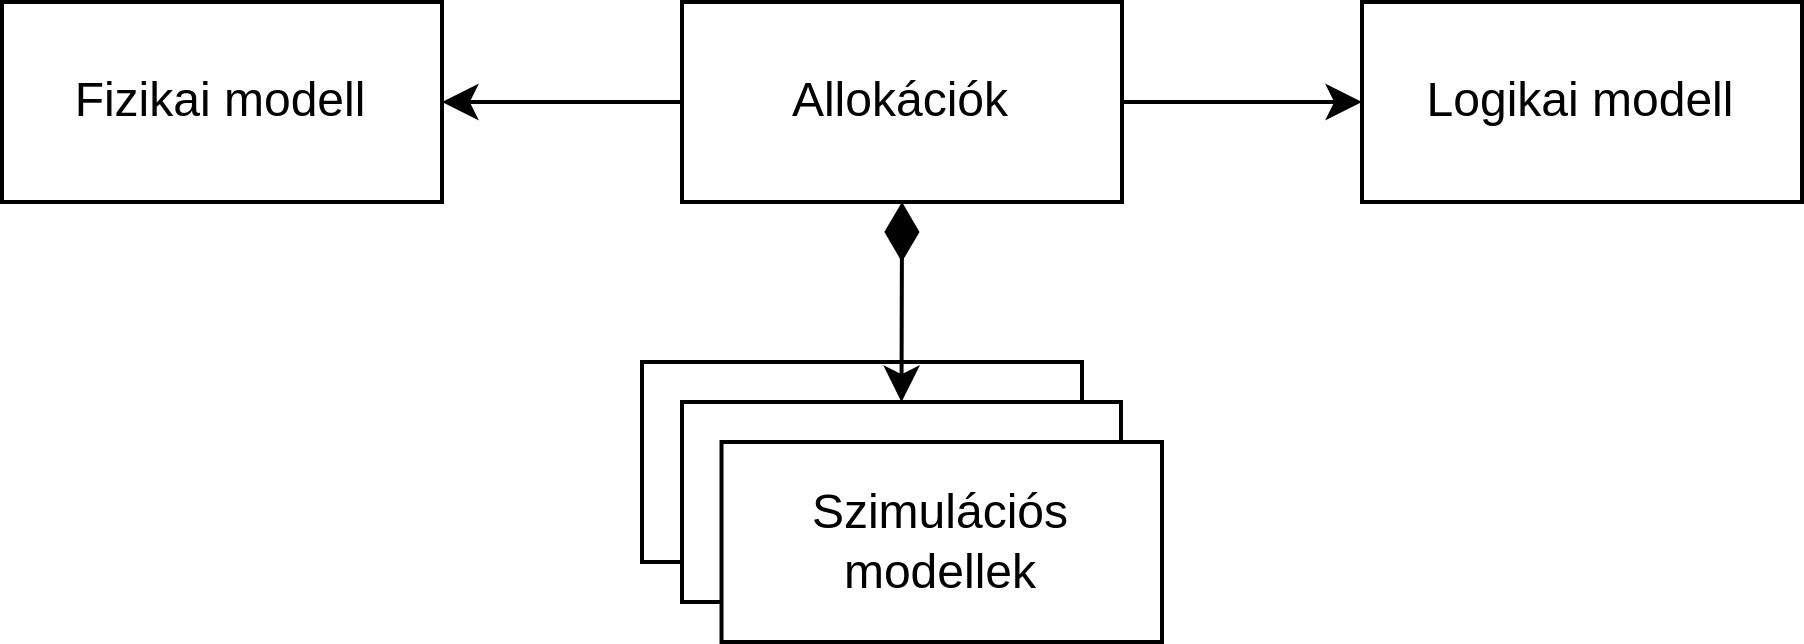
\includegraphics[width=150mm, keepaspectratio]{figures/Alapelemek.drawio.png}
            \caption{A modellek alapvető struktúrája} 
            \label{fig:Alapstruktura}
        \end{figure}

        Ennek oka, az a mögöttes gondolat, hogy a rendszereket igazából egy allokációval lehet leírni. Mivel ez a gondolat elsőre nehezen átlátható vegyünk egy példát.
        Amikor egy autót akarunk leírni, logikusnak tűnik egy \emph{Part} ként tekinteni rá --~ez a jelenleg bevett módszer is~--, mivel az \ref{sec:NyelviElemek} résznek megfelelően ez egy önmagában értelmes elem a modellben.
        Azonban amikor egy autóról beszélünk, akkor igazából valamilyen konkrét funkcióra és annak bizonyos megkötések mellett történő megvalósítására gondolunk.
        
        Nem nevezünk valamit autónak, csak mert úgy néz ki, mint egy autó, vagy ha más funkciót lát el. Ha egy óriáskerék kabinjait autókból építjük meg, akkor azokat a továbbiakban nem tekintjük autóknak, még akkor sem ha a folyamat során teljesen működőképesek maradnak, mert már nem az a funkció tartozik hozzájuk amit egy autótól elvárunk.
        Ugyancsak nem nevezzük autónak a Csillagok háborújának ikonikus homoksiklóját sem, hiába nyilvánvaló a nézőknek, hogy az autók megfelelői az adott világban. A szerkezete, amivel ezt megvalósítja eltér attól amit egy autótól elvárunk, mert forgó kerekek helyett lebeg és egy hajtómű tolja előre.

        Elsőre nehéz látni, miért fontos, hogy magát a rendszert egy másik absztrakt elemmel írjuk le, ha az eddigi megközelítés is működött. Ennek oka a későbbiekben fog látszani, mivel ez a személetváltás tette kiemelt elemmé az allokációkat a kidolgozott módszerekben.
        Tervezés közben magától értetődő gondolat, hogy a modellek finomítása attól függ milyen funkciót és milyen eszközzel akarunk megvalósítani.
        Ennek ellenére a bevett tervezői gyakorlatban az allokációkat inkább befejező lépésnek tekintik, nem a folyamat mozgatórugójának. Persze így is létrejönnek végül a modellek, de csak több iteráció után, amikor sikerült a logikai és fizikai nézeteket egymáshoz igazítani.
        A szemléletváltás után, amikor kiemelt figyelmet szentelünk ennek a megfeleltetési folyamatnak, felfedezhető, hogy ezek az információk, amelyek a fent leírt összeillesztést vezérlik, végig jelenvoltak az allokációkban, csupán figyelmen kívül maradtak a művelet helytelen szemlélete miatt.

        A szimulációs modellek is ezért kaptak helyet, az allokációkon belül, mivel azok a konkrét rendszert reprezentálják, ami a két modellnézet közti megfeleltetés.
        Ha másképpen hoznánk létre ezt a megfeleltetést a nézetek között vagy bármelyiket módosítanánk, akkor megváltoznának a szimulációs modellek is. Ebből látható, hogy ezek a modellek tényleg a rendszerhez, azaz az allokációkhoz tartoznak. Azzal, hogy az allokációk részei a szimulációs modellek egyértelművé válik melyik rendszerhez tartoznak, mert nem lehet őket elválasztani attól.

        \subsubsection{A modellek belső szerkezete} \label{sec:ModellekSzerkezete}
        Maga a módszertan javaslat három nagyobb fázisra osztható, melyek a \ref{fig:ModellStruktúra} ábrán láthatóak, különböző színekkel jelölve. Ezek egymás után, mindig az előzőre épülve jelennek meg, így a bemutatásuk is így történik a továbbiakban.
        Az ábrák konzisztensen ugyanazzal a színnel jelölik az adott fázishoz tartozó elemeket, megkönnyítendő az értelmezést.
        \begin{figure}[!ht]
            \centering
            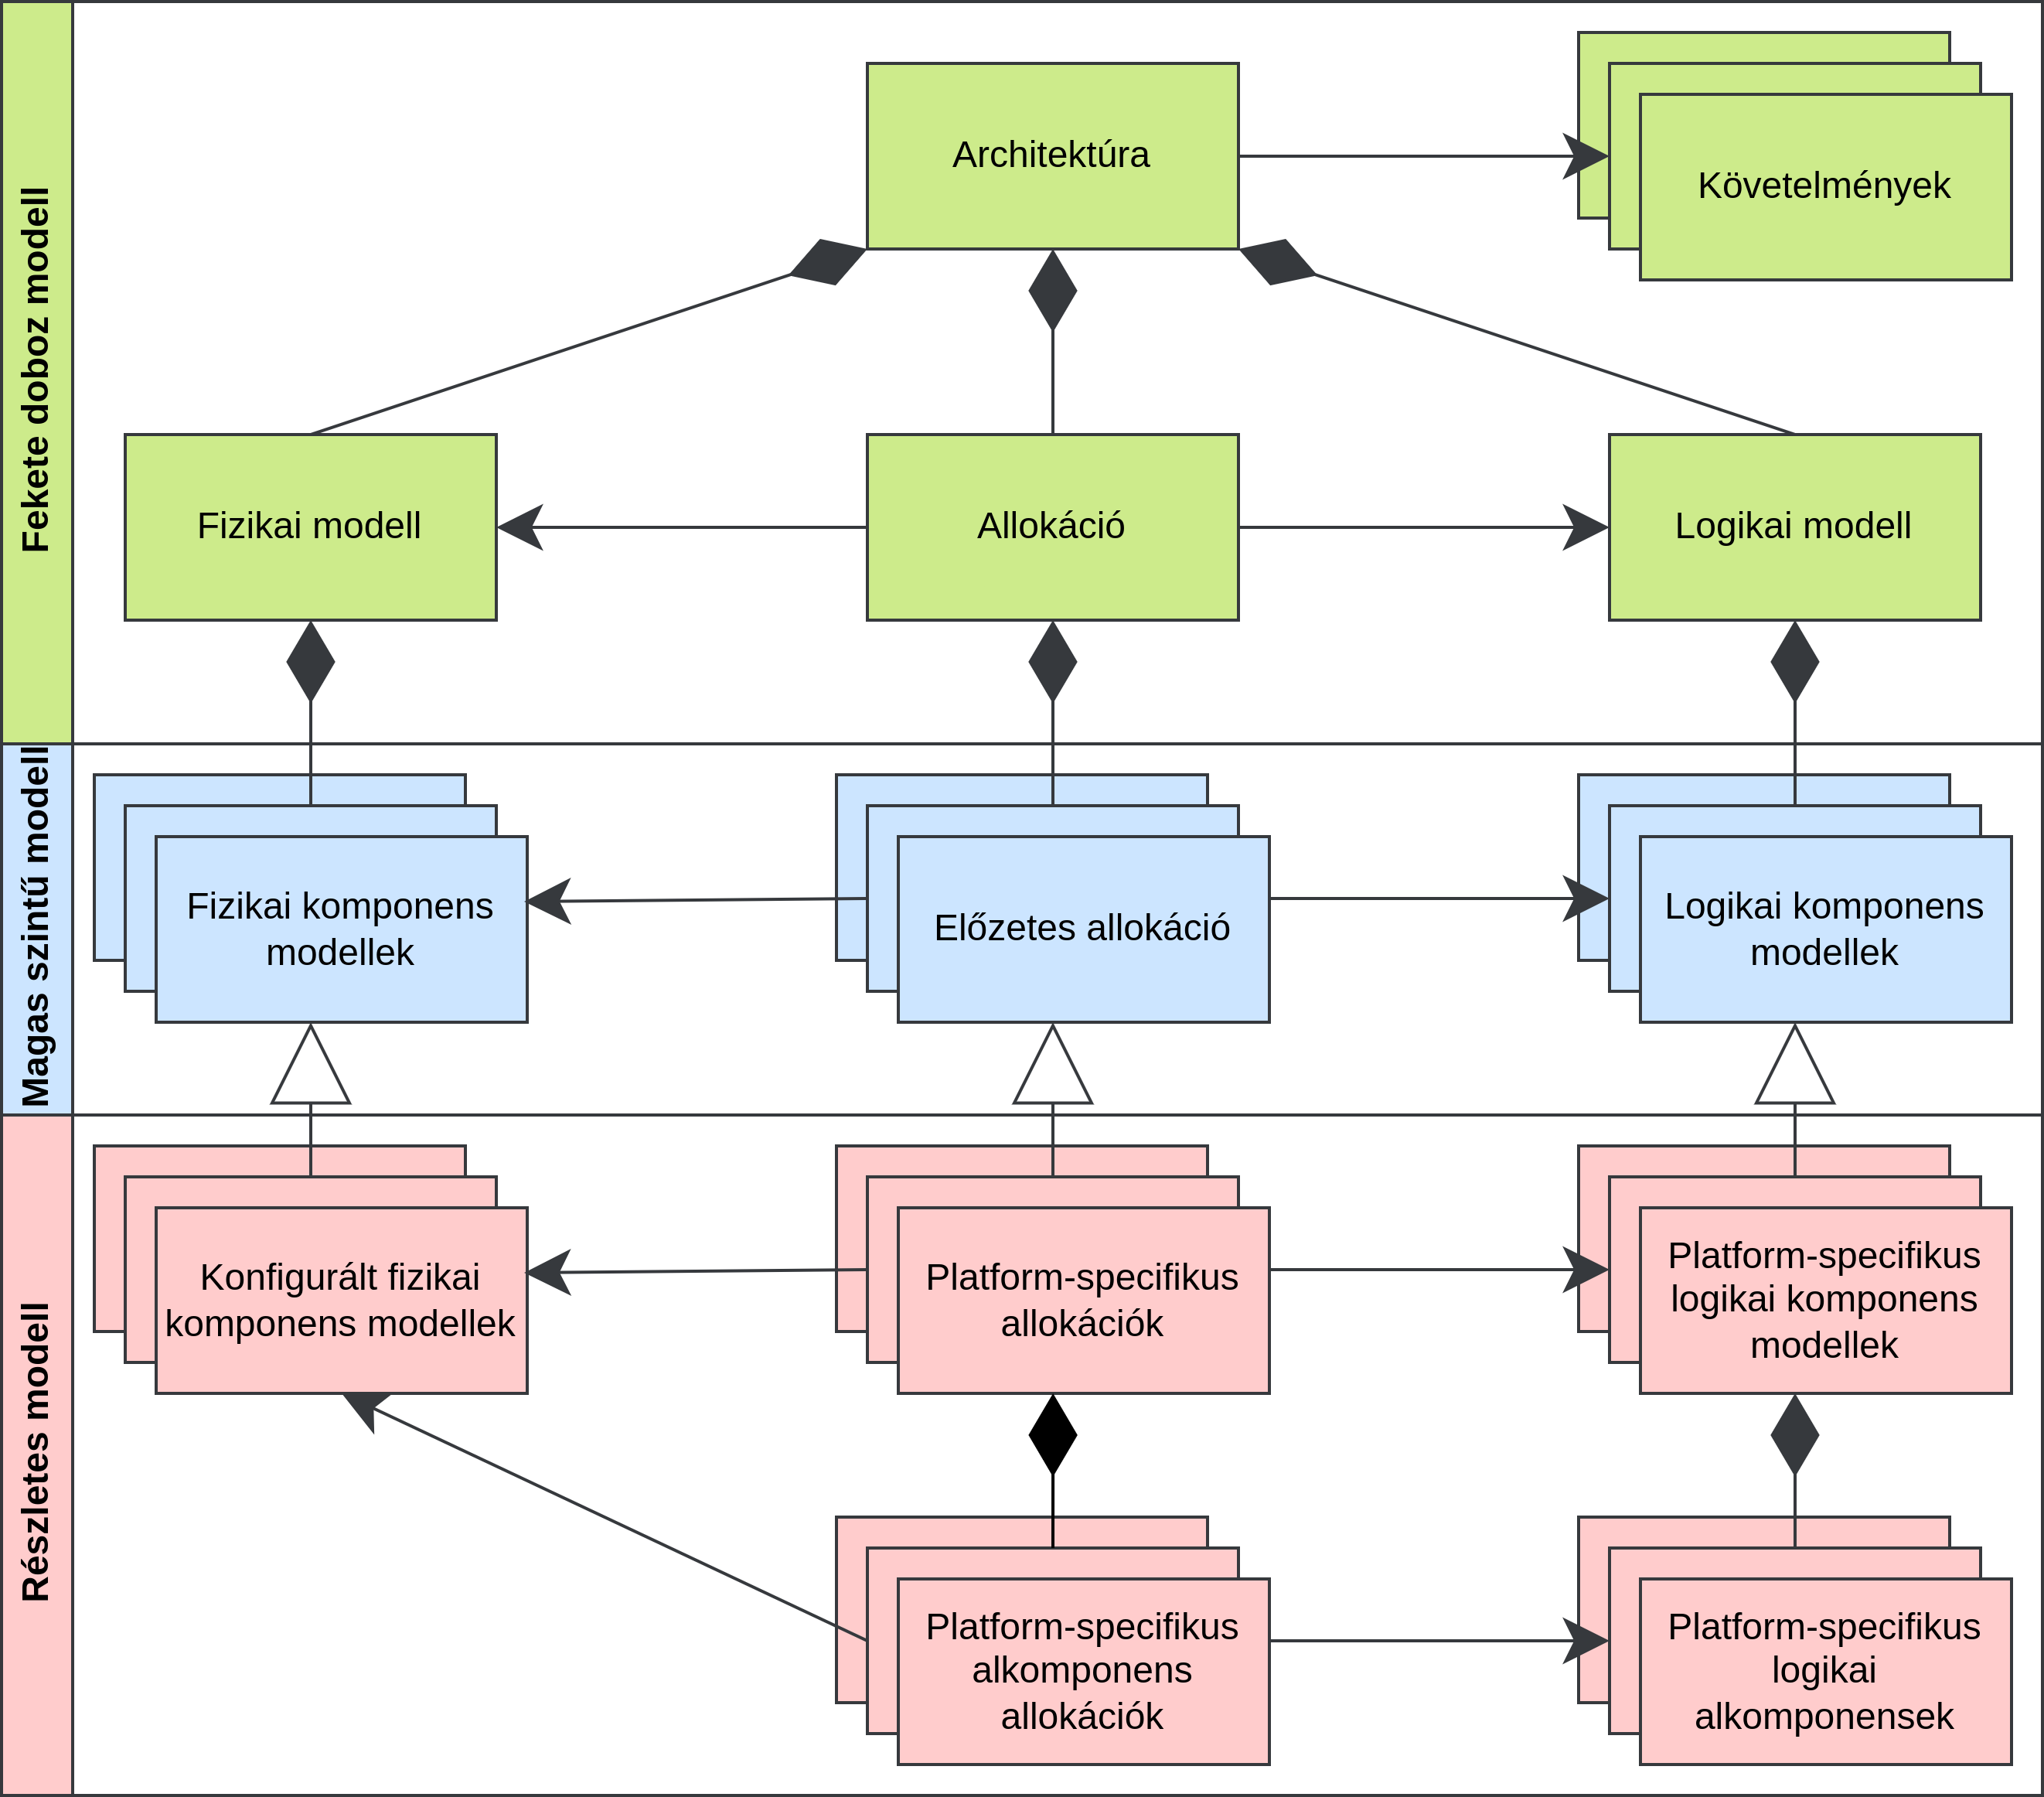
\includegraphics[width=150mm, keepaspectratio]{figures/AllocationBased2HU.drawio.png}
            \caption{A módszertan szerint készült modellek általános szerkezete} 
            \label{fig:ModellStruktúra}
        \end{figure}

        Az első fázis a \emph{Fekete doboz modell} összeállítása. Ebben a lépésben még semmilyen implementációval kapcsolatos kérdésről nem szabad dönteni, a hangsúly a rendszerrel szemben támasztott követelmények meghatározásán van.
        Az implementációs kérdések mellőzése azért kiemelten fontos, mert ha a tervezők elkezdenek egy konkrét megoldásban gondolkozni akkor az túl korán beszűkíti a lehetőségeket a megvalósítások tekintetében és elterelheti a figyelmet fontos kérdésekről a követelmények terén.
        A követelményeken kívül olyan előkészítő lépések kapnak még helyet ebben a fázisban mint a projektváz kialakítása, esetleg alkatrészkönyvtárak összegyűjtése, bár itt vigyázni kell nehogy implementációs kérdésekbe bonyolódjunk.
        A modell váza a \ref{fig:ModellStruktúra} ábrán látható a zöld színnel jelölt területen amely ennek a fázisnak felel meg.
        
        A \emph{Követelmények}-ben találhatóak a rendszerrel által teljesítendő követelmények és kapcsolódó használati esetek, míg a többi elem a projekt vázát adja meg. Ebben a vázban megfigyelhető egy gyökérelem, amely összefogja a rendszert, valamint látszik hogy ennek a rendszernek, mint egésznek kell teljesíteni a követelményeket.
        A rendszer váza tartalmazza továbbá a \ref{sec:Alapgondolatok} részben tárgyalt alapstruktúrát.
        Ezekben az elemekben találhatóak a rendszernek a környezete számára is ismert részei. Ezek az elemek a rendszer kontextusából, azaz beágyazó környezetéből ismertek.
        Például egy műhold esetében tudjuk, hogy milyen környezeti hatásoknak lesz kitéve a rendszer, milyen attribútumai vannak amelyek valamilyen érdekelt félnek fontosak, mint a tömeg és a méretek, illetve, hogy szükség lesz valamilyen vezeték nélküli kommunikációra amivel az eszköz kommunikálhat a földi irányítóközponttal. Utóbbinál fontos hangsúlyozni az implementációs kérdések mellőzését. Nem szabad belemenni olyan részletekbe, hogy rádiós, lézeres vagy valamilyen egyéb technológiát használunk majd, de az meg kell jelenjen, hogy lesz ilyen lehetőség, illetve a választandó technológia által teljesítendő követelményeket is össze kell gyűjtenünk. 
        Ezen túl ennek a váznak a szerepe, hogy a továbbiakban erre tudnak majd ráépülni a különböző modellrétegek.

        Ezután a \emph{Magas szintű modell} elkészítése következik. A logikai modellben definiáljuk, hogy milyen részfeladatokra bontva és hogyan oldjuk meg a rendszertől elvárt működés biztosítását.
        A fizikai modellben megadjuk milyen alrendszerek és alkatrészek segítségével biztosítjuk ezeknek a logikai feladatoknak az elvégzését.
        Végül az \emph{Előzetes allokációkkal} hozzárendeljük a feladatokat ezekhez a fizikai komponensekhez.
        
        A javasolt módszertan szempontjából legfontosabb részlet, hogy ezek az \emph{Előzetes allokációk} egyetlen logikai elemet több fizikaihoz is hozzárendelnek. Ez a végleges modellben már nem lenne előnyös, mert mindig pontosan egy felelősre van szükség egy adott feladat végrehajtásánál, de a magas szintű terveknél éppen ezt szeretnénk elérni.
        Ennek oka, hogy a fizikai és logikai nézeteket nem véletlenül választottuk külön, az egyes vetületekben a komponensek határai tipikusan eltérnek, átlapolódnak.
        Ha ez nem így lenne, akkor valószínűleg nem sikerült rendesen elválasztani a két nézetet, tehát ez egyik túl nagy mértékben meghatározta a másikat vagy már túlzottan belemerültünk az implementáció részleteibe. Mindkét eset könnyen vezethet szuboptimális megoldásokhoz és nehezen átlátható modellekhez. (Lásd: \ref{sec:LogFiz}. követelmény)
        
        A célunk, hogy ezeket a többszörös allokációkat és mögöttes jelentésüket fel tudjuk használni a modell további finomítása során. Ez a rejtett információ az, amely korábban sokszor iteratív finomítással került feltárásra, pedig helyes allokációkkal és azok vizsgálatával könnyen átlátható.
        A következő fázis előtt fontos kitérni arra, hogy mi is okozza pontosan a többszörös allokációkat, illetve milyen információt hordoznak a későbbi lépések számára.
        
        A fő ok, hogy a kérdéses logikai feladatot több fizikai komponens együttes munkája képes ellátni. Ebben az esetben ezt a feladatot tovább kell bontani az alapján, hogy milyen részfeladatokat melyik komponens valósít majd meg.
        Azért fontos, hogy ez a lebontás ne a magas szintű modellben történjen, mert annak feladata az adott probléma minél pontosabb megértése és hatékony megoldása, nem a konkrét implementáció elkészítése.
        Ha már ezen a szinten elvégeznénk a feladatok felosztását a fizikai komponensek függvényében, akkor az megnehezítené a modell átlátását, mert megfosztana minket a hierarchikus tervezési módszerektől amelyeket a \ref{sec:Hierarhia}. követelmény kifejtésében tárgyaltunk.
        
        A másik lehetséges ok a biztonságkritikus rendszerekkel szembeni követelményekből és azok teljesítéséből adódik. Név szerint a redundáns alrendszerekből. Ha csökkenteni akarjuk egy alrendszer meghibásodásának esélyeit akkor gyakran az egyetlen ésszerű megoldás az, ha több példányt is beépítünk belőle a rendszerbe, amelyek külön-külön is képesek ellátni a feladatukat.
        Ennek előnye, hogy annak jóval kisebb az esélye, hogy több is meghibásodik a kérdéses rendszerből\footnote{Ez az állítás csak független hibaokokat feltételezve érvényes. Ha ezt nem feltételezhetjük, akkor diverz tervezéssel védekezhetünk, ahol a duplikált alrendszerek nem pontos mások. Csak a velük szembeni követelmények azonosak, az implementáció minél eltérőbb, minimalizálandó az összefüggő hibaokokat. Például hiába használunk több GPS modult helymeghatározásra, ha nem az egyes modulok hanem maga a GPS hálózat válik működésképtelenné, akkor a redundancia önmagában nem nyújt védelmet.}, így tovább növelhettük a rendszer megbízhatóságát.
        A redundancia implementálása szintén későbbi lépésekben célszerű, felesleges bizonyos részfeladatok duplikálásával bonyolítani az áttekinthetőséget célzó magas szintű terveket, amikor ennek oka a konkrét implementációval szemben támasztott elvárások.

        A harmadik fázis a \emph{Részletes modell} megalkotása.Ebben a lépésben finomítjuk tovább a fentiekben leírtak szerint a modellt, hogy megkapjuk a már említett egy-egy kapcsolatokat létrehozó allokációkat.
        A \ref{fig:ModellStruktúra} ábrán látható, hogy ez esetben az új elemeket nem tartalmazza az eggyel korábbi lépés, hanem az új elemek \emph{specializálják} a magas szintű komponensmodelleket.
        
        Ennek oka, hogy a feladatoknak az egyes alkatrészek között több lehetséges felosztás is lehetséges. Azzal, hogy egy specializációval leválasztjuk ezt a réteget a magas szintű tervekről, lehetőségünk van több leszármazottat definiálni, amelyek a szimulációs modellek segítségével összehasonlíthatóak lesznek teljesítmény szempontjából.
        A több lebontás kapcsán gondolhatunk arra, hogy hogyan osztunk meg szoftverkomponenseket több processzor között a fogyasztás, válaszidő vagy pontosság alapján optimalizálva. De ugyanígy lehet szó arról, hogy a magas szintű modellben csak azt határoztuk meg, hogy egy adott gyártó melyik termékcsaládjából választunk például villanymotort egy adott feladatra, amely a vezérlés szempontjából már elegendő magas szinten, és csak a specializáció után választunk konkrét típust, amikor már pontosabb adataink vannak a várható terhelésről.

        Maga a lebontás először a logikai elemek dekompozícióját jelenti a fizikai komponensek alapján, ezzel létrehozva a \emph{Platform-specifikus logikai komponens modelleket}.
        A következő lépés a fizikai komponensek konfigurálása. Ez a különböző paramétereik meghatározását jelenti úgy, hogy ezzel készek legyenek a megfelelő feladatok ellátására.
        Ez lehet akár egy szabályozó paramétereinek hangolása, a memória kiosztása egy mikroprocesszoron, de konfigurálható logikai áramkörök esetében a konkrét áramkörök megtervezése és a megfelelő hardver erőforrások hozzárendelése is.
        Végül elkészítjük a \emph{Platform-specifikus allokációkat} is, amelyekben alacsonyabb szintű allokációkkal teremtjük meg a már említett egy-egy kapcsolatokat a \emph{Platform-specifikus logikai komponens modellek} és a \emph{Konfigurált fizikai komponens modellek} között.

        \subsubsection{A fejlesztés menete} \label{sec:flow}
        Az előző fejezetben már látható volt, hogy milyen főbb lépésekre tagolódig a rendszertervezés a javasolt módszerek használatával, de a modell szerkezete csupán egy egyszerűsített képet ad erről.
        Ebben a részben ez a folyamat kerül részletesebb bemutatásra.
        
        Maga a fejlesztési folyamat a \ref{fig:Folyamat} ábrán látható. Az ábra színezése megfelel a korábbiaknak elősegítendő a tájékozódást.

        Az első fontos észrevétel a szimulációs modellek újbóli megjelenése. Míg a \ref{fig:Alapstruktura} ábrán látható, hogy az allokációk szimulációs modelleket tartalmaz(hat)nak, míg a \ref{fig:ModellStruktúra} ábrán ezek nem voltak jelölve.
        Ez a változtatás csupán az ábra átláthatósága miatt történt, ezek a modellek továbbra is be vannak ágyazva az allokációkba, csupán az egyébként is összetett ábráról lettek lehagyva a megértés megkönnyítésének érdekében.

        \begin{figure}[!ht]
            \centering
            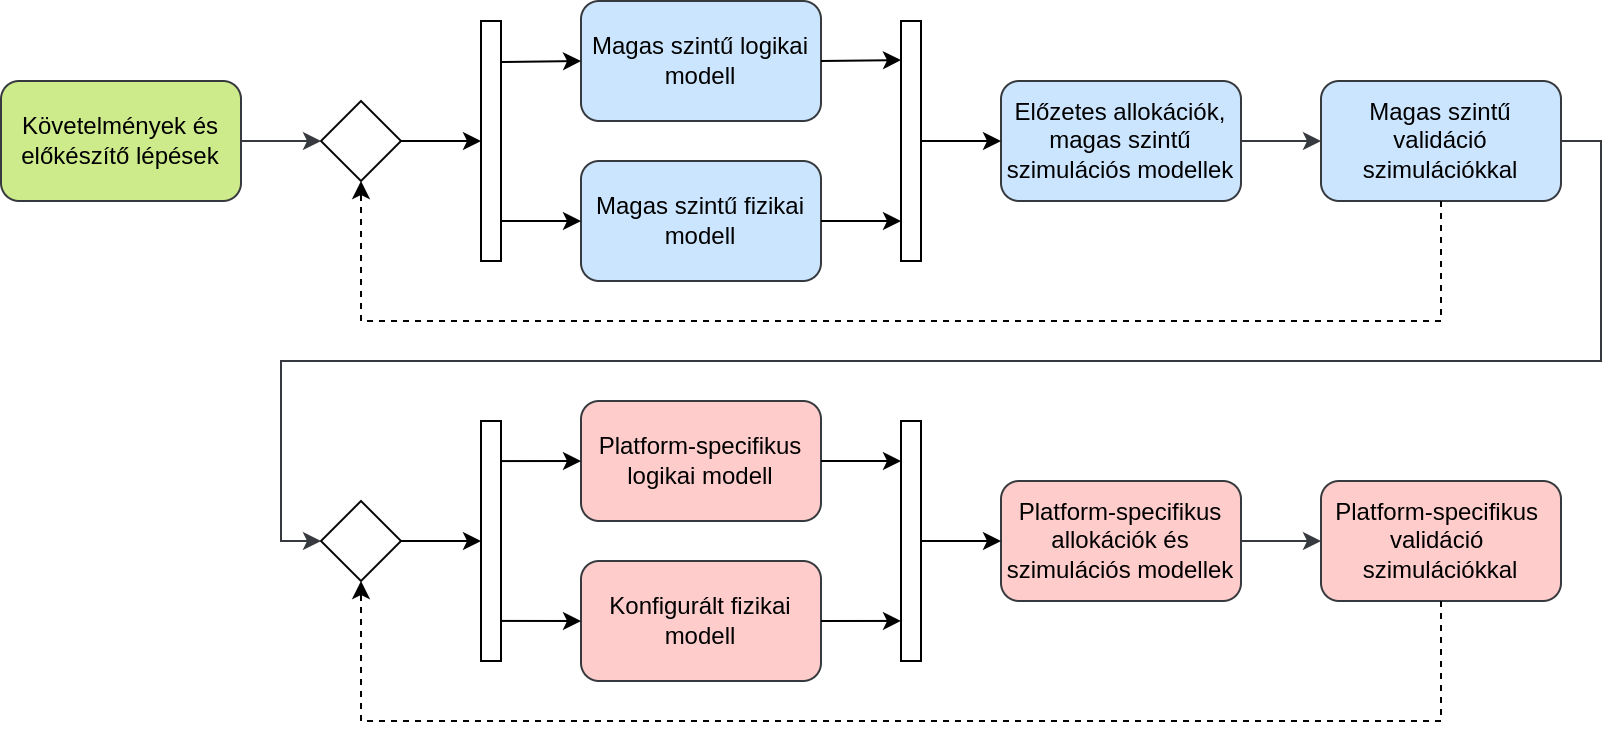
\includegraphics[width=150mm, keepaspectratio]{figures/ParalelAllocationBasedFlowHU.drawio.png}
            \caption{A fejlesztési folyamat menete} 
            \label{fig:Folyamat}
        \end{figure}

        Visszatérve a fejlesztés menetére, látható, hogy az első fázis a jelenlegi módszerek mellett egyetlen lépést igényel csak. A követelmények összegyűjtése és a javasolt módszertan által megkövetelt alapstruktúra létrehozása történik meg, a további munka előkészítéseként.
        
        A következő két fázis meglehetősen szimmetrikus, így azokat vizsgálhatjuk együtt. Először a logikai és fizikai modellek finomítása következik. Ez a két lépés haladhat párhuzamosan, mert az előző fázisokból szerzett információk alapján mindkét modell finomítása elkezdhető, de meg kell említeni, hogy a fizikai modell aktuális bővítésének befejezéséhez gyakran szükséges a logikai modell elkészítése. Erre jó példa a \emph{Konfigurált fizikai komponensek} esetén egy mikrovezérlő memóriatartományának felosztása.
        Ugyanakkor a redundáns alrendszerek duplikálása nem igényli a pontos logikai modellt, így azt célszerű azzal párhuzamosan végezni.
        
        A folyamatábráknál az ilyen párhuzamosság jelölés azt jelenti, hogy a feladatok végrehajtásának sorrendje nem ismert, tehát nemcsak valódi párhuzamosságot jelöl a fenti ábra, csak pontos sorrend nélkül végezhető feladatokat.
        A kidolgozott módszertan javaslatban ez a sorrend az alkalmazott tervezési irányelvektől függ. Így megengedett top-down, bottom-up és kevert módszerek alkalmazása is. Fontos megemlíteni még az autóiparban egyre inkább elterjedő platformalapú módszereket, ahol a fizikai modell megelőzi a logikait, mert annak alapja többnyire már adott a rendszer tervezése előtt, lényegi változtatás csak az utolsó, konfigurációs fázisban történik rajta.
        Egy fázisokra bontott, és adott lépésben megengedőbb módszertan éppen azért célravezető, mert a lehető legkevésbé köti meg a módszer alkalmazóinak kezét az alkalmazandó tervezési irány tekintetében, elősegítve a széleskörű alkalmazhatóságát.
        
        Ha elkészült a két modellnézet, akkor létrehozhatjuk az adott szinthez tartozó allokációkat és ezek alapján elkészítjük az új, részletesebb szimulációs modelleket.
        Végül mindkét fázisban felhasználjuk a szimulációs modelleket, hogy validálhassuk az új modelleket mielőtt továbblépnénk a következő fázisra. Természetesen nem csak szimulációt használunk validációra, de a javaslatok újdonsága ezeknek a technológiáknak a támogatása.
        
        Amennyiben a validáció nem sikeres egy új iterációban megismételjük az adott fázist. Fontos, hogy ez az iteráció a validáció elbukásának következménye, a korábbi módszerekben megjelenő iteratív illesztést a logikai és fizikai modellek között már feloldottuk, ezt a típust pedig nem lehet.
        Ha sikeres volt a fázis végén a validáció, akkor tovább lépünk a módszertanban.
        
        Ezeknél a validációs méréseknél van lehetőség végrehajtani a \ref{sec:ModellekSzerkezete} részben említett kiértékelést a különböző implementációk között, mivel itt egyébként is futtatunk ilyen méréseket a továbblépés előtt.
        Ezen túl meg kell említeni, hogy a javasolt módszerek alkalmazhatóak az egyes alrendszerek kapcsán is. Az első fázis itt az adott alrendszerre vonatkozó követelmények összegyűjtése, ezután pedig a módszertan lépései ugyanúgy ismételhetők az adott komponensen belül.
        Szintén alkalmazható ez a módszer a rendszer kontextusának modellezése során, ilyenkor gyakorlatilag egy olyan modellt alkotunk meg, amelynek a rendszerünk csak egyetlen eleme, célja pedig a környezeti elemek egymással és a rendszerrel való kölcsönhatásainak leírása.
        Ilyen modelleket minden módszertan használ a fejlesztés elején (Lásd: \ref{sec:KorabbiModszerek} rész), sajnos ennek a lépésnek a részletes vizsgálatára a dolgozat kereteiben nem volt lehetőség.

        \subsubsection{A könyvtárak szerkezete és használata}
        Ahogy az a \ref{sec:Ujrahasznalas}. követelménynél is olvasható volt, a tervezés során gyakran felmerül az igény az egyes komponensek újrahasználására, esetleg külső beszállítótól való beszerzésére.
        Ennek megkönnyítésének érdekében a módszertannak támogatni kell komponenskönyvtárak létrehozását és használatát is.
        A módszertanhoz kidolgozott könyvtárstruktúra a \ref{fig:Konyvtar} ábrán látható.
        \begin{figure}[!ht]
            \centering
            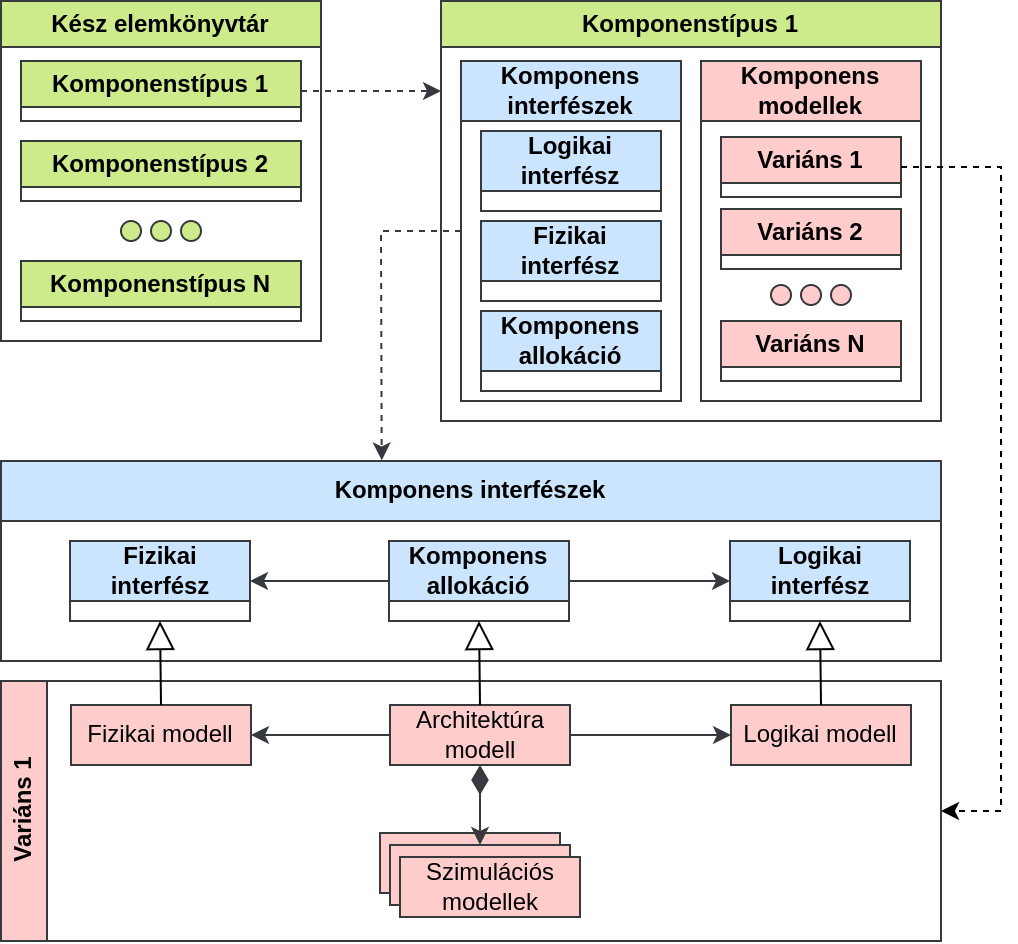
\includegraphics[width=150mm, keepaspectratio]{figures/InterfaceParts.drawio.png}
            \caption{A komponenskönyvtárak szerkezete.} 
            \label{fig:Konyvtar}
        \end{figure}

        A könyvtáron belül komponenstípusok vannak. Ezekbe a kifelé --~a paramétereiket leszámítva~-- azonosan megjelenő komponensek kerülnek csoportosításra, mint például szervomotorok, egyenáramú motorok, stb.
        Egy komponenstípuson belül definiálva van egy általános komponens-interfész, amely egy alapvető modell, amely a külvilág által látható elemeket tartalmazza a komponenstípusra vonatkozóan. Ez az alapvető fizikai és logikai modellből valamint az azokat összekötő allokációs típusból áll.
        
        Az allokációhoz azért célszerű külön típust bevezetni, mert megadható benne, hogy milyen típusú elemeket képes allokálni, így csökkentve a hibalehetőségeket.
        
        Ezenkívül minden konkrét komponenshez tartozik egy-egy ilyen komponens-specifikus típus is, amely \emph{specializálja} az általános verziót.
        
        Ennek azon túl, hogy illeszkedik a kidolgozott módszertanba két előnye van.
        Először is a specializált allokációban szűkíthetjük a végekre vonatkozó típuskövetelményeket, hogy csak az összetartozóakat fogadja el a konkrét komponensmodellekből, ezzel is csökkentve a modellezési hibák előfordulását.
        Másodszor pedig, az azonos típusú komponenseknek a legtöbb esetben csak apróbb eltérések jelentkeznek a szimulációs modelljeiben, a legjellemzőbb, hogy csak paramétereikben térnek el.
        
        Ha a megfelelő szimulációs modellvázak szerepelnek az általános allokációban, akkor a konkrét típusnál elég a paramétereket felülírni és azt a néhány kisebb módosítást redefiniálni, ha ez szükséges.
        
        Ezzel csökkenthető a kódduplikáció, megkönnyítve a könyvtárak karbantartását. Ez azért is fontos, mert a \ref{sec:fmi}-ben megismert FMI szabvány által definiált csomagok, amelyeket a gyártók biztosítani szoktak a megrendelőiknek szimulációs célra szintén paraméterezhetőek, illetve relative nagy méretűek a rendszermodellekhez képest.
        Ha tehát ezekből minél kevesebbet kell a könyvtárral együtt tárolni, akkor azok mérete radikálisan csökkenthető.

        \subsubsection{Szimulációs modellek használata}
        Mivel a módszerek kidolgozásánál külön cél volt a szimulációs technológiák integrálása, ezért tekintsük át az ezekre vonatkozó részeket.
        
        A szimulációs modellek rendszermodellen belüli reprezentációival kapcsolatos elvárások a \ref{sec:SzimIntKov}. követelménynél olvashatóak. A legfontosabb követelmény, hogy több szimulációs modellt is támogasson a módszertan egy adott komponenshez, teljesül, mivel több is hozzárendelhető az allokációkhoz.
        Ezeknek a modelleknek a finomítása ráadásul folyamatosan történik a módszertan folyamán, a rendszerrel együtt fejlődnek és szerves részét képzik a fejlesztési folyamatnak, a tervezői döntéshozásnak.
        
        Ezzel elérhető a \ref{sec:mbseElonyei} és \ref{sec:szimElonyok} részekben leírt minden fejlesztési fázisban jelenlévő V\&V tevékenység és gazdaságosság, mivel a módszer a lehető legkorábbi fázisban kiszűri a koncepcionális vagy implementációs hibákat.

        Azzal, hogy a nagyobb fázisokban hierarchikusan helyezkednek el az egyes allokációk, támogatható, hogy egy magasabb szinten lévő modell hivatkozzon az általa tartalmazottakra, így a szimulációs modellekre is kiterjesztődnek a \ref{sec:Hierarhia}. követelménynél tárgyalt hierarchikus módszerekre vonatkozó előnyök.
        
        Mivel a hierarchiában minden szint több szimulációs modellt támogat, így hierarchikus szimulációs modellek használatával még egyszerűbbé válik a különböző részletességű szimulációs modellek készítése, mivel a az alkomponensek esetén elég a használt szimulációs modellek hivatkozásait redefiniálni.

        \subsubsection{Kontextus modellezés}
        A rendszertervezési módszertanokban (Lásd: \ref{sec:KorabbiModszerek} rész) rendszerint a rendszer modellezése mellett nagy hangsúlyt helyeznek annak kontextusának, azaz beágyazó környezetének a modellezésére. Fontos tehát ezt a területet is részletesen megvizsgálni, hogy minél közelebb kerülhessünk egy teljes, gyakorlatban is jól alkalmazható módszertanhoz.

        A rendszer kontextusa az, ami meghatároz számos követelményt, illetve azt, hogy a rendszer hogyan lép interakcióba a környezetét alkotó elemekkel.
        Ezek azok a kapcsolódási pontok és követelmények, amelyek a már bemutatott módszerekben a fejlesztés első fázisában jelentek meg, tehát nem meglepő, hogy ez az alfejezet ahhoz a lépéshez tartalmaz kiegészítéseket.
        
            \paragraph{A nézetek fontossága}
            Elsőre kérdéses lehet, hogy a kontextusmodellnél is szükséges-e a logikai és fizikai nézetek elválasztása.
            A válasz igen, de a megértéséhez célszerű egy konkrét példát venni.
            
            Ha egy műholdat tervezünk, akkor szeretnénk vele kommunikálni a földről. Ez történhet egyetlen földi állomásról is, de van, hogy jóval többet akarunk kommunikálni, mint amennyit egyetlen földiállomás lehetővé tenne. Ilyenkor erre a célra használhatunk több földiállomást is, amelyek azonban lehet hogy nem egyformák. Ilyenkor a fizikai modellben lehet hogy teljesen más frekvenciasávon, sávszélességen és modulációval valósul meg a kapcsolat, de logikailag nincs feltétlenül különbség.
            Ilyenkor azt szeretnénk, hogy a logikai modell a lehető legegyszerűbb maradjon, de a fizikaiban megjelenjenek ezek a részletek is, mivel ezek fontosak a fejlesztés szempontjából.

            A szétválasztás azért is fontos, mert a rendszer esetében is jellemzően más-más szakemberek dolgoznak ezeken a területeken. Ez valószínűleg a kontextusmodell esetében is így van, de ha mégsem, akkor is célszerű úgy elkészíteni ezt a modellt, hogy az könnyen használható legyen a továbbiakban.

            \paragraph{Analógiák az egyes fázisok során}
            Azért fontos külön foglalkozni a kontextusmodellel, mert jellemzően nem pontosan ugyanaz a folyamat szükséges az elkészítéséhez, mint a rendszermodell esetében, de a főbb gondolatok továbbra is azonosak.
            Vegyük végig a korábban bemutatott fázisokat a kontextusmodellre nézve és vizsgáljuk meg, hogyan alkalmazhatóak ehhez a modelltípushoz.

            A kontextus \emph{Fekete doboz modelljének} elkészítése során a már ismert követelményeket ugyanúgy felvesszük, azonban a logikai és fizikai modellek esetében nem jelennek meg a rendszernél látott külvilág számára ismert elemek.
            Ennek oka, hogy a kontextus maga is egy rendszer, méghozzá zárt. Nincsenek tehát, olyan kívülről ismert elemei mint magának a megtervezendő rendszernek. Ha lennének ilyen elemei, akkor azok a kontextus kontextusához kapcsolódnának és ez a folyamat talán sosem érne véget.
            Az, hogy hol állunk meg, mi tartozik a kellően részletes kontextusmodellhez és mi az ami már felesleges részlet, természetesen már egy tervezői döntés. A javasolt módszerek nem adják meg hol húzzuk meg ezt a határt, csupán a létét követelik meg, hogy a valódi rendszerek modellje is kezelhető mértékű maradjon, ezzel a zárt világ szemlélettel.

            A rendszerünk célja, hogy valamilyen formában interakcióba lépjen a környezetével. A kontextusmodell megadja, hogy milyen feltételezésekkel élhetünk majd a tervezés során, illetve milyen követelményeknek kell megfelelnie a rendszernek, hogy megfelelő módon interakcióba a környezetével.
            Megfordítva, a rendszerünkre vonatkozó követelmények azok a feltételezések, amelyekkel a beágyazókörnyezet él a rendszerünk kapcsán. Mivel a környezetünk feltételezéseit rendszerint nem tudjuk megváltoztatni, így számunkra követelmény, hogy megfeleljünk ezeknek a siker elérése érdekében.

            A \emph{Magas szintű modell} szintjén kezdjük el kibontani a kontextusmodellt. Ebben az esetben nem funkciók és alkatrészek jelennek meg, hanem a rendszer és kontextusának elemei, valamint az egyes elemek közti kapcsolatok.
            A cél a kontextust addig finomítani ebben a lépésben, hogy minden fontos szereplő megjelenjen.
            
            A korábbi műholdas példában a rádiós kapcsolatok esetén például foglalkoznunk kell a különböző zajokkal.
            Ezek a logikai modellben elég ha zajként megjelennek, mivel a szerepük itt az, hogy a feladatoknál később foglalkozzunk a zajszűréssel.
            Ellenben a fizikai modellnél szeretnénk lebontani ezt szűkebb csoportokra. Például származhat a zaj más kommunikációs eszközökből, lehet háttérsugárzás, de akár aktívabb naptevékenység is. Ezek tipikusan másképpen viselkednek és másképpen is lehet védekezni ellenük a fejlesztés során, hiába ugyanaz a feladat logikailag.

            A \emph{Részletes modellben} a konkrét implementációhoz kapcsolódó elemekkel bővítjük az eddigi modellt. Ide tartoznak például, hogy egy rádiós kapcsolat milyen paraméterekkel valósul meg a rendszer és kontextusa között.
            Milyen frekvenciasávot és modulációt használunk, milyen protokollt kell betartanunk. Ez az a szint, amely hasonló rendszerek esetén is eltérhet, például két különböző műholddal szemben hasonlóak a magasszintű elvárások, azonban a konkrét feladatuk már számos különbséget határoz meg, amelyek eltérő kontextusmodellt eredményeznek.
            Azzal, hogy a kontextusmodellben is elválasztjuk a ezeket a szinteket, elősegítjük, hogy ezek a modellek is részben újrahasználhatóak legyenek.

            Feltéve, hogy a műholdas példát egy műholdgyártó cég szemszögéből nézzük, szeretnénk, ha lenne egy stabil alapunk a termékeink tervezésénél. Az első két fázis nagyrészt megegyezik az egyes megrendelések között, ha egyszer jól elkészítjük ezeket a modelleket, akkor az újrahasználásuk nem csak gyorsabbá, de biztonságosabbá teszi a tervezési folyamatot, mert a jövőben nem maradhatnak ki a már ismert tényezők a modellből.
            Az egyes megrendelésekben csak a \emph{Részletes modellt} kell mindig újra elkészíteni a konkrét igények kapcsán, de ez már ráépül a meglévő, biztos alapokra.
            
            Ez a megoldás hasonló az autóiparban jellemző platformalapú módszerekhez, mert csak a pontos feladathoz kell igazítani a meglévő eszközöket, bár ebben az esetben inkább egy keretrendszerről beszélhetünk az adott feladat kapcsán.
            
            \paragraph{Az allokációk fontossága}
            A rendszertervezés során kiemelt figyelmet kaptak az allokációk. A kontextusnál ez a szerep továbbra is megmarad, mivel a nézeteket továbbra is össze kell kötni és a szimulációs modelleknek is meg kell jelenni a modellben.

            Továbbá láttuk, hogy továbbra is jelen van egy folyamatos finomítás a módszerekben kibontandó hierarchiákkal, amelyek kezelésére szolgál az általam bevezetett allokációkon alapú modellezési szemléletet.

            Az allokációk szerepe azért is fontos továbbá a kontextusmodellben, mert azt szeretnénk, hogy a rendszermodell pontosan illeszkedjen a kontextusmodellbe, amihez elengedhetetlen az azonos struktúra.

            \paragraph{A rendszer megjelenése}
            Felmerülhet az a kérdés, hogy hogyan jelenik meg maga a rendszer, amelyre több válasz is adható.
            A kérdés onnan ered, hogy a rendszerünk nem feltétlenül egyetlen elem, hanem több különálló egység, azaz rendszerek rendszere.
            Ez kiemelten fontos elosztott kiberfizikai rendszerek esetén, ahol egy-egy eszköz tipikusan limitált képességekkel bír és több egység együttműködésével oldható meg egy feladat.
            Ilyenkor a rendszer elemei egyben egymás kontextusát is alkotják.

            Ha tényleg egyetlen elemünk van, akkor természetesen ez egy egyszerű kérdés, a rendszert egy elem reprezentálja.
            Jó megközelítés lehet ez akkor is, ha egy adott csapat készíti el az összes komponenst, mert így először a teljes rendszerre összpontosíthatnak és az így feltárt követelményeket később felhasználhatják a rendszer komponenseinek lebontásánál.
            Ez a megközelítés akkor is jól működik, ha előre nem tudjuk, hogy szükség van ilyen lebontásra, vagy nem ismert pontosan, milyen lebontásra lesz szükség.

            Ha viszont előre ismerjük a lebontást, vagy a komponenseket több külön csapat fejleszti majd, akkor felvehetjük előre az egyes komponenseket is az előbb bemutatott hierarchia alkalmazása nélkül is. Így minden alrendszernek elkészítve a kontextusmodelljét.

            A két módszer között nincs egyértelmű sorrend, az alkalmazásuk inkább az adott projekttől és a fejlesztő szervezet struktúrájától, esetleg saját konvencióktól függ, az is elképzelhető, hogy ezeknek egy kombinációját használjuk és még több hierarchiát vezetünk be.
            Ez csupán egy kitekintés, amely modellezési javaslatokat vezet be a módszerek esetleges alkalmazóinak.

            \paragraph{A rendszer fejlesztése a kontextusmodell alapján}
            A kontextusmodellt elsősorban a rendszerek fejlesztésének elősegítéséhez alkotjuk meg a kezdeti lépések között, de látható, hogy a rendszer tervezésének első lépéseivel együtt jön létre.

            Azzal, hogy a fentiek szerint a rendszermodellel összhangban álló struktúrát alkalmaztunk ehhez a modellhez is, lehetőségünk nyílik arra, hogy a kettőt szorosabban összefűzzük, hiszen két azonos modell elkészítése a rendszerről felesleges lenne, csupán hibalehetőségeket vinne a tervezési folyamatba.

            Ehelyett megtehetjük, hogy a rendszernek egyetlen modellje van, amely be van ágyazva a kontextusmodellbe. Ez a továbbvitele annak a korábbi gondolatnak, hogy a kontextusunk egy ugyanolyan rendszer, mint a miénk, csupán egy zárt világban. Ennek a világnak az egyetlen része, amit tetszőlegesen alakíthatunk, az a saját, általunk tervezett rendszer, ami így folyamatosan kerül kibontásra, a kontextusmodellel együtt.

            A módszer előnye, hogy nincs két független modell a rendszerünkről, szóval ezek nem is kerülhetnek inkonzisztens állapotba, a nyomonkövethetőség sokkal egyszerűbben garantálható, mit két külön modell esetén.

            \paragraph{A szimulációk szerepe}
            A szimulációk szempontjából a kontextusmodellnek kiemelt szerepe van. Mivel a javasolt módszerek szempontjából kiemelten fontosak a szimulációk, így célszerű ezt a szempontot is megvizsgálni a kontextusmodellek kapcsán.

            A szimulációk lényege, hogy a rendszerünk egy virtuális megfelelőjét egy virtuális környezetben tudjuk vizsgálni, ezzel elkerülve, vagy legalább csökkentve a fizikai teszteléssel járó időszükséglet és költségek mértékét.

            A kontextusmodell az, amely a teljes rendszerre nézve leírja ezt a virtuális környezetet, tehát ha nem csak egy-egy komponenst akarunk így validálni, akkor elengedhetetlen egy ehhez megfelelő kontextusmodell elkészítése.

            Bár a rendszer tervezésénél a \emph{Fekete doboz modell} elkészítésénél még nem alkalmaztunk szimulációkat, a kontextusmodellezés esetén mégis hasznos lehet.
            
            Vegyük a korábbi műholdas példát. A különböző rádiós berendezések költségesek így szeretnénk minél kevesebb ilyen alrendszert felhasználni a műholdunkhoz, de legalább annyi kell, hogy megbízhatóan kommunikálhassunk a műholddal a szükséges gyakorisággal.
            A különböző kommunikációs-alrendszer konfigurációkat szimulálva meghatározhatjuk azok hatékonyságát különböző szituációkban, ahol esetleg különböző meghibásodások és zavarok is könnyen figyelembe vehetőek.
            Egy ilyen vizsgálat csupán a műhold pályájának és a földiállomások felszerelésének, helyzetének ismeretét igénylik, amelyek megjelennek a kontextusmodellben, így a követelményeknél megadható, milyen paraméterekkel kell tudjon a rendszerünk kommunikálni.


\chapter{Eredmények értékelése}
A kidolgozott javaslatok esettanulmány alapján történő, illetve általános értékelése jelen fejezetben találhatóak.

\section{Kvadkopter esettanulmány}
A fent leírt módszerek tesztelése és továbbfejlesztése érdekében, szükség volt egy esettanulmányra, amelyen valóshoz hasonló körülmények közt is ki lehet próbálni az elméleti eredményeket.
Erre a célra egy olyan példa rendszerre van szükség, amely kellően bonyolult az előnyök kimutatására, az esetleges hiányosságok feltárására, de kezelhető méretű és lehetőleg széles körben érthető, hogy később demonstrációs eszközként szolgálhasson.

Ezek alapján a követelmények alapján egy kvadkopterre esett a választás. Pontosabban egy olyan négyrotoros drónra, amelynek az esettanulmányban a feladata, hogy szeles környezetben egy előre meghatározott pozícióban lebegjen.

Mivel az automatikus kódgenerálásra és a modellek konzisztenciájának ellenőrzésére még nincsenek eszközök, ezért ezeket a lépéseket manuálisan kellett elvégezni.
A következőkben először a rendszermodell, majd a szimulációs modell kerül bemutatásra, az elkészítésük során gyűjtött tapasztalatokkal együtt.

    \subsection{A rendszermodell}
    A rendszermodell esetében csak a főbb tervezési szempontok és a felépítés kerül bemutatásra, mert a dolgozat lényegének megértésében a konkrét forráskód elemzése nem segíti az olvasót. Ehelyett a struktúra bemutatása és a módszertan szempontjából lényeges részletek kiemelésére helyezem inkább a hangsúlyt ebben a részben.
    
    Az esettanulmány keretében a rendszer egy előre meghatározott pozíciót próbál tartani, így a kontextusmodellben csupán a szél jelenik meg külső befolyásoló elemként.
    A szelet a drón tömegközéppontjában ható erőként és forgatónyomatékként modelleztem, ezek mértéke az idő függvényében, a szimulációs modellben paraméterként adható meg, elősegítve a különböző terhelések vizsgálatát.

    A modellezett kvadkopter fizikailag igen egyszerű felépítést követ. Egy GPS és egy IMU modul segítségével méri a pozícióját és az orientációját. A példa egyszerűsége miatt ezek ideális szenzorként lettek modellezve.
    A módszertanban leírtak szerint ezt a modellt egy újabb iterációban lehetne tovább finomítani, de jelenleg tökéletesen megfelelő ez az absztrakció.
    
    A szenzorok adatait egy mikrokontroller olvassa, amely futtatja a szabályozó algoritmusokat, majd az azok eredményeképpen adódó motorvezérlő jeleket továbbküldi a négy motornak.
    
    A tervezés folyamán a motorokat kész komponensnek tekintettem amelyek a hozzájuk tartozó vezérlővel és rotorral egybeépítve készen kaphatóak. Ezek az egységek ipari drónok esetében valóban így kaphatóak katalógus szerint és saját adatlappal rendelkeznek, mert ezek a komponensek együtt határozzák meg a meghajtás különböző karakterisztikáit.
    Ezt azért fontos kiemelni, mert ez egy remek lehetőség kipróbálni a módszertanban javasolt könyvtárak használatát, illetve később a szimulációs modellben az FMU-k bemutatására is remek lehetőséget nyújt.
    
    A logikai modellben a szenzorok adatainak begyűjtése, a szabályozóalgoritmus és az az alapján történő beavatkozás jelenik meg magas szinten.
    
    Utóbbi kettő azért érdekes, mert így a magasszintű modellben nem köteleződtünk el egy konkrét implementáció mellett, mivel számos megvalósítás lehetséges egy forgószárnyas drón megvalósítására. Ennek az előnye többek között, hogy a pozíciótartásért felelős szabályozó csak az összesített tolóerőt és a különböző forgástengelyek mentén jelentkező elmozdulást állítja így ez gyakorlatilag teljesen független a rotorok számától és elhelyezkedésétől.
    Ez persze azt jelenti, hogy a szabályozó kimenetét nem lehet azonnal a motoroknak küldeni, hanem előbb elő kell állítani belőlük a konkrét beavatkozószervek utasításait.
    
    Ezzel a megoldással a szabályozónk újrahasználható elemmé vált, amelyet csak paraméterezni kell egy új hasonló rendszer esetében, ami egy valós projektnél előnyös gyakorlatnak számítana.
    
    Ezek alapján a beavatkozó blokk a későbbiekben tovább lett finomítva, hogy az általános parancsok alapján meghatározza az egyes motorok tolóerejét az adott konfigurációhoz. 
    Ezzel együtt finomításra került a két adatgyűjtési feladat a konkrét mérésre, valamint annak a szenzorból való kiolvasására és feldolgozására.
    
    Ennél a két esetnél jól megfigyelhető hogy a logikai és fizikai elemek átlapolódnak. Az adatgyűjtés két fizikai elemet is érintett, a beavatkozás pedig ötöt is, a transzformáció és a négy motor vezérlése által.
    
    Ezek az átlapolódások jól láthatóak voltak a magasszintű allokációk elkészítésénél, a következő fázisban a felhasználásikkal egyszerűen, egy lépésben elvégezhető volt a modellek finomítása az iteratív próbálkozás elkerülésével.


    \subsection{A szimulációs modell}
    A rendszer fejlődésével készült egy a rendszert egyben reprezentáló szimulációs modell, amely a logikai és fizikai vetületet együtt reprezentálja az allokációnak megfelelően.
    
    Ez alapján készült el később a Modelica modell is az eszköz beépített blokk-könyvtárával, amellyel grafikusan is megadhatóak a nyelv elemei.
    
    A szimulációk alkalmazására a motorok paramétereinek kiválasztását használtam fel példaként. A követelmény az volt, hogy a drón $0.02N$ erőt és $0.02Nm$ forgatónyomatékot kifejtő szél mellett is maximum $0.01m$ kitéréssel tudja tartani a megadott pozíciót.
    A szimulációk szerepe az volt, hogy megadott motorok közül szimulációk segítségével választottam ki azt, amelyik képes volt tartani ezt a követelményt.

    Mivel a dolgozatban egyaránt foglalkoztam az FMU-kkal kompatibilis és a megkötések nélküli szimulációs modellekkel, ezért mindkét módszerrel készült egy-egy szimulációs modell.
    A megértést megkönnyítendő, a két modellben a különböző blokkokat eltérő színnel és betűjellel jelöltem az alábbiak szerint:

    \begin{description}
        \item[Mikrokontroller] C(ontroller) narancssárga színnel
        \item[Motor] M(otor) világoszöld színnel
        \item[Váz] F(rame) világoskék színnel
        \item[Szenzorok] S(ensors) lila színnel
    \end{description}

    A szerkesztő által használt jelölések a kapcsolatokhoz:

    \begin{description}
        \item[Számadatok] Kék vonalak és háromszög alakú csatlakozók, valós számok átadására.
        \item[Mechanika] Szürke vonalak és szögletes csatlakozók, az erők és forgatónyomatékok mindkét irányban terjednek rajtuk.
    \end{description}

        \subsubsection{Megkötések nélküli verzió}
        Ezt a modellt egyszerűen lehetett származtatni a rendszermodellből. Mivel a Modelica is lehetővé teszi a hierarchikus tervezést, ezért ezt a módszert alkalmaztam az átláthatóság érdekében.
        A hierarchia tetején a fizikai komponensek helyezkednek el, ezek belsejében vannak a logikai komponensek, amelyek a belső működést definiálják, illetve az adott alkatrész fizikai modellje is.
        Ezzel egy könnyen követhető modellstruktúrát kaptam, amely könnyen áttekinthető. A rendszernek ez a virtuális reprezentációja szerkezetileg alapvetően megegyezik a valóssal.
        Ez megfelel annak az elképzelésnek, hogy a szimulációs modell egy virtuális mása a valódi rendszernek.

        A modell a fentiekben leírt jelöléseknek megfelelően a \ref{fig:stdSzim} ábrán látható.
        Jól megfigyelhető, hogy a motorok, szenzorok és a drón váza mechanikai kapcsolatban állnak egymással.
        Ugyanakkor a mikrokontroller a szenzorokkal és a motorokkal számadatokkal kommunikál.
        Természetesen a valóságban a mikrokontroller is a géphez lenne rögzítve, de ebben az egyszerűsített modellben a tömegét elhanyagoltam, az ábra áttekinthetősége érdekében.

        \begin{figure}[!ht]
            \centering
            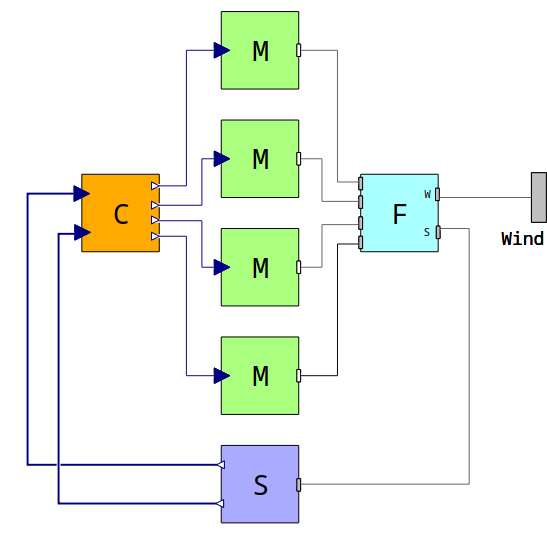
\includegraphics[width=100mm, keepaspectratio]{figures/stdSzim.png}
            \caption{A megkötések nélkül elkészített szimulációs modell.} 
            \label{fig:stdSzim}
        \end{figure}

        \subsubsection{FMI kompatibilis verzió}
        Ennek a modellnek a különlegessége, hogy míg az előzőben használható volt olyan kapcsolat, amely azt írta le, hogy a motorok fizikai kapcsolatban állnak a drón vázával, addig ebben a verzióban a komponensek határán csak logikai értékek valamint egész és racionális számok léphettek át.
        Ez persze feloldható volt a \ref{sec:fmiKompat} részben leírt módszerrel, azonban ennek következtében a motorok és a váz között nem egy mechanikai kapcsolat volt, amin a megfelelő értékek minkét irányba terjedhettek, hanem az adott motor keltette tolóerő és forgatónyomaték, amely a váz modelljén belül került átalakításra fizikai értékké. Ennek következtében az, hogy minden motor mozgása kihat a teljes rendszerre, csak úgy volt modellezhető, hogy a mozgásmodell teljesen a vázban került megvalósításra.

        Ennek kellemetlen következménye, hogy a motorok tömegét modellező blokkokat a vázban kellett elhelyezni, pedig ez egy külön alkatrész ami le is cserélhető egy másikra.
        Persze megoldható, hogy paraméterként adhassuk meg és az SSP (Lásd: \ref{sec:ssp} rész) szabvánnyal elméletben megoldható, hogy egy adott katalógusból választott motortípus kiválasztásával az egész modell átparaméterezhető legyen, de ez olyan komplex probléma ami nehezen automatizálható, sok hibalehetőséget tartalmaz és nehezen újrahasználható illetve karbantartható modellekhez vezet.

        Az, hogy egy komponens modellje részben egy másikba kerül áthelyezésre, és nem a valós kapcsolatokat látjuk, hanem számértékek terjedését, nagyban megnehezíti annak áttekintését és felhasználását, de cserébe megoldható a modellek átadása anélkül, hogy a gyártó felfedné az implementáció részleteit, ami több ipari résztvevő között gyakran megjelenő igény a közös munka során.
        Mindemellett amíg a szabványt nem bővítik a szükséges akauzális kapcsolatok leírásához szükséges megoldásokkal, addig ez a technika csak nagyon indokolt esetben javasolt.

        Az FMI kompatibilis modell a fentiekben leírt jelöléseknek megfelelően a \ref{fig:fmiSzim} ábrán látható.
        Megfigyelhető, hogy az előző modellhez képest itt kizárólag számadatok formájában áramlik adat a komponensek között.
        A szenzorok esetében a mérést végző blokkok a vázba kerültek és a \emph{Sensors} blokk csak a szenzorra jellemző zajt és egyéb paramétereket modellezi.
        A \emph{Motor} blokkok pedig kizárólag az általuk létrehozott mechanikai hatások mértékét továbbítja a váznak amely a teljes dinamikai modellt implementálja, beleértve a határain kívül eső blokkok szerepét is.

        \begin{figure}[!ht]
            \centering
            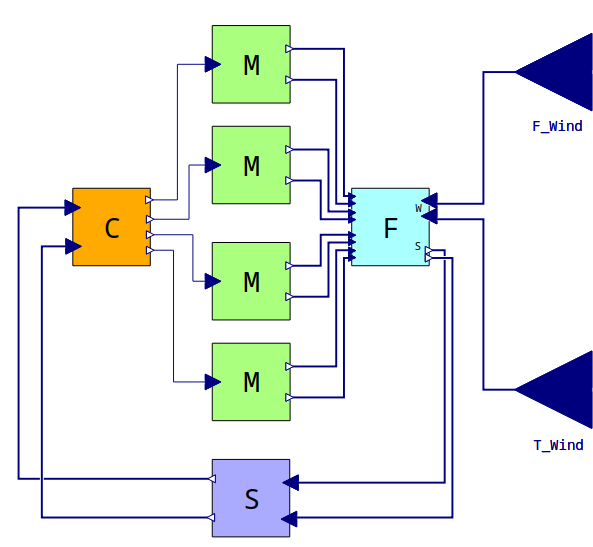
\includegraphics[width=100mm, keepaspectratio]{figures/fmiSzim.png}
            \caption{Az FMI szabvány megkötései szerint elkészített szimulációs modell.} 
            \label{fig:fmiSzim}
        \end{figure}

        \subsubsection{Szimulációs eredmények}
            \paragraph{Prototipizálás és validáció}
            A fejlesztés során a szimulációk segítségével választottam ki azokat a motorparamétereket, amelyekkel már megfelelő pontossággal garantálható volt a pozíciótartás.
            Az esettanulmány keretében ez azt jelentette, hogy minden méréshez manuálisan kellett átparaméterezni a szimulációs modellt és a gyűjtött adatokat manuálisan kiértékelni. Ez egy ilyen egyszerű példa keretében is időigényes feladat volt manuálisan, azonban nem igényelte  az összes motorvariáns és a többi alkatrész beszerzését és prototípusok gyártását, ahogy egy szélcsatorna használatát sem.

            A modellek automatikus generálásával ez a folyamat mindössze a mérési összeállítás és a követelmények modellezését tenné szükségessé, a mérések elvégzése és kiértékelése már teljesen automatizáltan történhetne, lehetővé téve több alternatíva gyors vizsgálatát.
            Fontos megemlíteni, hogy a követelmények és a mérési összeállítások modelljének egyébként is meg kell jelenni a rendszermodellben, mivel ez elengedhetetlen a nyomonkövethetőség biztosításához és a mérések megismételhetőségéhez.

            \paragraph{Végleges validáció}
            A fejlesztést befejezve, az utolsó lépés a végleges szimulációs modellek segítségével a modell validálása volt. A szimulációkat futtatva a rendszer mindkét modell esetében felemelkedett, megközelítette az előre kijelölt pozíciót és azt a széllökések mellett is tartotta elfogadható mértékű kitérések mellett.
            
            A szimulációs eredményeket szemléltető animációról készült képek a \ref{fig:SimRes} ábrán láthatóak.
            Az ábrán a fekete elemek a referencia koordináta-rendszert, a kékek magát a kvadkoptert, míg a zöldek az erőket és forgatónyomatékokat szemléltetik.
            A szélső, motorokat jelképező gömbökre hatóerők és forgatónyomatékok a motorok által keltettek, amelyekkel beavatkozunk a rendszerbe. Az origóból induló lefelé mutató erő a gravitációt reprezentálja.
            A kvadkopter testén ható erő és forgatónyomaték, amely az ábrán látható módon a többi nyíltól függetlenül mozog, a rendszerre ható szélzavarást reprezentálja.

            A szimuláció paraméterei úgy lettek meghatározva, hogy a rendszer az origóból felszállva az $y$ tengelyt jelképező nyíl hegyénél lebegjen.
            
            Az ábrán látható, hogy a rendszer a szimuláció második felében -öt másodperc után- már elérte a kitűzött célt, a továbbiakban ezt próbálja tartani a szélzavarás ellenére, ez okozza a harmadik és negyedik képen látható kitéréseket.
            Ezeknek az eredményeknek az alapján, a tervezési folyamat és az esettanulmány is sikeresnek tekinthető.

            \begin{figure}[!ht]
                \centering
                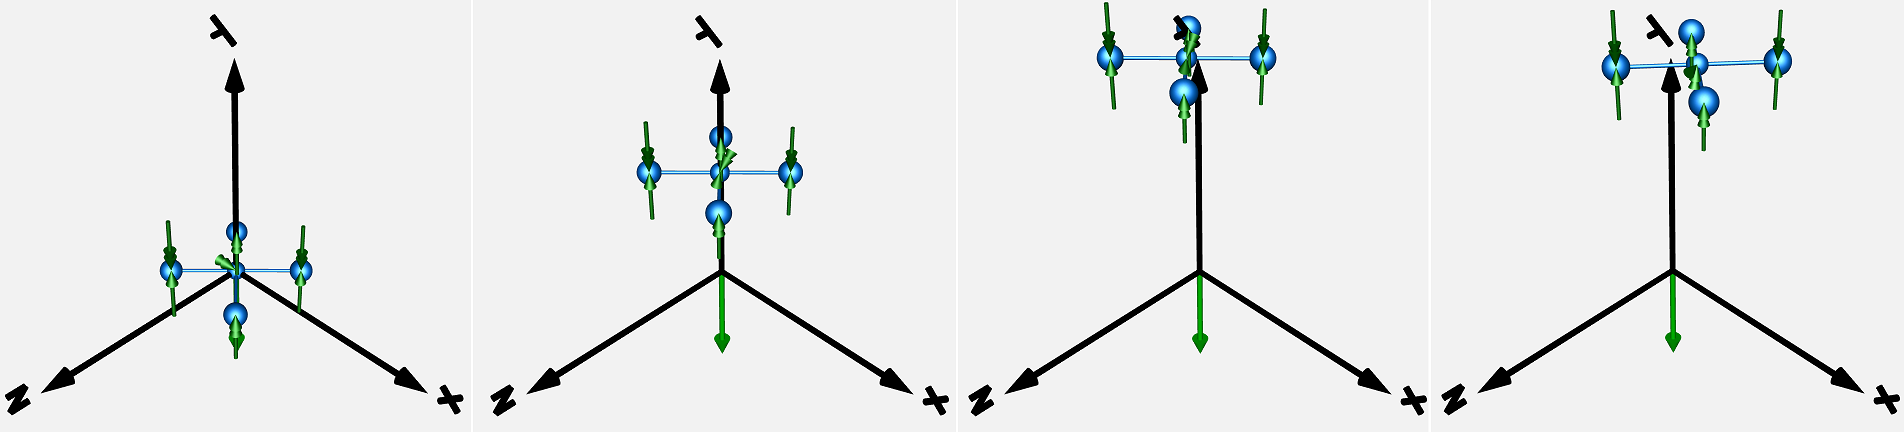
\includegraphics[width=150mm, keepaspectratio]{figures/SimRes.png}
                \caption{A szimulációk eredménye pillanatképeken.}
                \label{fig:SimRes}
            \end{figure}

    \section{Értékelés a motivációk szempontjából}
    Először érdemes megvizsgálni, hogy a dolgozat motivációjául szolgáló szempontok szerint mennyire eredményes az eddigi munka.

        \subsection{Rendszertervezési szempontok}
        A modellalapú technikák általános előnyei közzé tartozik a nyomonkövethetőség, a modellek konzisztenciája és a nézetek és dokumentumok automatikus generálhatósága.
        Mivel a dolgozatban javasolt módszertan is ilyen, modellalapú megközelítést alkalmaz, ezért ezeket nyelvi szinten teljesíti, illetve kompatibilis az eszközökkel amik képeset teljesíteni a konzisztencia esetében.
        A következő szempontok azok, amelyekre csupán lehetőséget biztosít a technológia, de ezek megvalósítása már a módszertannak köszönhető.

            \paragraph{Validáció és Verifikáció (V\&V) minden fejlesztési fázisban} \label{ertekelesVV}
            A módszertan bemutatása során látható volt, hogy a fejlesztés folyamán több alkalommal is szerepelnek validációs lépések, melyeknek célja a hibák mielőbbi kiszűrése.
            Ez komoly előrelépés a hagyományos módszerekhez és több modellalapú módszertanhoz képest, amelyek nem, vagy csak a fejlesztés végén tartalmaznak ilyen elemeket. (Lásd: \ref{sec:KorabbiModszerek} rész)
            Jelen dolgozat a szimulációs technológiákkal kapcsolatos validációra koncentrált, de természetesen ezekkel együtt végrehajthatóak más V\&V lépések is ugyanazokon a pontokon.

            \paragraph{Modellek újrahasználhatósága}
            A javasolt módszerek kitértek olyan könyvtárak használatára amelyek újrahasználhatóvá teszik az általános modellrészleteket.
            Ez a szempont jellemzően nem jelent meg az eddigi módszertanokban, bár természetesen nem is zárták ki ezek használatát. (Lásd: \ref{sec:KorabbiModszerek} rész)
            A javasolt megközelítés esetén kiemelendő, hogy a szimulációs technológiákkal integrált könyvtárakat javasol. Ezeknek a könyvtárba rendezése összhangban áll az általános szimulációs törekvésekkel és még inkább elősegíti a két terület integrálását.

        \subsection{Szimulációs szempontok}
        Mivel a módszertan lehetőséget nyújt a szimulációs technológiák alkalmazására, így magában foglalja azok előnyeit is.
        Meg kell említeni azonban, hogy bár a dolgozat kitért a HiL illetve SiL szimulációkkal való kompatibilitásra és elvi szinten támogatja azokat, ennek pontos megvalósításával nem volt lehetőség foglalkozni az eddigi munka során.

        \subsection{A két technológia integrálása szerint}
        Látható, hogy a kidolgozott módszerek számos előnnyel rendelkezik a két érintett terület kapcsán, azonban célja a kettő ötvözése, az alábbiakban egyesével értékelem az ennek kapcsán felmerült előrelépéseket és hiányosságokat.

            \paragraph{Szimulációs modellek automatikus generálása}
            Mivel a két terület integrálásához szükséges a rendszermodellben egy külön reprezentációt készíteni a szimulációs modellekhez, ezért felmerül az igény, hogy ezek alapján automatikusan állítsuk elő őket.
            
            A módszertan kidolgozása során részletesen vizsgáltam ezt a lehetőséget és kidolgozásra kerültek ennek alapvető sémái. Ezek az eredmények azért nem szerepeltek o dolgozatban, mert először későbbi fejlesztésre lettek félretéve, később pedig rábukkantam a \ref{sec:SysPhS} részben bemutatott SysPhS
            szabványra, amely az elérhető leírások alapján illeszkedik a kidolgozott alapelvekhez, így a saját megoldás helyett a két technológia ötvözése lett a cél ezen a területen.
            
            Az esettanulmány alatt, amikor a szimulációs modellreprezentációkat és a szimulációs modelleket is kézzel kellett elkészítenem, az eddigiek mellett felmerült, hogy magukat a modellreprezentációkat is lehetne részben automatikusan generálni, ezzel még jobban kiterjesztve ezeket az előnyöket.

            \paragraph{Munkafolyamatok konzisztenciájának garantálása}
            Az integrált technikák esetében ez a cél különböző modelltípusok konzisztenciáját jelenti. A módszertan javaslatot tett olyan modellstruktúrákra, amelyek megkönnyítik ennek ellenőrzését, illetve lehetőséget biztosít a kódgenerálásra, amely biztosítja ennek a konzisztenciának a felhasználóbarát megvalósítását is.
            
            Ami a szimulációk eredményeit illeti, ezeknek a garantált konzisztenciájához szükséges, hogy a szimuláció eredménye automatikusan visszakerüljön a rendszermodellbe.
            A leképezés ezen irányára nem tért ki a módszertan, bár az esettanulmány tapasztalatai alapján ez módszertantól független eszközökkel biztosítható, ha a tervezési folyamatban van hely ilyen vizsgálatoknak.
            A \ref{sec:flow} rész végén találhatóak javaslatok ilyen lépések elhelyezésére, így egy ilyen eszköz elméletileg gond nélkül használható a javasolt módszerekkel.

            \paragraph{Integrált V\&V}
            A két előző pont teljesülése esetén megvalósuló integrált V\&V folyamatok a fentiekben leírtak alapján elő lettek készítve, azonban tényleges megvalósításuk még várat magára, főleg mivel ehhez már szükség van az említett kétirányú kapcsolatra.
            
            \paragraph{Rendszer-identifikáció támogatása paraméter-visszavetítéssel}
            Ez a technológia ugyanarra a kétirányú kapcsolatra támaszkodik mint ami az előző két pontban is szerepelt, így ennek megvalósítása szintén külső eszközök fejlesztését igényli, de a tapasztalatok alapján, ha elkészülnek ilyen keretrendszerek, akkor azok használhatóak lesznek a leírt módszerekkel.

    \section{Értékelés a felhasználási tapasztalatok szerint}
    Az esettanulmány során készített modellek fejlesztésénél a leírt módszerek hatékonynak és kényelmesnek bizonyultak.
    
    A szimulációs modelltranszformáció alapvetően repetitív és monoton feladatnak bizonyultak, ahogy azt a \ref{sec:ReMoOsszehasonlitas} részben előrevetítettem, azonban ennek az elvégzése hosszútávon automatizálandó feladatként szerepelt a kezdetektől fogva.
    A tapasztalatok alapján ez a feladat valóban sematikus és jól automatizálható.
    
    A finomítások során szükséges adatok könnyen kinyerhetőek a javasolt allokáció-centrikus modellekből, nemcsak a tervezők, de az automatizált eszközök számára is. Mindkét eset megkönnyíthető lenne viszont nyelvi kiterjesztések használatával, amely érdekes továbbhaladási irányt jelent.
\chapter{Konklúzió és további munka}

\section{Összefoglalás}
A dolgozatban leírt munka során először összegyűjtöttem a modellalapú rendszertervezés és a szimulációs technológiák külön-külön illetve együttes alkalmazásának előnyeit.
Ezután megvizsgáltam egy, a fenti technikákat integráló SysML v2 alapú tervezési módszertan által teljesítendő követelményeket, javaslatot tettem több különböző implementációs irányra, majd kiértékeltem ezeket.

Az eredményeket felhasználva kidolgoztam ilyen módszertan alapjait és egy esettanulmányon keresztül demonstráltam az új, fentieknek megfelelő módszerek gyakorlati alkalmazását, ami számos az integrációból fakadó előnnyel jár, valamint alapot biztosít továbbiak elérésére, ha a hozzájuk szükséges fejlesztőeszközök létrejönnek.

A javasolt módszereknek három fontos eleme van, amelyek nem, vagy csak részlegesen jelennek meg a korábbi módszertanokban.
A dolgozat legfontosabb új gondolata az allokációk köré épülő rendszerszemlélet, amely a javasolt módszerek alapkövét képezi és tényleg különlegesnek számít a korábbi módszertanokhoz képest.
Ezután fontos megemlíteni a modell hierarchikus finomítását, amellyel jól elhatárolhatóak, a különböző absztrakciós szintjei a modellnek és kényelmesen teszi lehetővé különböző implementációs lehetőségek összehasonlítását. Ezt a megoldást SysML v2 új nyelvi elemeinek a felhasználása tette lehetővé.
Végül, de nem utolsó sorban, a javasolt megközelítésnek szerves részét képezik a szimulációs technikák. Erre a feladatra számos korábbi módszertanban tettek kísérletet, de azokban az esetekben mindig problémát jelentett, hogy ezeket utólag próbálták egy addigra kiforrott koncepcióba beilleszteni.

A munkám során feltárásra került, hogy a javasolt előnyök némelyike külön eszközöket igényel, amelyek csak a fejlesztési folyamatban igényelnek helyet a használatukhoz, magától az alkalmazott módszertantól függetlenek.
Ezek esetében megvizsgáltam, hogy használhatóak-e ezek a technikák a javasolt megközelítésekkel, melynek során nem találtam kizáró okot az együttes használatra.

\section{További kutatási és fejlesztési lehetőségek}
A rendszertervezési módszertanokban (Lásd: \ref{sec:KorabbiModszerek} rész) rendszerint a rendszer modellezése mellett nagy hangsúlyt helyeznek annak kontextusának, azaz beágyazó környezetének a modellezésére. Sajnos az eddigi munkám során ezt nem volt még lehetőségem kidolgozni, ezért szeretném először ezt a hiányosságát pótolni a javasolt módszertannak, hogy minél közelebb kerüljön egy teljes, gyakorlatban is jól alkalmazható módszertanhoz.

A kódgenerálás kapcsán felmerült, hogy ez az elem elengedhetetlen ahhoz, hogy egy módszertan megfeleljen eredeti rendeltetésének, és bemutatásra került a fejlesztés alatt álló SysPhS szabvány is, amely alkalmazásával ez a feladat gyorsabban megoldható, mint saját eszköz fejlesztésével.
Ezek alapján konzulensemmel fel is vettük a kapcsolatot a szabványon dolgozó egyik csapattal és megkezdtük az együttműködést a két eszköz összekapcsolása érdekében.

Jelen dolgozat elsődlegesen a validációs technológiák közül a szimulációk integrálásával foglalkozott, mert ezek igényelnek külön környezetekben készített és futtatott modelleket, azonban a jövőben szeretnék több, más V\&V technikát is integrálni a javasolt módszerekbe és ezek függvényében bővíteni a bemutatott esettanulmányt.
Az esettanulmány kidolgozása folyamán az eddig kidolgozott módszerekben azonosítottam több általános mintát, melyeknek egy SysML v2 nyelvi kiterjesztésben való összegyűjtése tovább egyszerűsítené azok használatát, amely előnyös lenne egy teljes módszertan kidolgozása esetén. Természetesen a nyelvi kiterjesztés elkészültével újra frissíteném az esettanulmányt, hogy használható legyen az új, kiforrottabb módszerek bemutatására, valamint referenciamodellnek.

%%TMP
%%----------------------------------------------------------------------------
\chapter{\bevezetes}
%----------------------------------------------------------------------------

A bevezető tartalmazza a diplomaterv-kiírás elemzését, történelmi előzményeit, a feladat indokoltságát (a motiváció leírását), az eddigi megoldásokat, és ennek tükrében a hallgató megoldásának összefoglalását.

A bevezető szokás szerint a diplomaterv felépítésével záródik, azaz annak rövid leírásával, hogy melyik fejezet mivel foglalkozik.

%%----------------------------------------------------------------------------
\chapter{\LaTeX-eszközök}
\label{sec:LatexTools}
%----------------------------------------------------------------------------
\section{A szerkesztéshez használatos eszközök}
%----------------------------------------------------------------------------
Ez a sablon TeXstudio 2.8.8 szerkesztővel készült. A TeXstudio egy platformfüggetlen, Windows, Linux és Mac OS alatt is elérhető \LaTeX-szerkesztőprogram számtalan hasznos szolgáltatással (\refstruc{fig:TeXstudio}). A szoftver ingyenesen letölthető\footnote{A TeXstudio hivatalos oldala: \url{http://texstudio.sourceforge.net/}}.

\begin{figure}[!ht]
\centering
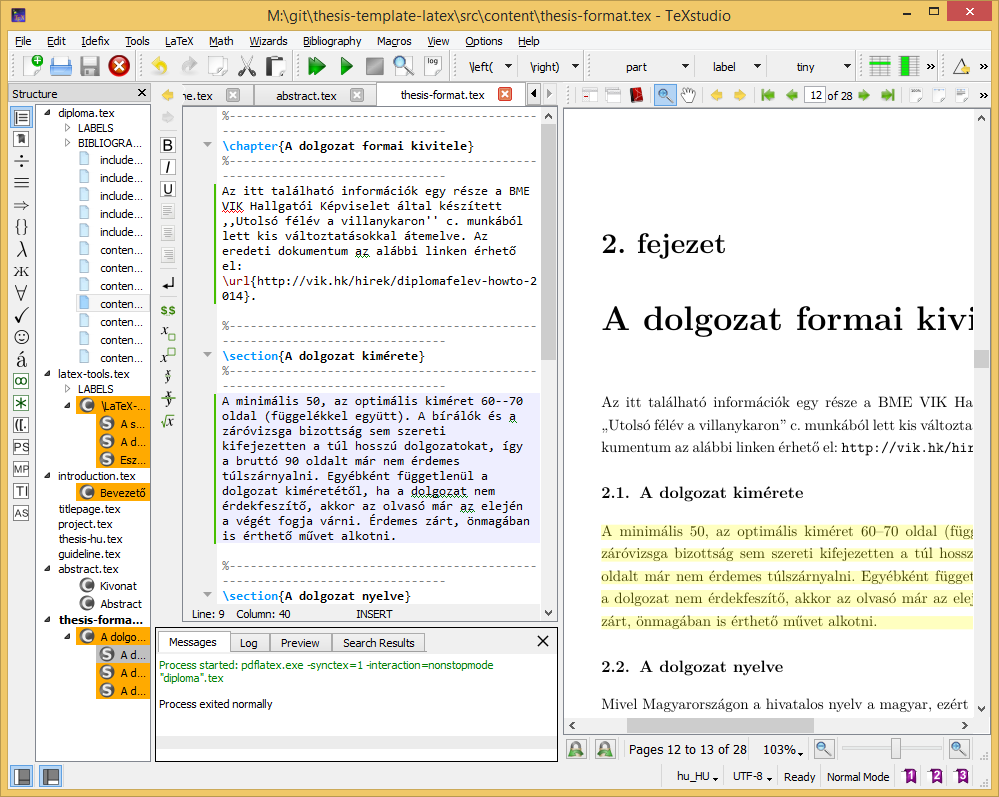
\includegraphics[width=150mm, keepaspectratio]{figures/TeXstudio.png}
\caption{A TeXstudio \LaTeX-szerkesztő.}
\label{fig:TeXstudio}
\end{figure}

A TeXstudio telepítése után érdemes még letölteni a magyar nyelvű helyesírásellenőrző-szótárakat hozzá. A TeXstudio az OpenOffice-hoz használatos formátumot tudja kezelni. A TeXstudio beállításainál a \verb+General+ fülön a \verb+Dictionaries+ résznél tudjuk megadni, hogy melyik szótárat használja.

Egy másik használható Windows alapú szerkesztőprogram a LEd\footnote{A LEd hivatalos oldala: \url{http://www.latexeditor.org/}} (LaTeX Editor), a TeXstudio azonban stabilabb, gyorsabb, és jobban használható.

%----------------------------------------------------------------------------
\section{A dokumentum lefordítása Windows alatt}
%----------------------------------------------------------------------------
A TeXstudio és a LEd kizárólag szerkesztőprogram (bár az utóbbiban DVI-nézegető is van), így a dokumentum fordításához szükséges eszközöket nem tartalmazza. Windows alatt alapvetően két lehetőség közül érdemes választani: MiKTeX (\url{http://miktex.org/}) és TeX Live (\url{http://www.tug.org/texlive/}) programcsomag. Az utóbbi működik Mac OS X, GNU/Linux alatt és Unix-származékokon is. A MiKTeX egy alapcsomag telepítése után mindig letölti a használt funkciókhoz szükséges, de lokálisan hiányzó \TeX-csomagokat, míg a TeX Live DVD ISO verzóban férhető hozzá. Ez a dokumentum TeX Live 2008 programcsomag segítségével fordult, amelynek DVD ISO verziója a megadott oldalról letölthető. A sablon lefordításához a disztribúcióban szereplő \verb+magyar.ldf+ fájlt a \verb+http://www.math.bme.hu/latex/+ változatra kell cserélni, vagy az utóbbi változatot be kell másolni a projekt-könyvtárba (ahogy ezt meg is tettük a sablonban) különben anomáliák tapasztalhatók a dokumentumban (pl. az ábra- és táblázat-aláírások formátuma nem a beállított lesz, vagy bizonyos oldalakon megjelenik alapértelmezésben egy fejléc). A TeX Live 2008-at még nem kell külön telepíteni a gépre, elegendő DVD-ről (vagy az ISO fájlból közvetlenül, pl. DaemonTools-szal) használni.

Ha a MiKTeX csomagot használjuk, akkor parancssorból a következő módon tudjuk újrafordítani a teljes dokumentumot:

\begin{lstlisting}[language=bash,frame=single,float=!ht]
$ texify -p thesis.tex
\end{lstlisting}

A \verb+texify+ parancs a MiKTex programcsomag \verb+miktex/bin+ alkönyvtárában található. A parancs gondoskodik arról, hogy a szükséges lépéseket (fordítás, hivatkozások generálása stb.) a megfelelő sorrendben elvégezze. A \verb+-p+ kapcsoló hatására PDF-et generál. A fordítást és az ideiglenes fájlok törlését elvégezhetjük a sablonhoz mellékelt \verb+manual_build.bat+ szkript segítségével is.

A \TeX-eszközöket tartalmazó programcsomag binárisainak elérési útját gyakran be kell állítani a szerkesztőprogramban, például TeXstudio esetén legegyszerűbben az \verb+Options / Configure TeXstudio... / Commands+ menüponttal előhívott dialógusablakban tehetjük ezt meg.

A PDF-\LaTeX~használata esetén a generált dokumentum közvetlenül PDF-formátumban áll rendelkezésre. Amennyiben a PDF-fájl egy PDF-nézőben (pl. Adobe Acrobat Reader vagy Foxit PDF Reader) meg van nyitva, akkor a fájlleírót a PDF-néző program tipikusan lefoglalja. Ilyen esetben a dokumentum újrafordítása hibaüzenettel kilép. Ha bezárjuk és újra megnyitjuk a PDF dokumentumot, akkor pedig a PDF-nézők többsége az első oldalon nyitja meg a dokumentumot, nem a legutóbb olvasott oldalon. Ezzel szemben például az egyszerű és ingyenes \textcolor{blue}{Sumatra PDF} nevű program képes arra, hogy a megnyitott dokumentum megváltozását detektálja, és frissítse a nézetet az aktuális oldal megtartásával.

%----------------------------------------------------------------------------
\section{Eszközök Linuxhoz}
%----------------------------------------------------------------------------
Linux operációs rendszer alatt is rengeteg szerkesztőprogram van, pl. a KDE alapú Kile jól használható. Ez ingyenesen letölthető, vagy éppenséggel az adott Linux-disztribúció eleve tartalmazza, ahogyan a dokumentum fordításához szükséges csomagokat is. Az Ubuntu Linux disztribúciók alatt például legtöbbször a \verb+texlive-*+ csomagok telepítésével használhatók a \LaTeX-eszközök. A jelen sablon fordításához szükséges csomagok (kb. 0,5 GB) az alábbi paranccsal telepíthetők:

\begin{lstlisting}[language=bash,morekeywords={sudo,apt\-get},alsoletter={-},breaklines=true]
$ sudo apt-get install texlive-latex-extra texlive-fonts-extra texlive-fonts-recommended texlive-lang-european texlive-xetex texlive-science
\end{lstlisting}

Amennyiben egy újabb csomag hozzáadása után hiányzó fájlra utaló hibát kapunk a fordítótól, telepítenünk kell az azt tartalmazó TeX Live csomagot. Ha pl. a \verb+bibentry+ csomagot szeretnénk használni, futtassuk az alábbi parancsot:

\begin{lstlisting}[language=bash,morekeywords={apt\-cache},alsoletter={-},breaklines=true]
$ apt-cache search bibentry
texlive-luatex - TeX Live: LuaTeX packages
\end{lstlisting}

Majd telepítsük fel a megfelelő TeX Live csomagot, jelen esetben a `texlive-lualatex`-et. (Egy LaTeX csomag több TeX Live csomagban is szerepelhet.)

Ha gyakran szerkesztünk más \LaTeX dokumentumokat is, kényelmes és biztos megoldás a teljes TeX Live disztribúció telepítése, ez azonban kb. 4 GB helyet igényel.

\begin{lstlisting}[language=bash,morekeywords={sudo,apt\-get},alsoletter={-},breaklines=true]
sudo apt-get install texlive-full
\end{lstlisting}

%%----------------------------------------------------------------------------
\chapter{A dolgozat formai kivitele}
%----------------------------------------------------------------------------
Az itt található információk egy része a BME VIK Hallgatói Képviselet által készített ,,Utolsó félév a villanykaron'' c. munkából lett kis változtatásokkal átemelve. Az eredeti dokumentum az alábbi linken érhető el: \url{http://vik.hk/hirek/diplomafelev-howto-2015}.

%----------------------------------------------------------------------------
\section{A dolgozat kimérete}
%----------------------------------------------------------------------------
Szakdolgozat esetében minimum 30, 45 körüli ajánlott oldalszám lehet az iránymutató. De mindenképp érdemes rákérdezni a konzulensnél is az elvárásokra, mert tanszékenként változóak lehetnek az elvárások.

Mesterképzésen a Diplomatervezés 1 esetében a beszámoló még inkább az Önálló laboratóriumi beszámolókhoz hasonlít, tanszékenként eltérő formai követelményekkel, -- egy legalább 30 oldal körüli dolgozat az elvárt -- és az elmúlt fél éves munkáról szól. De egyben célszerű, ha ez a végleges diplomaterv alapja is. (A végleges 60-90 oldal körülbelül a hasznos részre nézve)


%----------------------------------------------------------------------------
\section{A dolgozat nyelve}
%----------------------------------------------------------------------------
Mivel Magyarországon a hivatalos nyelv a magyar, ezért alapértelmezésben magyarul kell megírni a dolgozatot. Aki külföldi posztgraduális képzésben akar részt venni, nemzetközi szintű tudományos kutatást szeretne végezni, vagy multinacionális cégnél akar elhelyezkedni, annak célszerű angolul megírnia diplomadolgozatát. Mielőtt a hallgató az angol nyelvű verzió mellett dönt, erősen ajánlott mérlegelni, hogy ez mennyi többletmunkát fog a hallgatónak jelenteni fogalmazás és nyelvhelyesség terén, valamint -- nem utolsó sorban -- hogy ez mennyi többletmunkát fog jelenteni a konzulens illetve bíráló számára. Egy nehezen olvasható, netalán érthetetlen szöveg teher minden játékos számára.

%----------------------------------------------------------------------------
\section{A dokumentum nyomdatechnikai kivitele}
%----------------------------------------------------------------------------
A dolgozatot A4-es fehér lapra nyomtatva, 2,5 centiméteres margóval (+1~cm kötésbeni), 11--12 pontos betűmérettel, talpas betűtípussal és egyszeres sorközzel célszerű elkészíteni.
A másfeles sorköz (\verb+\onehalfspacing+ beállítás) is elfogadott szakdolgozatokban és diplomamunkákban, de ajánlott megtartani az egyszeres sorközt.

Annak érdekében, hogy a dolgozat külsőleg is igényes munka benyomását keltse, érdemes figyelni az alapvető tipográfiai szabályok betartására~\cite{Jeney}.

%% !TeX spellcheck = hu_HU
% !TeX encoding = UTF-8
% !TeX program = xelatex
%----------------------------------------------------------------------------
\chapter{A \LaTeX-sablon használata}
%----------------------------------------------------------------------------

Ebben a fejezetben röviden, implicit módon bemutatjuk a sablon használatának módját, ami azt jelenti, hogy sablon használata ennek a dokumentumnak a forráskódját tanulmányozva válik teljesen világossá. Amennyiben a szoftver-keretrendszer telepítve van, a sablon alkalmazása és a dolgozat szerkesztése \LaTeX-ben a sablon segítségével tapasztalataink szerint jóval hatékonyabb, mint egy WYSWYG (\emph{What You See is What You Get}) típusú szövegszerkesztő esetén (pl. Microsoft Word, OpenOffice).

%----------------------------------------------------------------------------
\section{Címkék és hivatkozások}
%----------------------------------------------------------------------------
A \LaTeX~dokumentumban címkéket (\verb+\label+) rendelhetünk ábrákhoz, táblázatokhoz, fejezetekhez, listákhoz, képletekhez stb. Ezekre a dokumentum bármely részében hivatkozhatunk, a hivatkozások automatikusan feloldásra kerülnek.

A sablonban makrókat definiáltunk a hivatkozások megkönnyítéséhez. Ennek megfelelően minden ábra (\emph{figure}) címkéje \verb+fig:+ kulcsszóval kezdődik, míg minden táblázat (\emph{table}), képlet (\emph{equation}), fejezet (\emph{section}) és lista (\emph{listing}) rendre a \verb+tab:+, \verb+eq:+, \verb+sec:+ és \verb+lst:+ kulcsszóval kezdődik, és a kulcsszavak után tetszőlegesen választott címke használható. Ha ezt a konvenciót betartjuk, akkor az előbbi objektumok számára rendre a \verb+\figref+, \verb+\tabref+, \verb+\eqref+, \verb+\sectref+ és \verb+\listref+ makrókkal hivatkozhatunk. A makrók paramétere a címke, amelyre hivatkozunk (a kulcsszó nélkül). Az összes említett hivatkozástípus, beleértve az \verb+\url+ kulcsszóval bevezetett web-hivatkozásokat is a  \verb+hyperref+\footnote{Segítségével a dokumentumban megjelenő hivatkozások nem csak dinamikussá válnak, de színezhetők is, bővebbet erről a csomag dokumentációjában találunk. Ez egyúttal egy példa lábjegyzet írására.} csomagnak köszönhetően aktívak a legtöbb PDF-nézegetőben, rájuk kattintva a dokumentum megfelelő oldalára ugrik a PDF-néző vagy a megfelelő linket megnyitja az alapértelmezett böngészővel. A \verb+hyperref+ csomag a kimeneti PDF-dokumentumba könyvjelzőket is készít a tartalomjegyzékből. Ez egy szintén aktív tartalomjegyzék, amelynek elemeire kattintva a nézegető behozza a kiválasztott fejezetet.

%----------------------------------------------------------------------------
\section{Ábrák és táblázatok}
%----------------------------------------------------------------------------
Használjunk vektorgrafikus ábrákat, ha van rá módunk. PDFLaTeX használata esetén PDF formátumú ábrákat lehet beilleszteni könnyen, az EPS (PostScript) vektorgrafikus képformátum beillesztését a PDFLaTeX közvetlenül nem támogatja (de lehet konvertálni, lásd később). Ha vektorgrafikus formában nem áll rendelkezésünkre az ábra, akkor a  veszteségmentes PNG, valamint a veszteséges JPEG formátumban érdemes elmenteni.  Figyeljünk arra, hogy ilyenkor a képek felbontása elég nagy legyen ahhoz, hogy nyomtatásban is megfelelő minőséget nyújtson (legalább 300 dpi javasolt). A dokumentumban felhasznált képfájlokat a dokumentum forrása mellett érdemes tartani, archiválni, mivel ezek hiányában a dokumentum nem fordul újra. Ha lehet, a vektorgrafikus képeket vektorgrafikus formátumban is érdemes elmenteni az újrafelhasználhatóság (az átszerkeszthetőség) érdekében.

Kapcsolási rajzok legtöbbször kimásolhatók egy vektorgrafikus programba (pl. CorelDraw) és onnan nagyobb felbontással raszterizálva kimenthatők PNG formátumban. Ugyanakkor kiváló ábrák készíthetők Microsoft Visio vagy hasonló program használatával is: Visio-ból az ábrák közvetlenül PDF-be is menthetők.

Lehetőségeink Matlab ábrák esetén:
\begin{itemize}
	\item Képernyőlopás (\emph{screenshot}) is elfogadható minőségű lehet a dokumentumban, de általában jobb felbontást is el lehet érni más módszerrel.
	\item A Matlab ábrát a \verb+File/Save As+ opcióval lementhetjük PNG formátumban (ugyanaz itt is érvényes, mint korábban, ezért nem javasoljuk).
	\item A Matlab ábrát az \verb+Edit/Copy figure+ opcióval kimásolhatjuk egy vektorgrafikus programba is és onnan nagyobb felbontással raszterizálva kimenthatjük PNG formátumban (nem javasolt).
	\item Javasolt megoldás: az ábrát a \verb+File/Save As+ opcióval EPS \emph{vektorgrafikus} formátumban elmentjük, PDF-be konvertálva beillesztjük a dolgozatba.
\end{itemize}
Az EPS kép az \verb+epstopdf+ programmal\footnote{a korábban említett \LaTeX-disztribúciókban megtalálható} konvertálható PDF formátumba. Célszerű egy batch-fájlt készíteni az összes EPS ábra lefordítására az alábbi módon (ez Windows alatt működik).
\begin{lstlisting}[language=]
@echo off
for %%j in (*.eps) do (
  echo converting file "%%j"
  epstopdf "%%j"
)
echo done .
\end{lstlisting}

Egy ilyen parancsfájlt (\verb+convert.cmd+) elhelyeztük a sablon \verb+figures\eps+ könyvtárába, így a felhasználónak csak annyi a dolga, hogy a \verb+figures\eps+ könyvtárba kimenti az EPS formátumú vektorgrafikus képet, majd lefuttatja a \verb+convert.cmd+ parancsfájlt, ami PDF-be konvertálja az EPS fájlt.

Ezek után a PDF-ábrát ugyanúgy lehet a dokumentumba beilleszteni, mint a PNG-t vagy a JPEG-et. A megoldás előnye, hogy a lefordított dokumentumban is vektorgrafikusan tárolódik az ábra, így a mérete jóval kisebb, mintha raszterizáltuk volna beillesztés előtt. Ez a módszer minden -- az EPS formátumot ismerő -- vektorgrafikus program (pl. CorelDraw) esetén is használható.

A képek beillesztésére \az+\refstruc{sec:LatexTools}ben mutattunk be példát (\refstruc{fig:TeXstudio}). Az előző mondatban egyúttal az automatikusan feloldódó ábrahivatkozásra is láthatunk példát. Több képfájlt is beilleszthetünk egyetlen ábrába. Az egyes képek közötti horizontális és vertikális margót metrikusan szabályozhatjuk (\refstruc{fig:HVSpaces}). Az ábrák elhelyezését számtalan tipográfiai szabály egyidejű teljesítésével a fordító maga végzi, a dokumentum írója csak preferenciáit jelezheti a fordító felé (olykor ez bosszúságot is okozhat, ilyenkor pl. a kép méretével lehet játszani).

\begin{figure}[!ht]
	\centering
	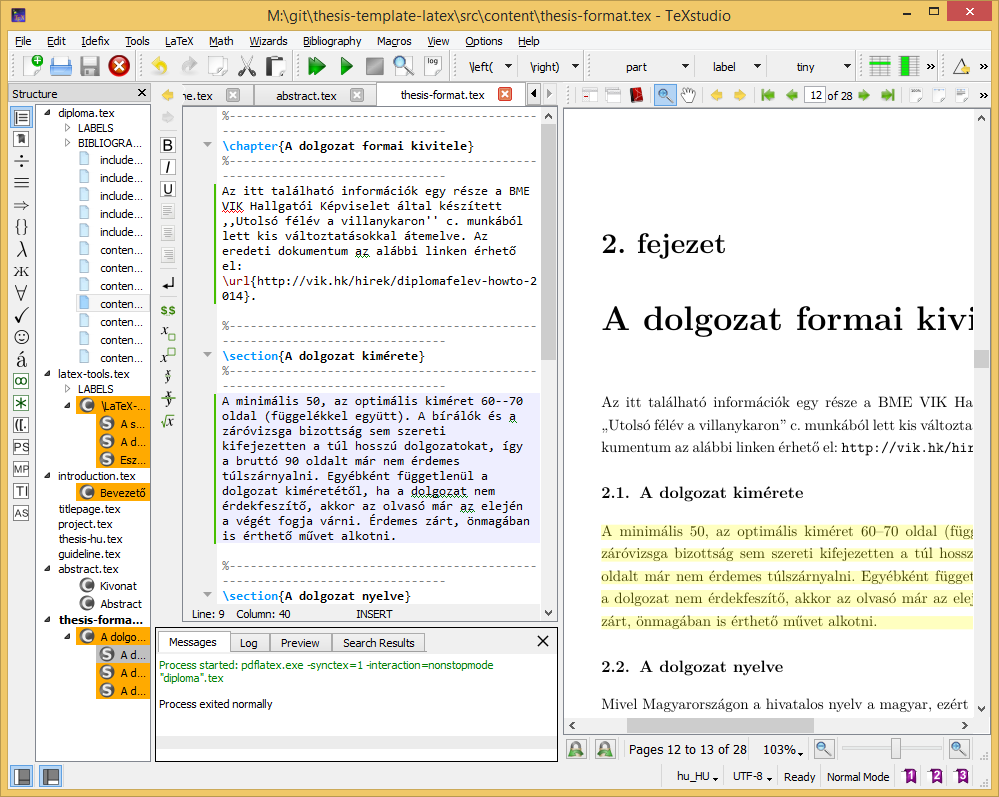
\includegraphics[width=67mm, keepaspectratio]{figures/TeXstudio.png}\hspace{1cm}
	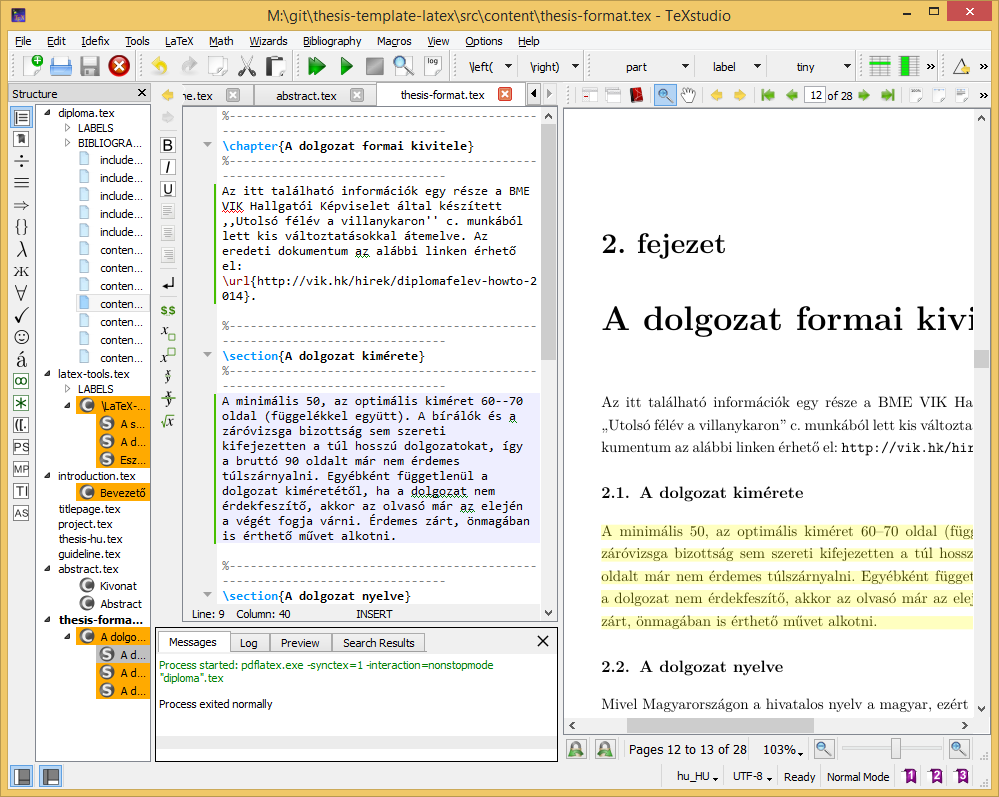
\includegraphics[width=67mm, keepaspectratio]{figures/TeXstudio.png}\\\vspace{5mm}
	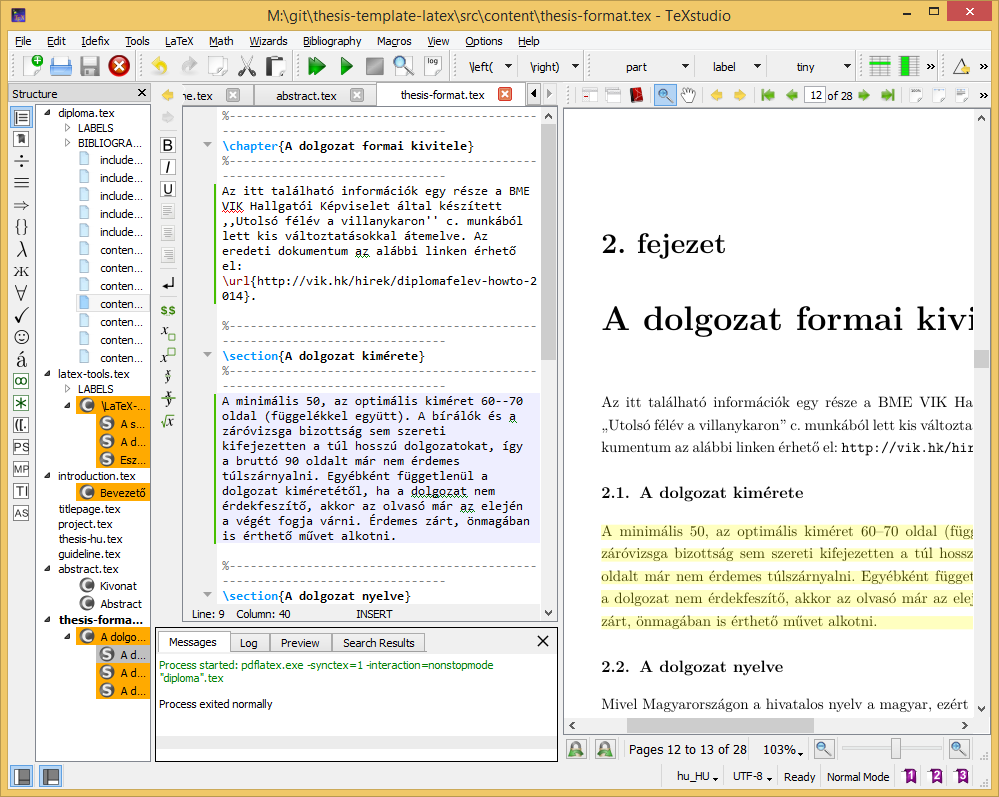
\includegraphics[width=67mm, keepaspectratio]{figures/TeXstudio.png}\hspace{1cm}
	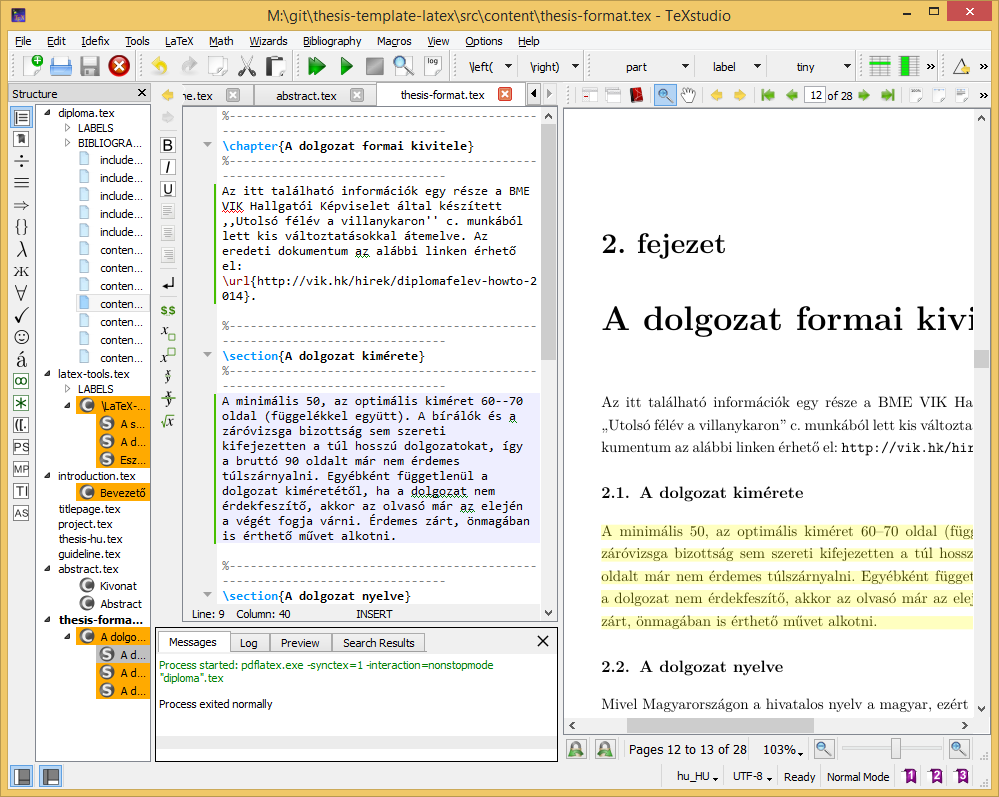
\includegraphics[width=67mm, keepaspectratio]{figures/TeXstudio.png}
	\caption{Több képfájl beillesztése esetén térközöket is érdemes használni.}
	\label{fig:HVSpaces}
\end{figure}

A táblázatok használatára \aref{tab:TabularExample}~táblázat mutat példát. A táblázatok formázásához hasznos tanácsokat találunk a \verb+booktabs+ csomag dokumentációjában.

\begin{table}[ht]
	\footnotesize
	\centering
	\begin{tabular}{ l c c }
		\toprule
		Órajel & Frekvencia & Cél pin \\
		\midrule
		CLKA & 100 MHz & FPGA CLK0\\
		CLKB & 48 MHz  & FPGA CLK1\\
		CLKC & 20 MHz  & Processzor\\
		CLKD & 25 MHz  & Ethernet chip \\
		CLKE & 72 MHz  & FPGA CLK2\\
		XBUF & 20 MHz  & FPGA CLK3\\
		\bottomrule
	\end{tabular}
	\caption{Az órajel-generátor chip órajel-kimenetei.}
	\label{tab:TabularExample}
\end{table}


%----------------------------------------------------------------------------
\section{Felsorolások és listák}
%----------------------------------------------------------------------------
Számozatlan felsorolásra mutat példát a jelenlegi bekezdés:
\begin{itemize}
	\item \emph{első bajusz:} ide lehetne írni az első elem kifejését,
	\item \emph{második bajusz:} ide lehetne írni a második elem kifejését,
	\item \emph{ez meg egy szakáll:} ide lehetne írni a harmadik elem kifejését.
\end{itemize}

Számozott felsorolást is készíthetünk az alábbi módon:
\begin{enumerate}
	\item \emph{első bajusz:} ide lehetne írni az első elem kifejését, és ez a kifejtés így néz ki, ha több sorosra sikeredik,
	\item \emph{második bajusz:} ide lehetne írni a második elem kifejését,
	\item \emph{ez meg egy szakáll:} ide lehetne írni a harmadik elem kifejését.
\end{enumerate}
A felsorolásokban sorok végén vessző, az utolsó sor végén pedig pont a szokásos írásjel. Ez alól kivételt képezhet, ha az egyes elemek több teljes mondatot tartalmaznak.

Listákban a dolgozat szövegétől elkülönítendő kódrészleteket, programsorokat, pszeudo-kódokat jeleníthetünk meg (\ref{lst:Example}.~kódrészlet).
\begin{lstlisting}[language=tex,caption=A fenti számozott felsorolás \LaTeX-forráskódja,label=lst:Example]
\begin{enumerate}
	\item \emph{els(*@ő@*) bajusz:} ide lehetne írni az els(*@ő@*) elem kifejését,
	és ez a kifejtés így néz ki, ha több sorosra sikeredik,
	\item \emph{második bajusz:} ide lehetne írni a második elem kifejését,
	\item \emph{ez meg egy szakáll:} ide lehetne írni a harmadik elem kifejését.
\end{enumerate}
\end{lstlisting}
A lista keretét, háttérszínét, egész stílusát megválaszthatjuk. Ráadásul különféle programnyelveket és a nyelveken belül kulcsszavakat is definiálhatunk, ha szükséges. Erről bővebbet a \verb+listings+ csomag hivatalos leírásában találhatunk.

%----------------------------------------------------------------------------
\section{Képletek}
%----------------------------------------------------------------------------
Ha egy formula nem túlságosan hosszú, és nem akarjuk hivatkozni a szövegből, mint például a $e^{i\pi}+1=0$ képlet, \emph{szövegközi képletként} szokás leírni. Csak, hogy másik példát is lássunk, az $U_i=-d\Phi/dt$ Faraday-törvény a $\rot E=-\frac{dB}{dt}$ differenciális alakban adott Maxwell-egyenlet felületre vett integráljából vezethető le. Látható, hogy a \LaTeX-fordító a sorközöket betartja, így a szöveg szedése esztétikus marad szövegközi képletek használata esetén is.

Képletek esetén az általános konvenció, hogy a kisbetűk skalárt, a kis félkövér betűk ($\mathbf{v}$) oszlopvektort -- és ennek megfelelően $\mathbf{v}^T$ sorvektort -- a kapitális félkövér betűk ($\mathbf{V}$) mátrixot jelölnek. Ha ettől el szeretnénk térni, akkor az alkalmazni kívánt jelölésmódot célszerű külön alfejezetben definiálni. Ennek megfelelően, amennyiben $\mathbf{y}$ jelöli a mérések vektorát, $\mathbf{\vartheta}$ a paraméterek vektorát és $\hat{\mathbf{y}}=\mathbf{X}\vartheta$ a paraméterekben lineáris modellt, akkor a \emph{Least-Squares} értelemben optimális paraméterbecslő $\hat{\mathbf{\vartheta}}_{LS}=(\mathbf{X}^T\mathbf{X})^{-1}\mathbf{X}^T\mathbf{y}$ lesz.

Emellett kiemelt, sorszámozott képleteket is megadhatunk, ennél az \verb+equation+ és a \verb+eqnarray+ környezetek helyett a korszerűbb \verb+align+ környezet alkalmazását javasoljuk (több okból, különféle problémák elkerülése végett, amelyekre most nem térünk ki). Tehát
\begin{align}
\dot{\mathbf{x}}&=\mathbf{A}\mathbf{x}+\mathbf{B}\mathbf{u},\\
\mathbf{y}&=\mathbf{C}\mathbf{x},
\end{align}
ahol $\mathbf{x}$ az állapotvektor, $\mathbf{y}$ a mérések vektora és $\mathbf{A}$, $\mathbf{B}$ és $\mathbf{C}$ a rendszert leíró paramétermátrixok. Figyeljük meg, hogy a két egyenletben az egyenlőségjelek egymáshoz igazítva jelennek meg, mivel a mindkettőt az \& karakter előzi meg a kódban. Lehetőség van számozatlan kiemelt képlet használatára is, például
\begin{align}
\dot{\mathbf{x}}&=\mathbf{A}\mathbf{x}+\mathbf{B}\mathbf{u},\nonumber\\
\mathbf{y}&=\mathbf{C}\mathbf{x}\nonumber.
\end{align}
Mátrixok felírására az $\mathbf{A}\mathbf{x}=\mathbf{b}$ inhomogén lineáris egyenlet részletes kifejtésével mutatunk példát:
\begin{align}
\begin{bmatrix}
a_{11} & a_{12} & \dots & a_{1n}\\
a_{21} & a_{22} & \dots & a_{2n}\\
\vdots & \vdots & \ddots & \vdots\\
a_{m1} & a_{m2} & \dots & a_{mn}
\end{bmatrix}
\begin{pmatrix}x_1\\x_2\\\vdots\\x_n\end{pmatrix}=
\begin{pmatrix}b_1\\b_2\\\vdots\\b_m\end{pmatrix}.
\end{align}
A \verb+\frac+ utasítás hatékonyságát egy általános másodfokú tag átviteli függvényén keresztül mutatjuk be, azaz
\begin{align}
W(s)=\frac{A}{1+2T\xi s+s^2T^2}.
\end{align}
A matematikai mód minden szimbólumának és képességének a bemutatására természetesen itt nincs lehetőség, de gyors referenciaként hatékonyan használhatók a következő linkek:\\
\indent\url{http://www.artofproblemsolving.com/LaTeX/AoPS_L_GuideSym.php},\\
\indent\url{http://www.ctan.org/tex-archive/info/symbols/comprehensive/symbols-a4.pdf},\\
\indent\url{ftp://ftp.ams.org/pub/tex/doc/amsmath/short-math-guide.pdf}.\\
Ez pedig itt egy magyarázat, hogy miért érdemes \verb+align+ környezetet használni:\\
\indent\url{http://texblog.net/latex-archive/maths/eqnarray-align-environment/}.

%----------------------------------------------------------------------------
\section{Irodalmi hivatkozások}
\label{sec:HowtoReference}
%----------------------------------------------------------------------------
Egy \LaTeX~dokumentumban az irodalmi hivatkozások definíciójának két módja van. Az egyik a \verb+\thebibliograhy+ környezet használata a dokumentum végén, az \verb+\end{document}+ lezárás előtt.
\begin{lstlisting}[language=tex]
\begin{thebibliography}{9}

\bibitem{Lamport94} Leslie Lamport, \emph{\LaTeX: A Document Preparation System}.
Addison Wesley, Massachusetts, 2nd Edition, 1994.

\end{thebibliography}
\end{lstlisting}

Ezek után a dokumentumban a \verb+\cite{Lamport94}+ utasítással hivatkozhatunk a forrásra. A fenti megadás viszonylag kötetlen, a szerző maga formázza az irodalomjegyzéket (ami gyakran inkonzisztens eredményhez vezet).

Egy sokkal professzionálisabb módszer a BiB\TeX{} használata, ezért ez a sablon is ezt támogatja. Ebben az esetben egy külön szöveges adatbázisban definiáljuk a forrásmunkákat, és egy külön stílusfájl határozza meg az irodalomjegyzék kinézetét. Ez, összhangban azzal, hogy külön formátumkonvenció határozza meg a folyóirat-, a könyv-, a konferenciacikk- stb. hivatkozások kinézetét az irodalomjegyzékben (a sablon használata esetén ezzel nem is kell foglalkoznia a hallgatónak, de az eredményt célszerű ellenőrizni). felhasznált hivatkozások adatbázisa egy \verb+.bib+ kiterjesztésű szöveges fájl, amelynek szerkezetét a \Aref{lst:Bibtex} kódrészlet demonstrálja. A forrásmunkák bevitelekor a sor végi vesszők külön figyelmet igényelnek, mert hiányuk a BiB\TeX-fordító hibaüzenetét eredményezi. A forrásmunkákat típus szerinti kulcsszó vezeti be (\verb+@book+ könyv, \verb+@inproceedings+ konferenciakiadványban megjelent cikk, \verb+@article+ folyóiratban megjelent cikk, \verb+@techreport+ valamelyik egyetem gondozásában megjelent műszaki tanulmány, \verb+@manual+ műszaki dokumentáció esetén stb.). Nemcsak a megjelenés stílusa, de a kötelezően megadandó mezők is típusról-típusra változnak. Egy jól használható referencia a \url{http://en.wikipedia.org/wiki/BibTeX} oldalon található.

\begin{lstlisting}[caption=Példa szöveges irodalomjegyzék-adatbázisra Bib\TeX{} használata esetén.,label=lst:Bibtex]
@book{Wettl04,
  author    = {Ferenc Wettl and Gyula Mayer and Péter Szabó},
  publisher = {Panem Könyvkiadó},
  title     = {\LaTeX~kézikönyv},
  year      = {2004},
}

@article{Candy86,
  author       = {James C. Candy},
  journaltitle = {{IEEE} Trans.\ on Communications},
  month        = {01},
  note         = {\doi{10.1109/TCOM.1986.1096432}},
  number       = {1},
  pages        = {72--76},
  title        = {Decimation for Sigma Delta Modulation},
  volume       = {34},
  year         = {1986},
}

@inproceedings{Lee87,
  author    = {Wai L. Lee and Charles G. Sodini},
  booktitle = {Proc.\ of the IEEE International Symposium on Circuits and Systems},
  location  = {Philadelphia, PA, USA},
  month     = {05~4--7},
  pages     = {459--462},
  title     = {A Topology for Higher Order Interpolative Coders},
  vol       = {2},
  year      = {1987},
}

@thesis{KissPhD,
  author      = {Peter Kiss},
  institution = {Technical University of Timi\c{s}oara, Romania},
  month       = {04},
  title       = {Adaptive Digital Compensation of Analog Circuit Imperfections for Cascaded Delta-Sigma Analog-to-Digital Converters},
  type        = {phdthesis},
  year        = {2000},
}

@manual{Schreier00,
  author       = {Richard Schreier},
  month        = {01},
  note         = {\url{http://www.mathworks.com/matlabcentral/fileexchange/}},
  organization = {Oregon State University},
  title        = {The Delta-Sigma Toolbox v5.2},
  year         = {2000},
}

@misc{DipPortal,
  author       = {{Budapesti Műszaki és Gazdaságtudományi Egyetem Villamosmérnöki és Informatikai Kar}},
  howpublished = {\url{http://diplomaterv.vik.bme.hu/}},
  title        = {Diplomaterv portál (2011. február 26.)},
}

@incollection{Mkrtychev:1997,
  author    = {Mkrtychev, Alexey},
  booktitle = {Logical Foundations of Computer Science},
  doi       = {10.1007/3-540-63045-7_27},
  editor    = {Adian, Sergei and Nerode, Anil},
  isbn      = {978-3-540-63045-6},
  pages     = {266-275},
  publisher = {Springer Berlin Heidelberg},
  series    = {Lecture Notes in Computer Science},
  title     = {Models for the logic of proofs},
  url       = {http://dx.doi.org/10.1007/3-540-63045-7_27},
  volume    = {1234},
  year      = {1997},
}
\end{lstlisting}

A stílusfájl egy \verb+.sty+ kiterjesztésű fájl, de ezzel lényegében nem kell foglalkozni, mert vannak beépített stílusok, amelyek jól használhatók. Ez a sablon a BiB\TeX-et használja, a hozzá tartozó adatbázisfájl a \verb+mybib.bib+ fájl. Megfigyelhető, hogy az irodalomjegyzéket a dokumentum végére (a \verb+\end{document}+ utasítás elé) beillesztett \verb+\bibliography{mybib}+ utasítással hozhatjuk létre, a stílusát pedig ugyanitt a  \verb+\bibliographystyle{plain}+ utasítással adhatjuk meg. Ebben az esetben a \verb+plain+ előre definiált stílust használjuk (a sablonban is ezt állítottuk be). A \verb+plain+ stíluson kívül természetesen számtalan más előre definiált stílus is létezik. Mivel a \verb+.bib+ adatbázisban ezeket megadtuk, a BiB\TeX-fordító is meg tudja különböztetni a szerzőt a címtől és a kiadótól, és ez alapján automatikusan generálódik az irodalomjegyzék a stílusfájl által meghatározott stílusban.

Az egyes forrásmunkákra a szövegből továbbra is a \verb+\cite+ paranccsal tudunk hivatkozni, így \aref{lst:Bibtex}.~kódrészlet esetén a hivatkozások rendre \verb+\cite{Wettl04}+, \verb+\cite{Candy86}+, \verb+\cite{Lee87}+, \verb+\cite{KissPhD}+, \verb+\cite{Schreirer00}+,
\verb+\cite{Mkrtychev:1997}+ és \verb+\cite{DipPortal}+. Az egyes forrásmunkák sorszáma az irodalomjegyzék bővítésekor változhat. Amennyiben az aktuális számhoz illeszkedő névelőt szeretnénk használni, használjuk az \verb+\acite{}+ parancsot.

Az irodalomjegyzékben alapértelmezésben csak azok a forrásmunkák jelennek meg, amelyekre található hivatkozás a szövegben, és ez így alapvetően helyes is, hiszen olyan forrásmunkákat nem illik az irodalomjegyzékbe írni, amelyekre nincs hivatkozás.

Mivel a fordítási folyamat során több lépésben oldódnak fel a szimbólumok, ezért gyakran többször is le kell fordítani a dokumentumot. Ilyenkor ez első 1-2 fordítás esetleg szimbólum-feloldásra vonatkozó figyelmeztető üzenettel zárul. Ha hibaüzenettel zárul bármelyik fordítás, akkor nincs értelme megismételni, hanem a hibát kell megkeresni. A \verb+.bib+ fájl megváltoztatáskor sokszor nincs hatása a változtatásnak azonnal, mivel nem mindig fut újra a BibTeX fordító. Ezért célszerű a változtatás után azt manuálisan is lefuttatni (TeXstudio esetén \verb+Tools/Bibliography+).

Hogy a szövegbe ágyazott hivatkozások kinézetét demonstráljuk, itt most sorban meghivatkozzuk a \cite{Wettl04}, \cite{Candy86}, \cite{Lee87}, \cite{KissPhD}, \cite{Schreier00} és \acite{Mkrtychev:1997}\footnote{Informatikai témában gyakran hivatkozunk cikkeket a Springer LNCS valamely kötetéből, ez a hivatkozás erre mutat egy helyes példát.} forrásmunkát, valamint \acite{DipPortal} weboldalt.

Megjegyzendő, hogy az ékezetes magyar betűket is tartalmazó \verb+.bib+ fájl az \verb+inputenc+ csomaggal betöltött \verb+latin2+ betűkészlet miatt fordítható. Ugyanez a \verb+.bib+ fájl hibaüzenettel fordul egy olyan dokumentumban, ami nem tartalmazza a \verb+\usepackage[latin2]{inputenc}+ sort. Speciális igény esetén az irodalmi adatbázis általánosabb érvényűvé tehető, ha az ékezetes betűket speciális latex karakterekkel helyettesítjük a \verb+.bib+ fájlban, pl. á helyett \verb+\'{a}+-t vagy ő helyett \verb+\H{o}+-t írunk.

Irodalomhivatkozásokat célszerű először olyan szolgáltatásokban keresni, ahol jó minőségű bejegyzések találhatók (pl. ACM Digital Library,\footnote{\url{https://dl.acm.org/}} DBLP,\footnote{\url{http://dblp.uni-trier.de/}} IEEE Xplore,\footnote{\url{http://ieeexplore.ieee.org/}} SpringerLink\footnote{\url{https://link.springer.com/}}) és csak ezek után használni kevésbé válogatott forrásokat (pl. Google Scholar\footnote{\url{http://scholar.google.com/}}). A jó minőségű bejegyzéseket is érdemes megfelelően tisztítani.\footnote{\url{https://github.com/FTSRG/cheat-sheets/wiki/BibTeX-Fixing-entries-from-common-sources}} A sablon angol nyelvű változatában használt \texttt{plainnat} beállítás egyik sajátossága, hogy a cikkhez generált hivatkozás a cikk DOI-ját és URL-jét is tartalmazza, ami gyakran duplikátumhoz vezet -- érdemes tehát a DOI-kat tartalmazó URL mezőket törölni. 

%----------------------------------------------------------------------------
\section{A dolgozat szerkezete és a forrásfájlok}
%----------------------------------------------------------------------------
A diplomatervsablonban a TeX fájlok két alkönyvtárban helyezkednek el. Az \verb+include+ könyvtárban azok szerepelnek, amiket tipikusan nem kell szerkesztenünk, ezek a sablon részei (pl. címoldal). A \verb+content+ alkönyvtárban pedig a saját munkánkat helyezhetjük el. Itt érdemes az egyes fejezeteket külön \TeX{} állományokba rakni.

A diplomatervsablon (a kari irányelvek szerint) az alábbi fő fejezetekből áll:
\begin{enumerate}
	\item 1 oldalas \emph{tájékoztató} a szakdolgozat/diplomaterv szerkezetéről (\verb+include/guideline.tex+), ami a végső dolgozatból törlendő,
	\item \emph{feladatkiírás} (\verb+include/project.tex+), a dolgozat nyomtatott verzójában ennek a helyére kerül a tanszék által kiadott, a tanszékvezető által aláírt feladatkiírás, a dolgozat elektronikus verziójába pedig a feladatkiírás egyáltalán ne kerüljön bele, azt külön tölti fel a tanszék a diplomaterv-honlapra,
	\item \emph{címoldal} (\verb+include/titlepage.tex+),
	\item \emph{tartalomjegyzék} (\verb+thesis.tex+),
	\item a diplomatervező \emph{nyilatkozat}a az önálló munkáról (\verb+include/declaration.tex+),
	\item 1-2 oldalas tartalmi \emph{összefoglaló} magyarul és angolul, illetve elkészíthető még további nyelveken is (\verb+content/abstract.tex+),
	\item \emph{bevezetés}: a feladat értelmezése, a tervezés célja, a feladat indokoltsága, a diplomaterv felépítésének rövid összefoglalása (\verb+content/introduction.tex+),
	\item sorszámmal ellátott \emph{fejezetek}: a feladatkiírás pontosítása és részletes elemzése, előzmények (irodalomkutatás, hasonló alkotások), az ezekből levonható következtetések, a tervezés részletes leírása, a döntési lehetőségek értékelése és a választott megoldások indoklása, a megtervezett műszaki alkotás értékelése, kritikai elemzése, továbbfejlesztési lehetőségek,
	\item esetleges \emph{köszönetnyilvánítás}ok (\verb+content/acknowledgement.tex+),
	\item részletes és pontos \emph{irodalomjegyzék} (ez a sablon esetében automatikusan generálódik a \verb+thesis.tex+ fájlban elhelyezett \verb+\bibliography+ utasítás hatására, \az+\refstruc{sec:HowtoReference}ban leírtak szerint),
	\item \emph{függelékek} (\verb+content/appendices.tex+).
\end{enumerate}

A sablonban a fejezetek a \verb+thesis.tex+ fájlba vannak beillesztve \verb+\include+ utasítások segítségével. Lehetőség van arra, hogy csak az éppen szerkesztés alatt álló \verb+.tex+ fájlt fordítsuk le, ezzel lerövidítve a fordítási folyamatot. Ezt a lehetőséget az alábbi kódrészlet biztosítja a \verb+thesis.tex+ fájlban.
\begin{lstlisting}
\includeonly{
	guideline,%
	project,%
	titlepage,%
	declaration,%
	abstract,%
	introduction,%
	chapter1,%
	chapter2,%
	chapter3,%
	acknowledgement,%
	appendices,%
}
\end{lstlisting}

Ha az alábbi kódrészletben az egyes sorokat a \verb+%+ szimbólummal kikommentezzük, akkor a megfelelő \verb+.tex+ fájl nem fordul le. Az oldalszámok és a tartalomjegyék természetesen csak akkor billennek helyre, ha a teljes dokumentumot lefordítjuk.

%----------------------------------------------------------------------------
\newpage
\section{Alapadatok megadása}
%----------------------------------------------------------------------------
A diplomaterv alapadatait (cím, szerző, konzulens, konzulens titulusa) a \verb+thesis.tex+ fájlban lehet megadni.

%----------------------------------------------------------------------------
\section{Új fejezet írása}
%----------------------------------------------------------------------------
A főfejezetek külön \verb+content+ könyvtárban foglalnak helyet. A sablonhoz 3 fejezet készült. További főfejezeteket úgy hozhatunk létre, ha új \TeX~fájlt készítünk a fejezet számára, és a \verb+thesis.tex+ fájlban, a \verb+\include+ és \verb+\includeonly+ utasítások argumentumába felvesszük az új \verb+.tex+ fájl nevét.


%----------------------------------------------------------------------------
\section{Definíciók, tételek, példák}
%----------------------------------------------------------------------------

\begin{definition}[Fluxuskondenzátor térerőssége]
Lorem ipsum dolor sit amet, consectetur adipiscing elit, sed do eiusmod tempor incididunt ut labore et dolore magna aliqua. Ut enim ad minim veniam, quis nostrud exercitation ullamco laboris nisi ut aliquip ex ea commodo consequat.
\end{definition}

\begin{example}
Példa egy példára. Duis aute irure dolor in reprehenderit in voluptate velit esse cillum dolore eu fugiat nulla pariatur. Excepteur sint occaecat cupidatat non proident, sunt in culpa qui officia deserunt mollit anim id est laborum.
\end{example}

\begin{theorem}[Kovács tétele]
Duis aute irure dolor in reprehenderit in voluptate velit esse cillum dolore eu fugiat nulla pariatur. Excepteur sint occaecat cupidatat non proident, sunt in culpa qui officia deserunt mollit anim id est laborum.
\end{theorem}



% Acknowledgements
%~~~~~~~~~~~~~~~~~~~~~~~~~~~~~~~~~~~~~~~~~~~~~~~~~~~~~~~~~~~~~~~~~~~~~~~~~~~~~~~~~~~~~~
%----------------------------------------------------------------------------
\chapter*{\koszonetnyilvanitas}\addcontentsline{toc}{chapter}{\koszonetnyilvanitas}
%----------------------------------------------------------------------------

Jelen dolgozat a 2022-1.2.4-EUREKA-2023-00013 azonosítójú 2022-1.2.4-EUREKA projekt támogatásával készült.


% List of Figures, Tables
%~~~~~~~~~~~~~~~~~~~~~~~~~~~~~~~~~~~~~~~~~~~~~~~~~~~~~~~~~~~~~~~~~~~~~~~~~~~~~~~~~~~~~~
%\listoffigures\addcontentsline{toc}{chapter}{\listfigurename}
%\listoftables\addcontentsline{toc}{chapter}{\listtablename}


% Bibliography
%~~~~~~~~~~~~~~~~~~~~~~~~~~~~~~~~~~~~~~~~~~~~~~~~~~~~~~~~~~~~~~~~~~~~~~~~~~~~~~~~~~~~~~
\addcontentsline{toc}{chapter}{\bibname}
\bibliography{bib/mybib}


% Appendix
%~~~~~~~~~~~~~~~~~~~~~~~~~~~~~~~~~~~~~~~~~~~~~~~~~~~~~~~~~~~~~~~~~~~~~~~~~~~~~~~~~~~~~~
% %----------------------------------------------------------------------------
\appendix
%----------------------------------------------------------------------------
\chapter*{\fuggelek}\addcontentsline{toc}{chapter}{\fuggelek}
\setcounter{chapter}{\appendixnumber}
%\setcounter{equation}{0} % a fofejezet-szamlalo az angol ABC 6. betuje (F) lesz
\numberwithin{equation}{section}
\numberwithin{figure}{section}
\numberwithin{lstlisting}{section}
%\numberwithin{tabular}{section}

%----------------------------------------------------------------------------
\section{A TeXstudio felülete}
%----------------------------------------------------------------------------
\begin{figure}[!ht]
\centering
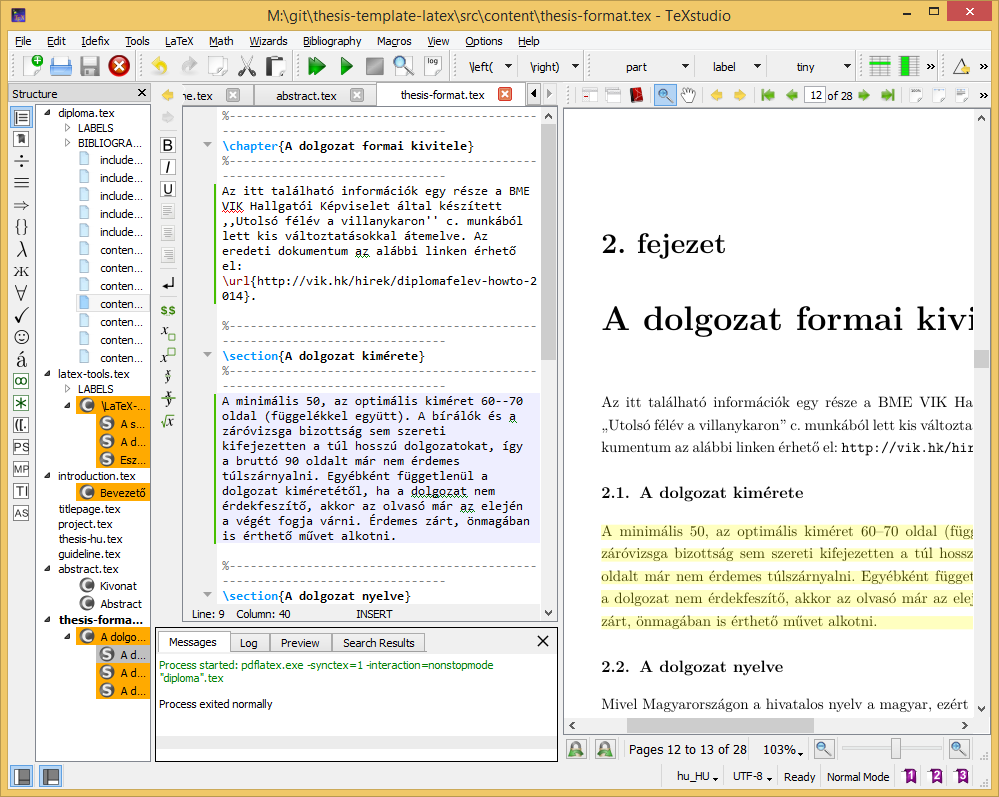
\includegraphics[width=150mm, keepaspectratio]{figures/TeXstudio.png}
\caption{A TeXstudio \LaTeX-szerkesztő.} 
\end{figure}

%----------------------------------------------------------------------------
\clearpage\section{Válasz az ,,Élet, a világmindenség, meg minden'' kérdésére}
%----------------------------------------------------------------------------
A Pitagorasz-tételből levezetve
\begin{align}
c^2=a^2+b^2=42.
\end{align}
A Faraday-indukciós törvényből levezetve
\begin{align}
\rot E=-\frac{dB}{dt}\hspace{1cm}\longrightarrow \hspace{1cm}
U_i=\oint\limits_\mathbf{L}{\mathbf{E}\mathbf{dl}}=-\frac{d}{dt}\int\limits_A{\mathbf{B}\mathbf{da}}=42.
\end{align}


%\label{page:last}
\end{document}
